\chapter{\texorpdfstring{Search for \Htohhtobbtautau}{Search for H -> hh -> bbtautau}}
\label{sec:hhh}

In this chapter the search for a heavy Higgs boson decaying to a pair of 125 GeV Higgs bosons, with one of these Higgs bosons decaying to 
a pair of b-jets and the other decaying to a pair of \Ptau leptons is discussed. This \Pgt-pair final states studied in this analysis
are the \etau, \mutau and \tautau channels. The results of this search are model-independent
upper limits on heavy Higgs production cross--section times branching ratio into h(125)h(125)$\rightarrow b\bar{b} \tau\tau$, which use
combine all three channels. The \etau and \mutau channels will be described in this chapter, the \tautau channel will not
be covered. In addition  the results are interpreted in the context of the MSSM and a type-II Two Higgs Doublet Model (2HDM), 
these interpretations are made in combination with the results of a search for \AtoZhtolltautau. 
This search will be summarised in this chapter, but will not constitute the main focus.
Both searches, and their interpretation, are detailed in reference \cite{CMS-HIG-14-034}.

The discovery of the 125 GeV Higgs boson by the ATLAS and CMS collaborations in 2012 \cite{HDiscoveryAtlas,HDiscoveryCMS} has opened up
new possibilities for probing the Higgs sector beyond the Standard Model. In some MSSM scenarios, and some more
generic type-II 2HDM's, a heavy neutral Higgs boson H can decay to a pair of 125 GeV Higgs bosons for low values
of \tanb, probing a region of phase space not yet excluded by stringent existing limits. In regions where
the decay \Htohh is enhanced, the \AtoZh decay also has a large branching ratio, indicating the usefulness
of both channels for probing the low-\tanb region. The $b\bar{b}$\tautau final state is chosen for the combination
of the large $h(125) \rightarrow b\bar{b}$ branching ratio and the cleaner \htotautau final state.

\section{Datasets and Monte Carlo samples}
\label{sec:hhh_datasets}
The dataset used for this analysis corresponds to the full dataset collected by the CMS experiment during the 2012 $p-p$ 
running period of the LHC. 
Signal and background events were generated using several different MC event generators. The \texttt{MadGraph}
\cite{madgraph} matrix element generator was used to generate samples of \Wjets, \Zellell, \ttbar and \ZZ ,\WZ and \WW
events. In addition to samples with a mixture of jet multiplicities ('inclusive' samples), samples binned in jet multiplicity
were used for the \Wjets and \Zellell backgrounds. This increases the number of background events
in signal regions with multiple jets. The samples binned in jet multiplicity are combined with the
inclusive samples such that the fraction of events with each jet multiplicity is preserved.

Single top samples were produced with the \texttt{POWHEG} \cite{powheg1,powheg2} generator. Samples of $gg\rightarrow$\Htohhtobbtautau
were generated in steps of 10 GeV between \mH $= 260 - 350$~GeV using \texttt{PYTHIA 6} \cite{pythia64}. In all of the samples
\texttt{TAUOLA} \cite{tauola} is used to decay $\tau$s, and parton showering and hadronisation are modelled using \texttt{PYTHIA 6} \cite{pythia64}.
Minimum bias events generated using \texttt{PYTHIA 6} are added to all MC samples to model additional
interactions. 

To better model the \Ztautau background, an embedding technique is used. In this method, 
\Zmm events are selected in data and the muons are replaced by generator-level taus. \texttt{TAUOLA} is used
to decay the taus and tau polarisation effectes are modelled using \texttt{TauSpinner} \cite{TauSpinner}. The detector
response to the tau decay products is modelled using the \texttt{GEANT4}-based \cite{Geant4} detector simulation, and 
tracks in the inner tracking system, hits in the muon systems and energy deposits in the calorimeters
due to the simulated taus are combined with the remains of the \Zmm event after the detector signals
of the two muons originiating from the \PZ have been removed. This technique is also applied to 
a \ttbar background samples to estimate the \ttbar contamination in the embedded sample. This contribution
needs to be subtracted from the \Ztautau background estimated using the embedded \Zmm sample to
avoid double counting with the \ttbar monte carlo.


\section{Event selection and categorisation}
\label{sec:hhh_selection}
A more detailed description of the physics objects used for this analysis is given in chapter FIXME:write object reco section, 
in this section only an overview of the event selection is presented.

\subsection{\texorpdfstring{Event selection in the \mutau channel}{Event selection in the mu-tau channel}}
\label{sec:hhh_selection_mutau}
Events in the \mutau channel are first selected by requiring a muon and a 
hadronic tau. The first step of this selection is a trigger which requires only a muon
at L1. At the level of the HLT a hadronic tau is also required. This is reconstructed
with a simpler version of the PF algorithm, and loose isolation requirements are 
applied. In addition, loose ID and isolation requirements are applied to the muon at 
this stage. 

In the offline event selection, an oppositely charged \mutau pair is required, 
separated by $\Delta R > 0.5$.
The muon is required to have a \pT of at 
least 20 GeV and $|\eta| < 2.1$, and should be compatible with originating from the 
primary vertex. This means the impact parameters $d_{xy}$ and $d_{z}$ must be smaller
than 0.045 and 0.2 cm respectively. Tight muon identification
criteria and tight isolation requirements $I_{\text{rel}}^{\mu} < 0.1$, as described 
in section OBJECTS, are applied. The hadronic tau must have a \pT of at least
20 GeV, $|\eta| < 2.3$, and must have $d_{z} < 0.2$ cm. It is required to pass 
the decay mode finding identification
from the HPS algorithm, as described in section OBJECTS. Additionally
the raw combined isolation, described in the same section, is required to be
at most 1.5 GeV. To reject $\Pe/\Pgm \rightarrow \Pgt_{h}$ fakes, and to
reduce the contribution of \Zmm background events, the hadronic tau is 
also required to pass the tight working point of the anti-$\Pgm$ discriminator
and the loose working point of the cut--based anti-$\Pe$ discriminator, both
described in section OBJECTS.

After this selection there is still a chance more than one possible 
\mutau pair exists
in the event. If this is the case, the combination with largest 
\pT$^{\Pgm}$ + \pT$^{\Pgt_{h}}$ is chosen. In order to reduce \Zmm 
backgrounds further, for cases where the reconstructed hadronic tau originates
from a misidentified jet, the event is rejected if an opposite--charge pair 
of lower \pT (at least 15 GeV) muons, passing looser ID and isolation requirements
than the signal muon, can be formed. Additional vetos, requiring exactly one muon and 
exactly zero electrons to pass \pT $>10$ GeV and tight ID and isolation requirements, 
are applied to reduce the \WZ background. 

In addition to the requirements on the di--tau pair, at least 2 jets with \pT$ >20$ GeV are 
required. No b--tagging requirements are applied at this stage, these will be discussed 
in more detail in section \ref{sec:hhh_selection_categories}.

Figure \ref{fig:Hhh_selection_kinematics_mt} shows some of the kinematic variables 
of di-\Pgt candidates in the \mutau channel
\begin{figure}[h!]
\begin{center}
 \subfloat[Muon \pT]{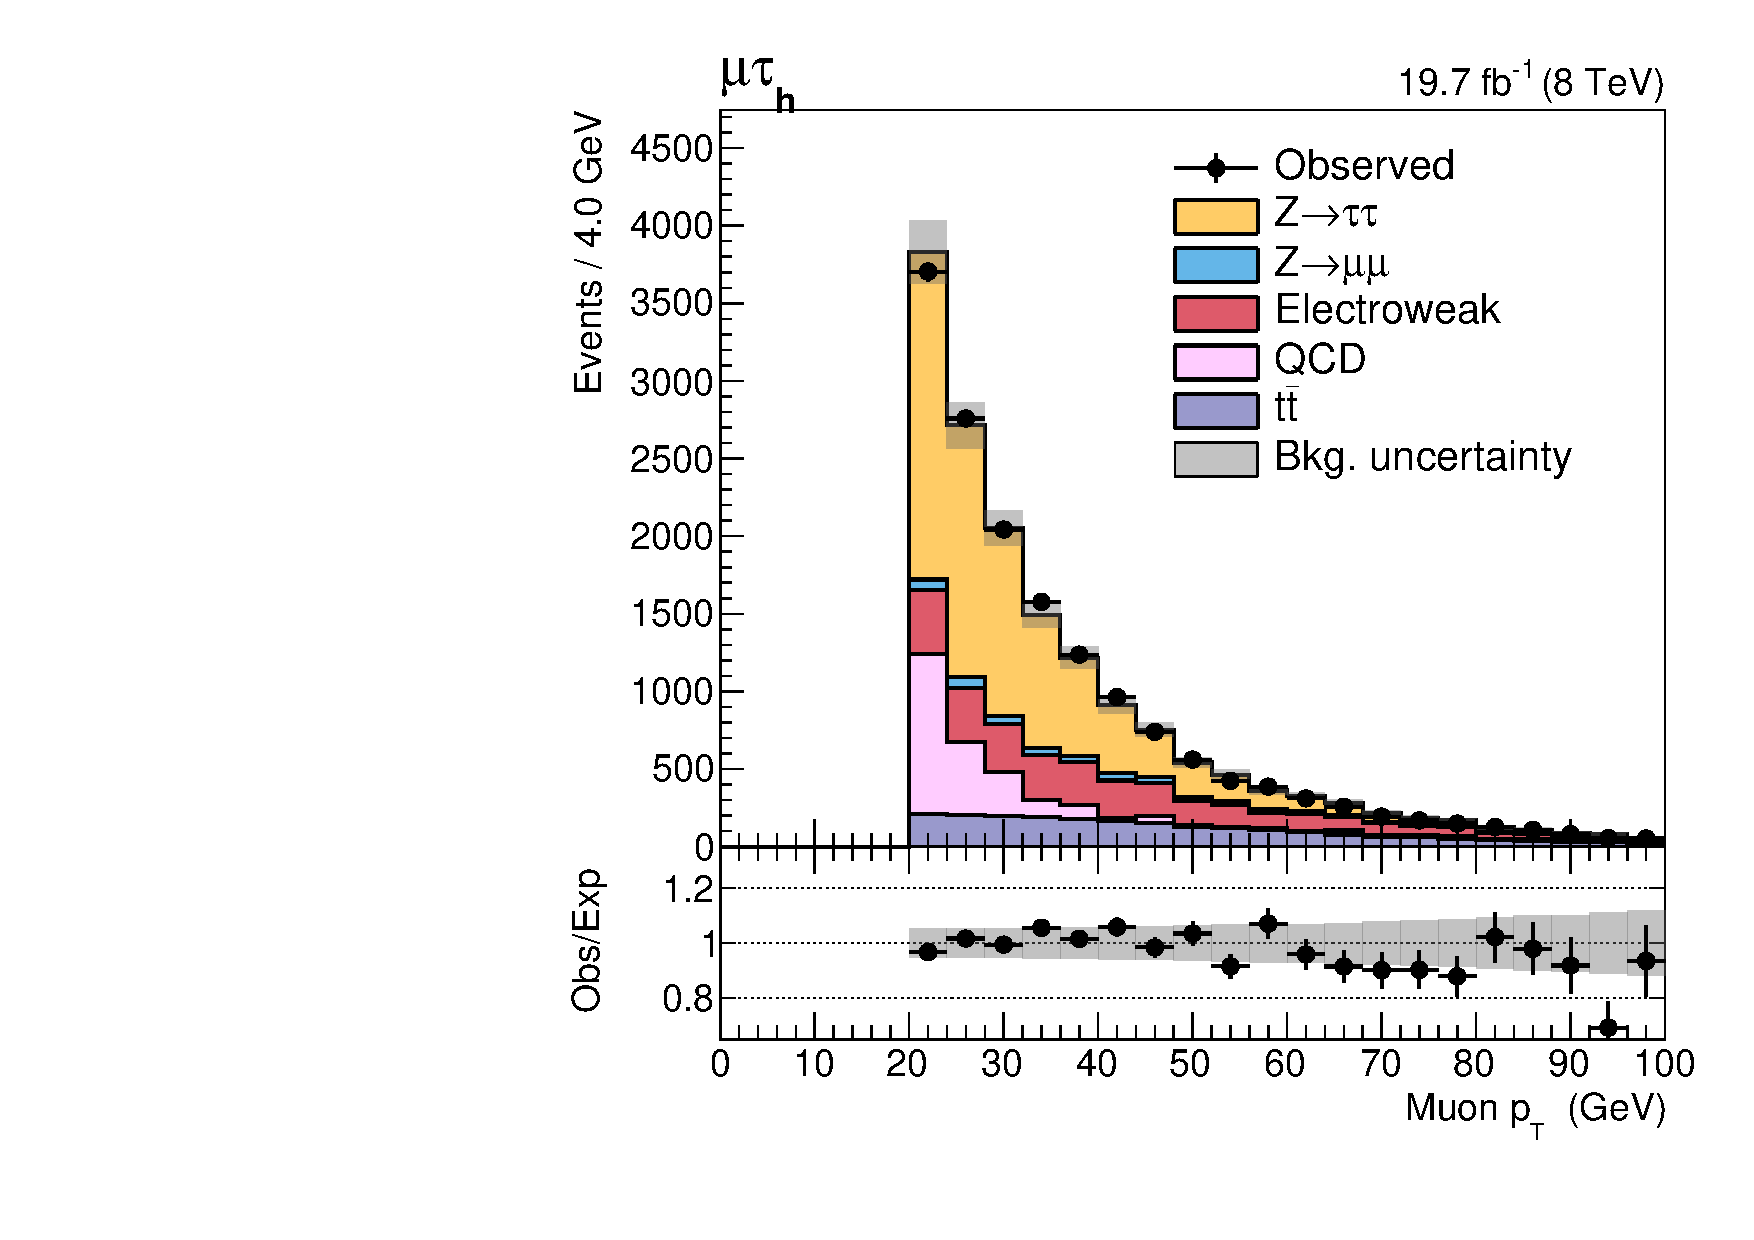
\includegraphics[width=0.5\textwidth]{Hhh/Plots/pt_1_2jetinclusive_mt_2012.pdf}}
  \subfloat[Hadronic \Pgt \pT ]{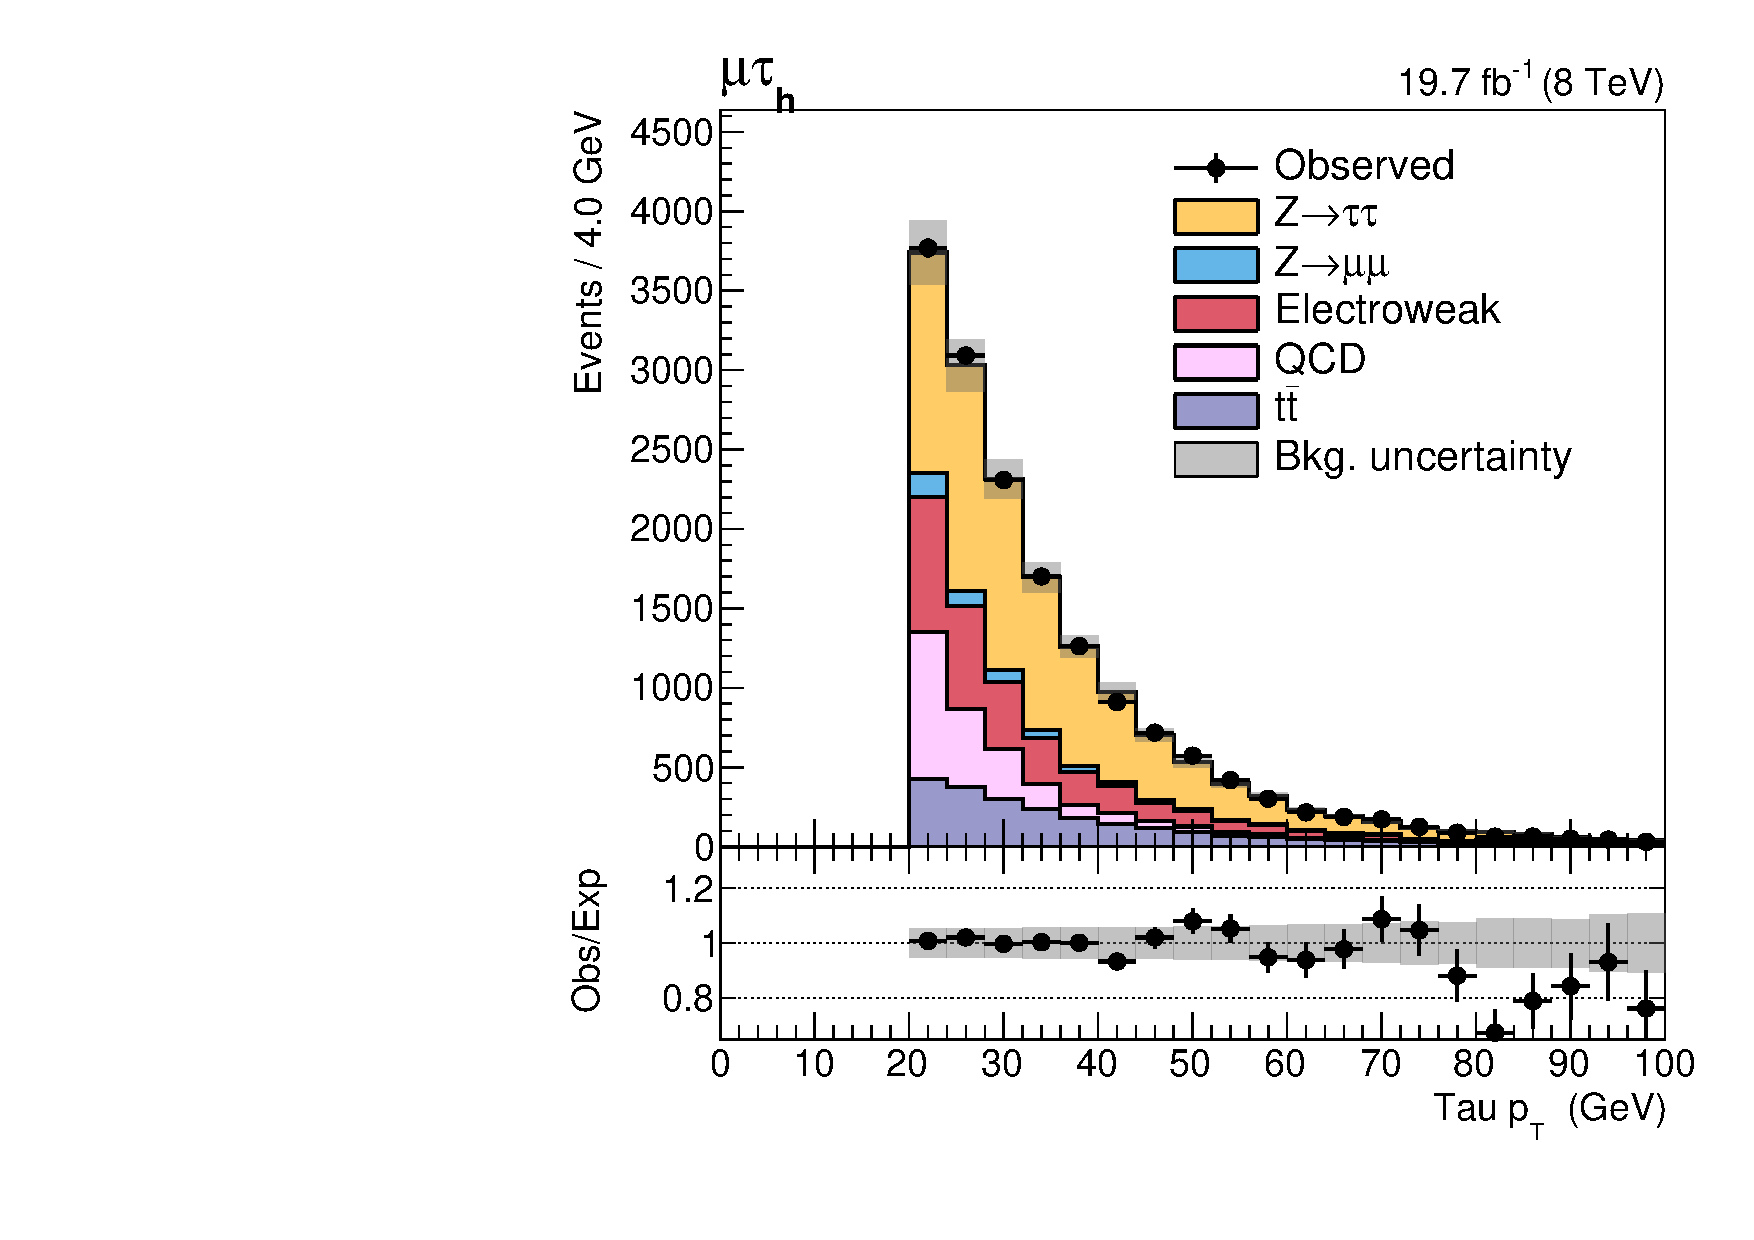
\includegraphics[width=0.5\textwidth]{Hhh/Plots/pt_2_2jetinclusive_mt_2012.pdf}}~\\
  \subfloat[Muon $\eta$]{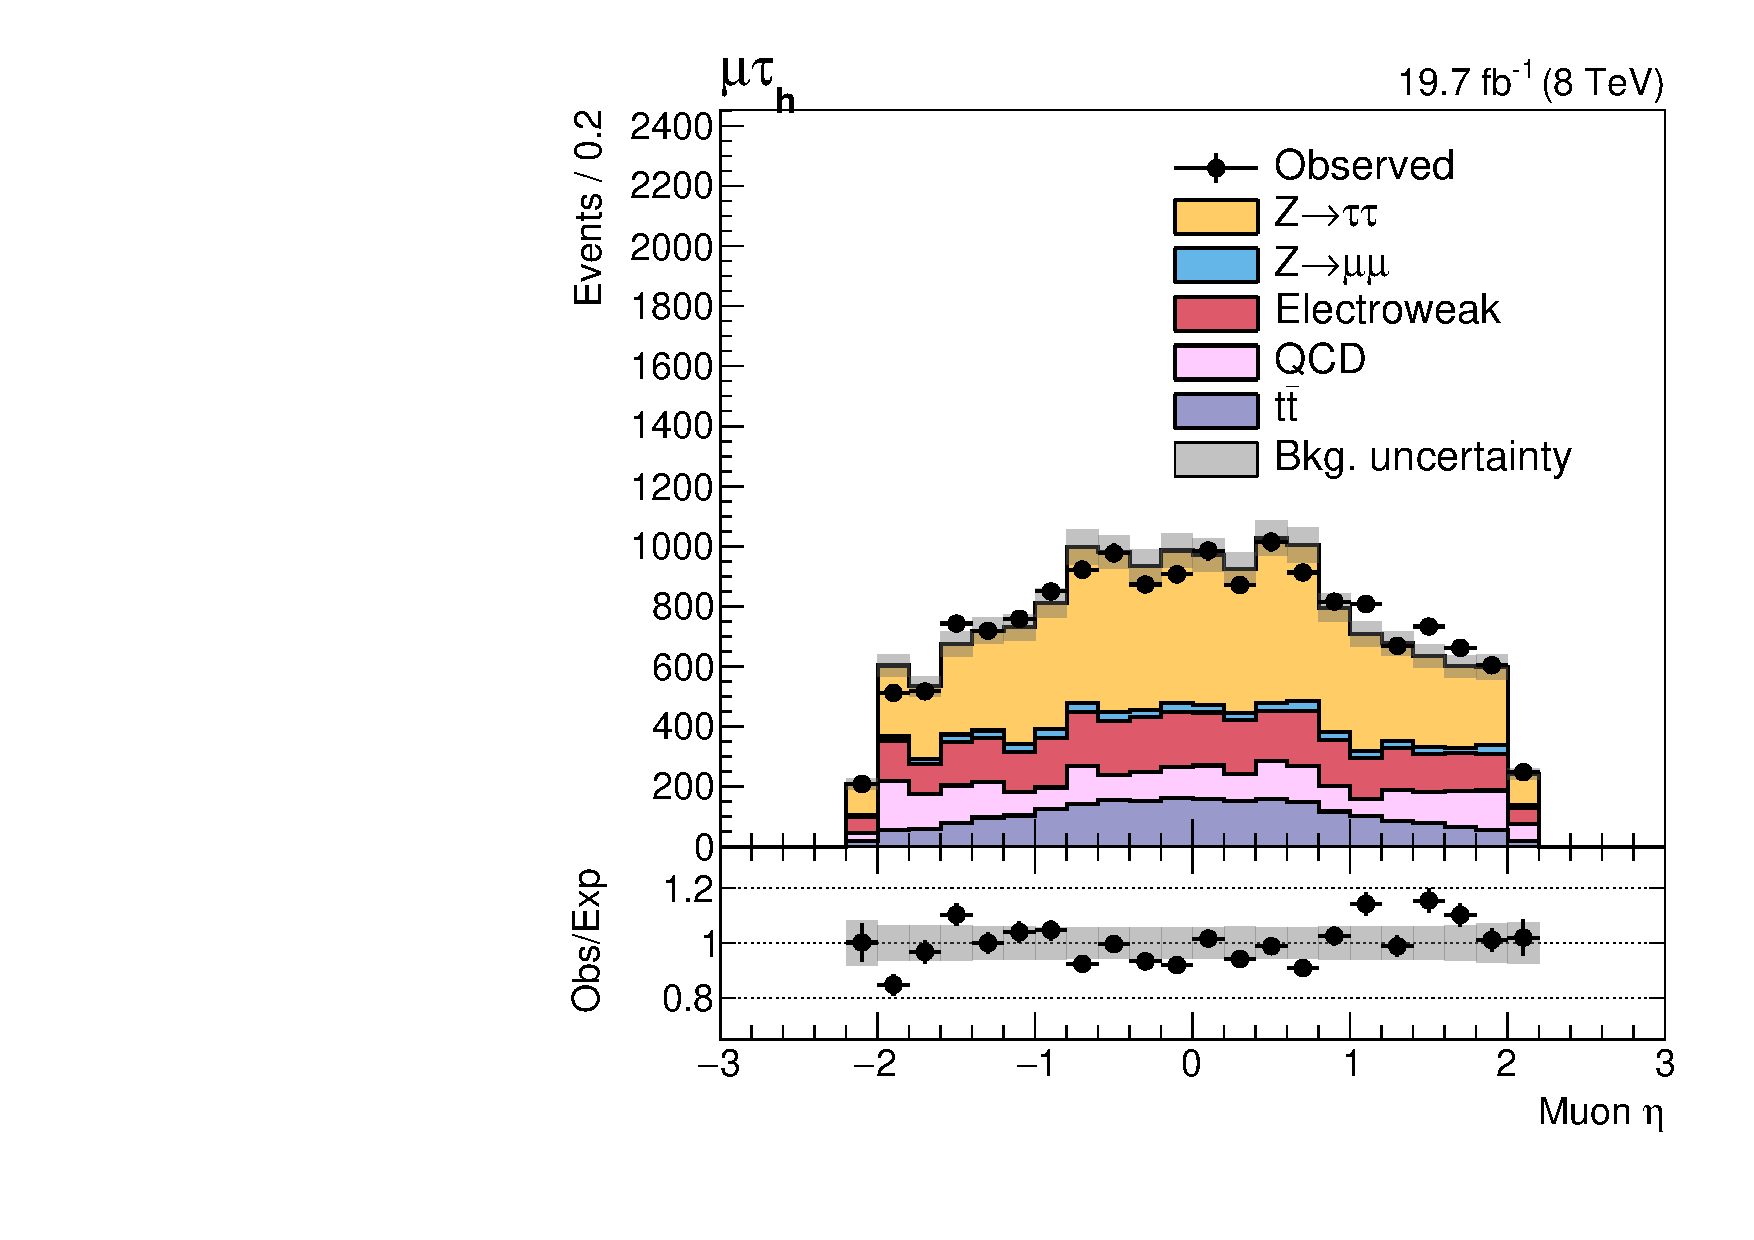
\includegraphics[width=0.5\textwidth]{Hhh/Plots/eta_1_2jetinclusive_mt_2012.pdf}}
  \subfloat[Hadronic \Pgt $\eta$ ]{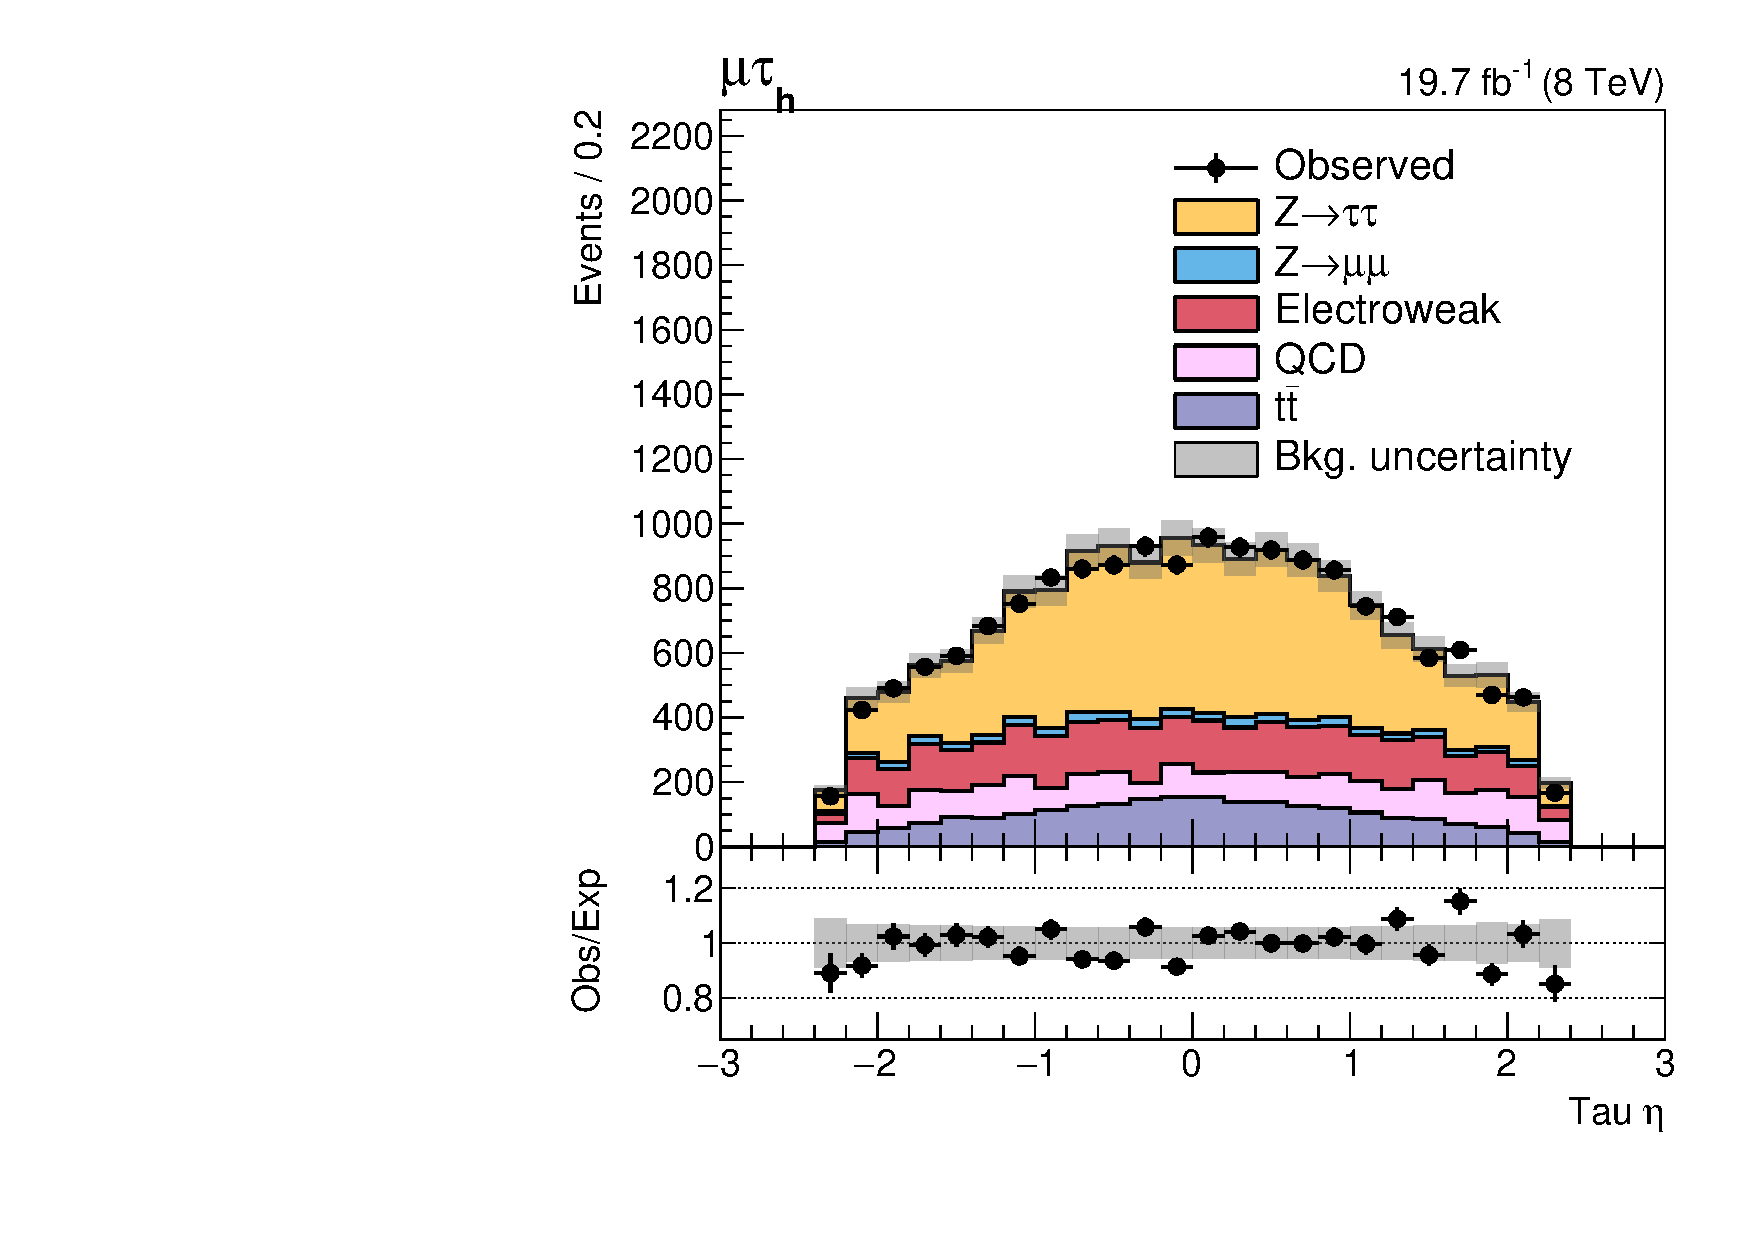
\includegraphics[width=0.5\textwidth]{Hhh/Plots/eta_2_2jetinclusive_mt_2012.pdf}}~\\

\end{center}
\caption{Plots of muon and hadronic \Pgt \pT and $\eta$ in the \mutau channel.}
\label{fig:Hhh_selection_kinematics_mt}
\end{figure}


\subsection{\texorpdfstring{Event selection in the \etau channel}{Event selection in the e-tau channel}}
\label{sec:hhh_selection_etau}
Events in the \etau channel are selected by requiring an electron and a hadronic tau.
As for the \mutau channel the first step of this selection is the trigger, which
requires an electron at L1, and both an electron and a hadronic tau at HLT. The hadronic
tau is reconstructed in a similar way to the \mutau channel, and loose ID and isolation requirements
are also applied to the electron.

Offline, an oppositely charged \etau pair is required, again separated by $\Delta R >0.5$. 
The electron should have a \pT of at least 24 GeV, $|\eta| < 2.1$, and should
satisfy $d_{xy} < 0.045$cm and $d_{z} < 0.2$ cm. The electron must pass the tight
working point of the electron MVA ID discriminator described in section OBJECTS, and the
relative isolation is required to be $I_{rel}^{\Pe} < 0.1$. The requirements placed on the
hadronic tau are similar to those required in the \mutau channel, apart from the anti-$\Pgm$ discriminator,
where the loose working point is required, and the anti--$\Pe$ discriminator, where the medium
working point of the MVA discriminator is required.

If there is more than one possible \etau pair, the pair with largest \pT$^{\Pe}$+\pT$^{\Pgt_{h}}$
is taken. Similar additional vetos as in the \mutau channel are applied.
the event is rejected if an opposite--charge pair of \pT $> 15$ GeV electrons, passing looser ID and
isolation requirements than the signal electron requirements can be formed. To reduce the \WZ
background events that have more than one electron or at least one muon passing \pT $>10$ GeV and tight ID and isolation
requirements are rejected.

In addition to the requirements on the di--tau pair, at least 2 jets with \pT $>20$ GeV are 
required. 

Figure \ref{fig:Hhh_selection_kinematics_et} shows some of the kinematic variables 
of di-\Pgt candidates in the \etau channel
\begin{figure}[h!]
\begin{center}
 \subfloat[Electron \pT]{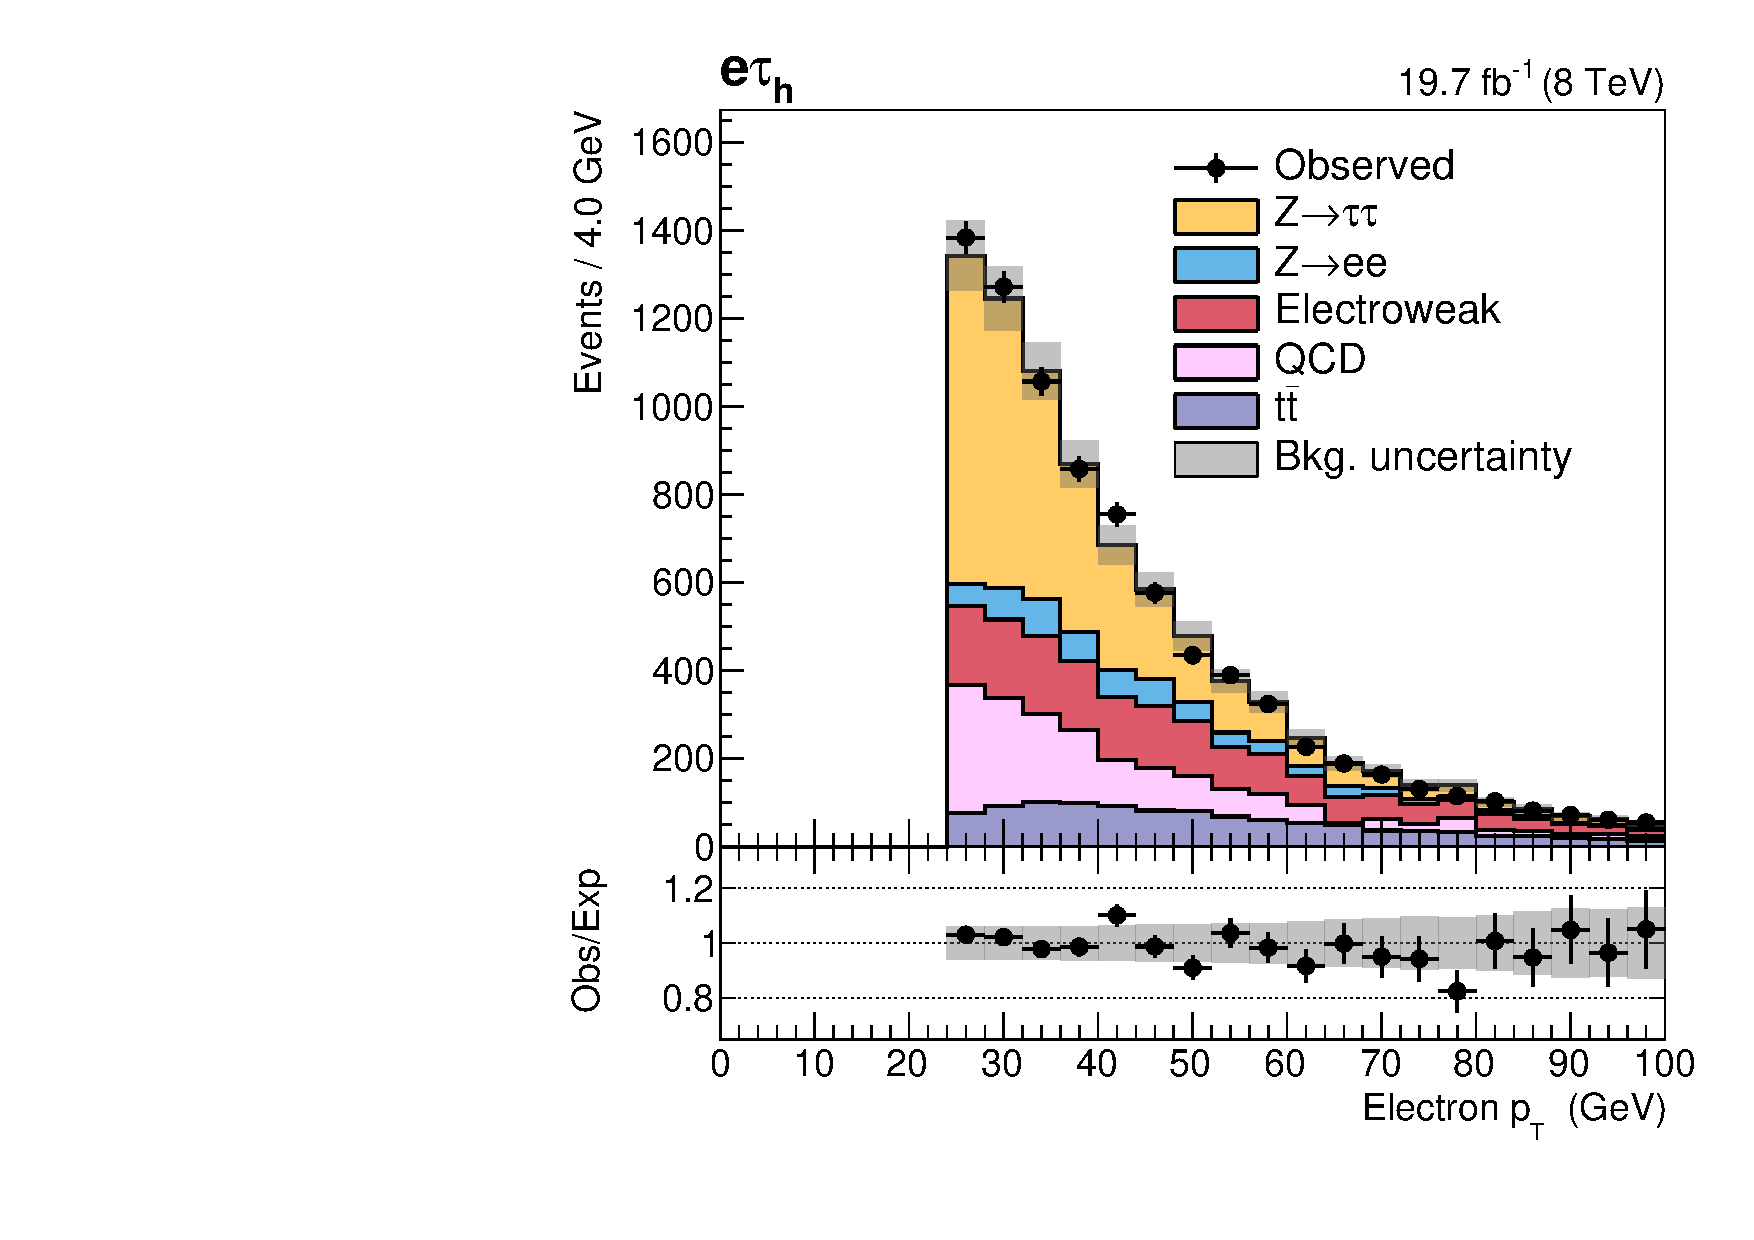
\includegraphics[width=0.5\textwidth]{Hhh/Plots/pt_1_2jetinclusive_et_2012.pdf}}
  \subfloat[Hadronic \Pgt \pT ]{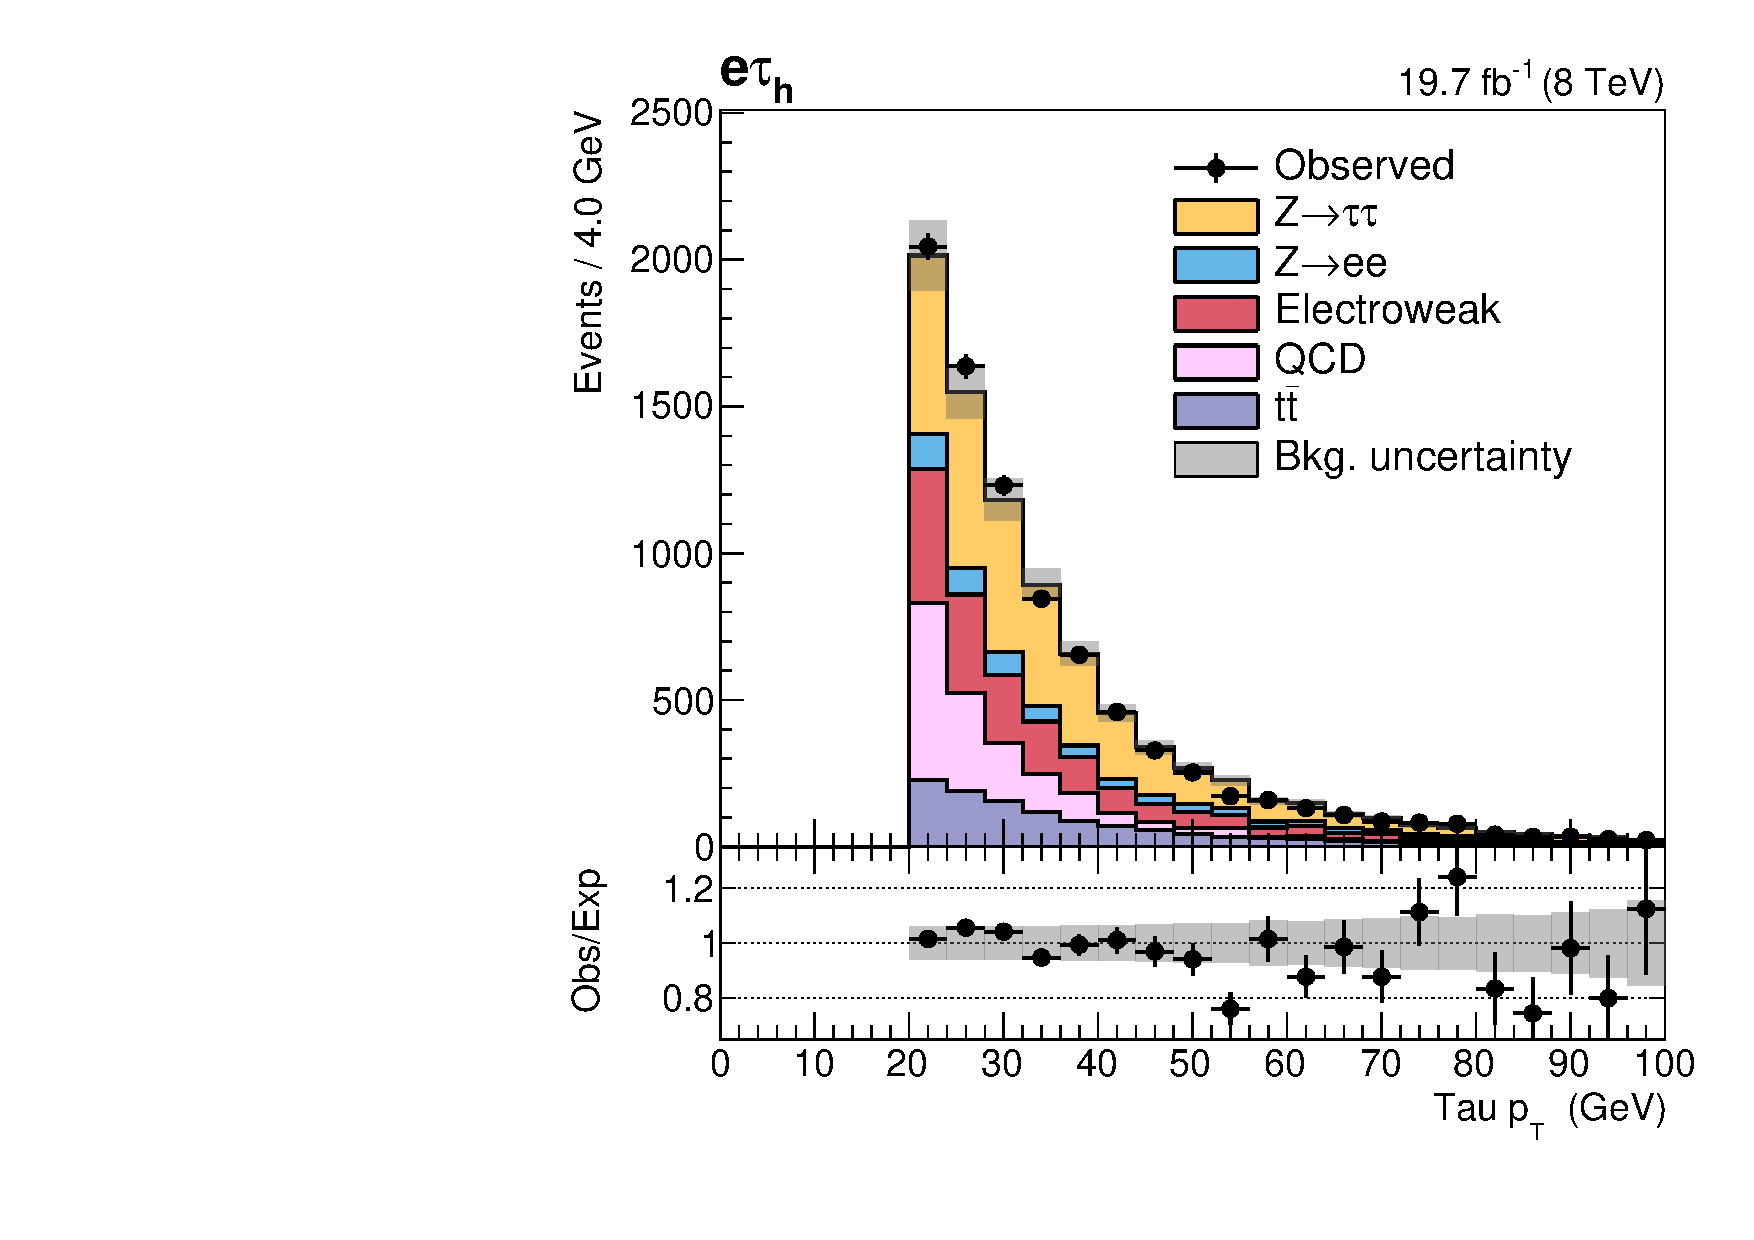
\includegraphics[width=0.5\textwidth]{Hhh/Plots/pt_2_2jetinclusive_et_2012.pdf}}~\\
  \subfloat[Electron $\eta$]{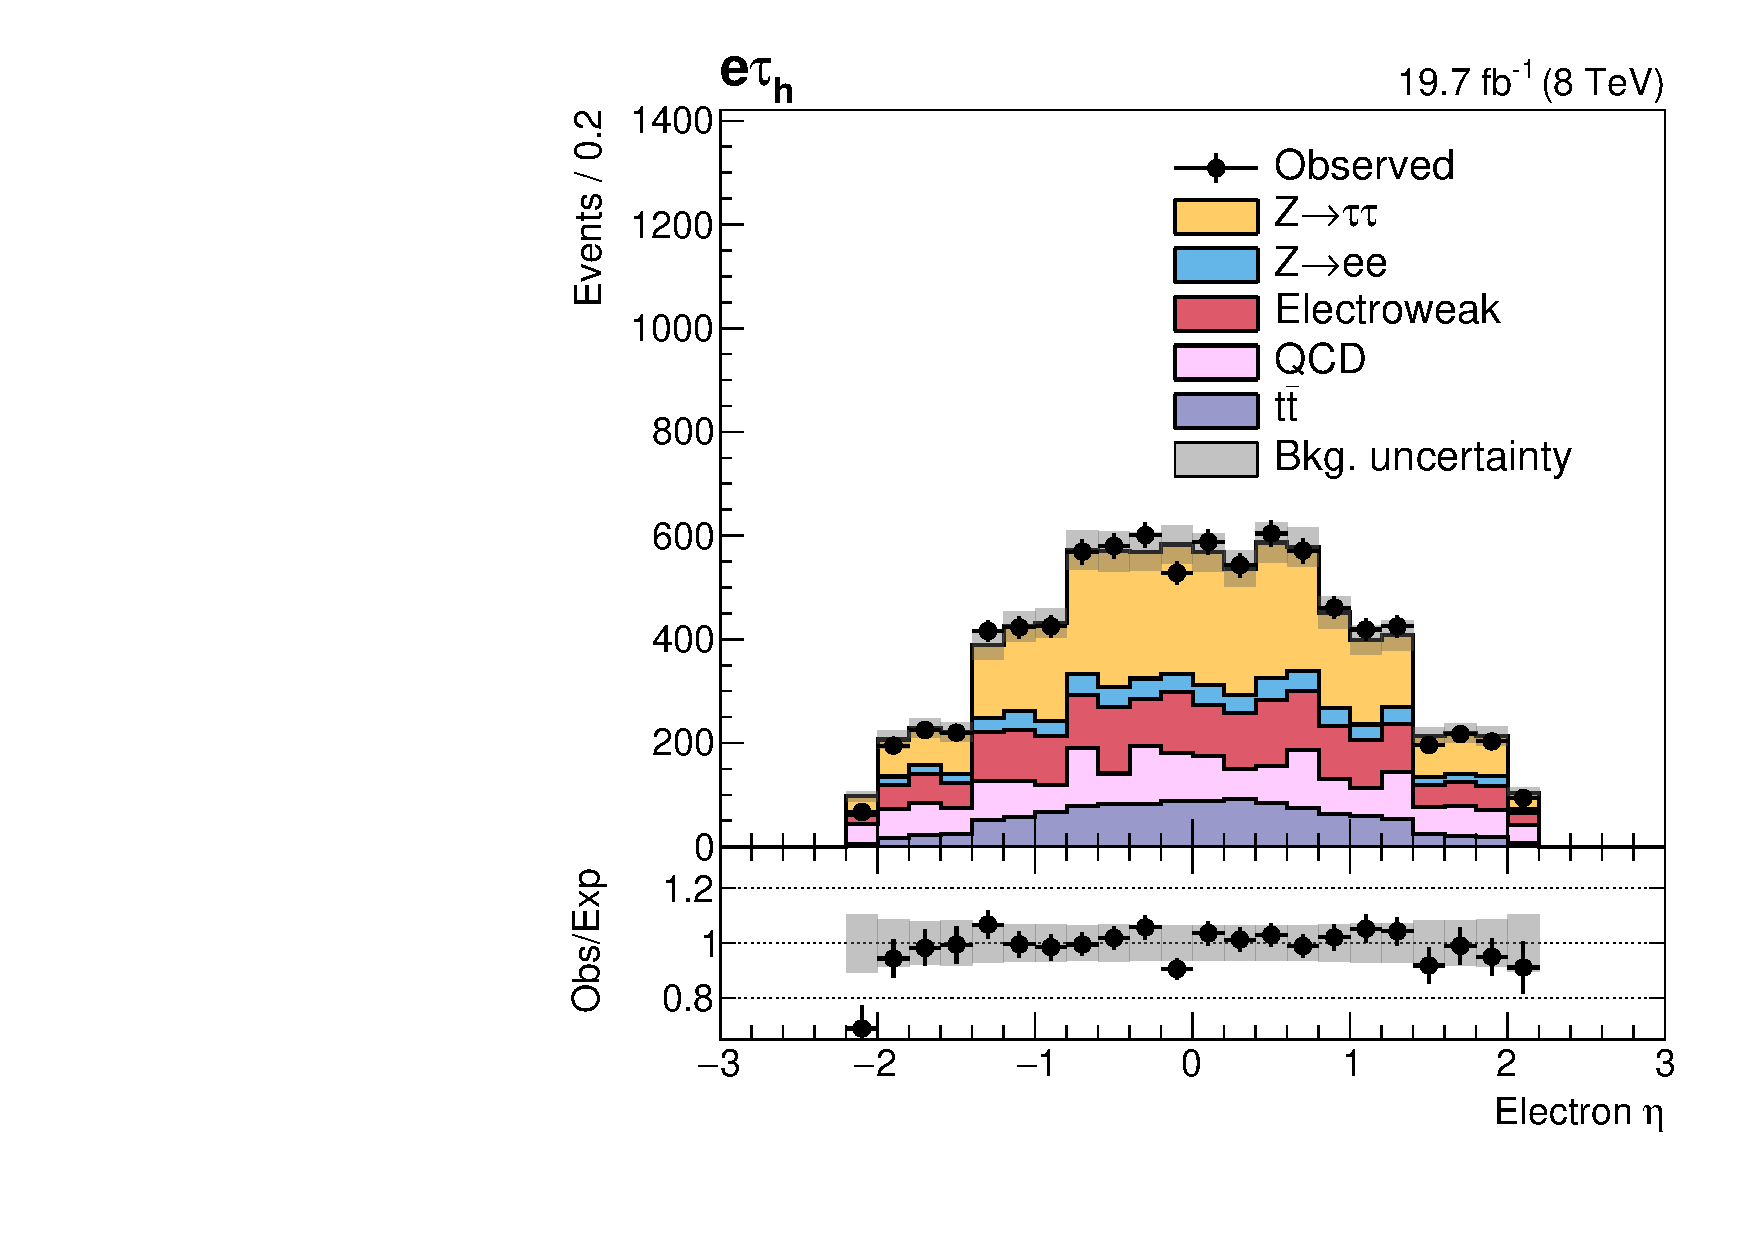
\includegraphics[width=0.5\textwidth]{Hhh/Plots/eta_1_2jetinclusive_et_2012.pdf}}
  \subfloat[Hadronic \Pgt $\eta$ ]{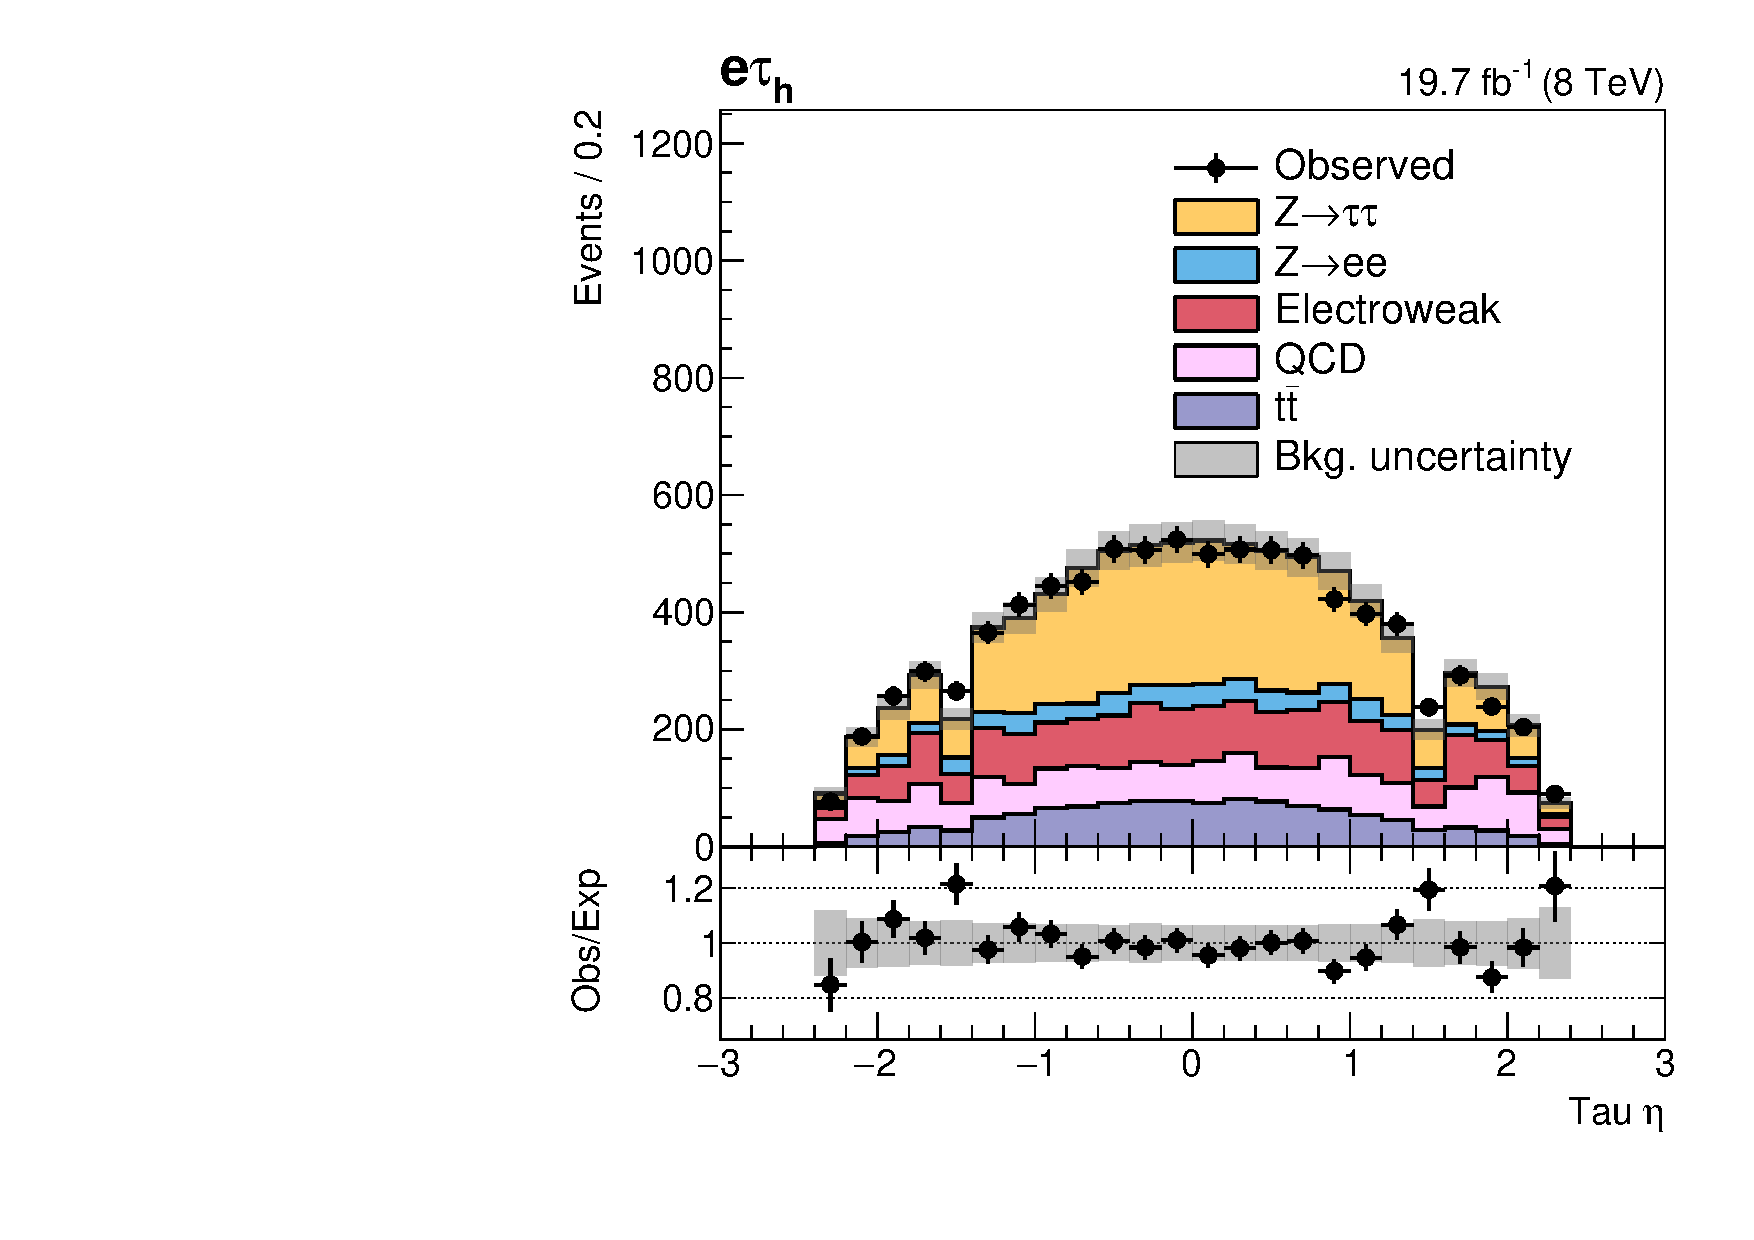
\includegraphics[width=0.5\textwidth]{Hhh/Plots/eta_2_2jetinclusive_et_2012.pdf}}~\\

\end{center}
\caption{Plots of electron and hadronic \Pgt \pT and $\eta$ in the \etau channel.}
\label{fig:Hhh_selection_kinematics_et}
\end{figure}


\subsection{Categorisation}
\label{sec:hhh_selection_categories}
ADD b-jet plots?
In both channels an selection on the transverse mass \mT between the electron/muon
and missing transverse energy, defined as in equation \ref{eqn:hhh_selection_mt}, is applied.

\begin{equation}\label{eqn:hhh_selection_mt}
m_{\text{T}} = \sqrt{2p_{\text{T}}E_{\text{T}}^{\text{miss}}(1-\cos{\Delta\phi})}
\end{equation}

In this eqation \pT is the transverse momentum of the electron or muon, and $\Delta\phi$ the angle
between the light lepton and the missing transverse energy. The \mT distributions for the \etau
and \mutau channels, using the selections as
described in sections \ref{sec:hhh_selection_mutau} and \ref{sec:hhh_selection_etau},
is shown in figure \ref{fig:Hhh_selection_mt}

\begin{figure}[h!]
\begin{center}
\subfloat[\mutau channel]{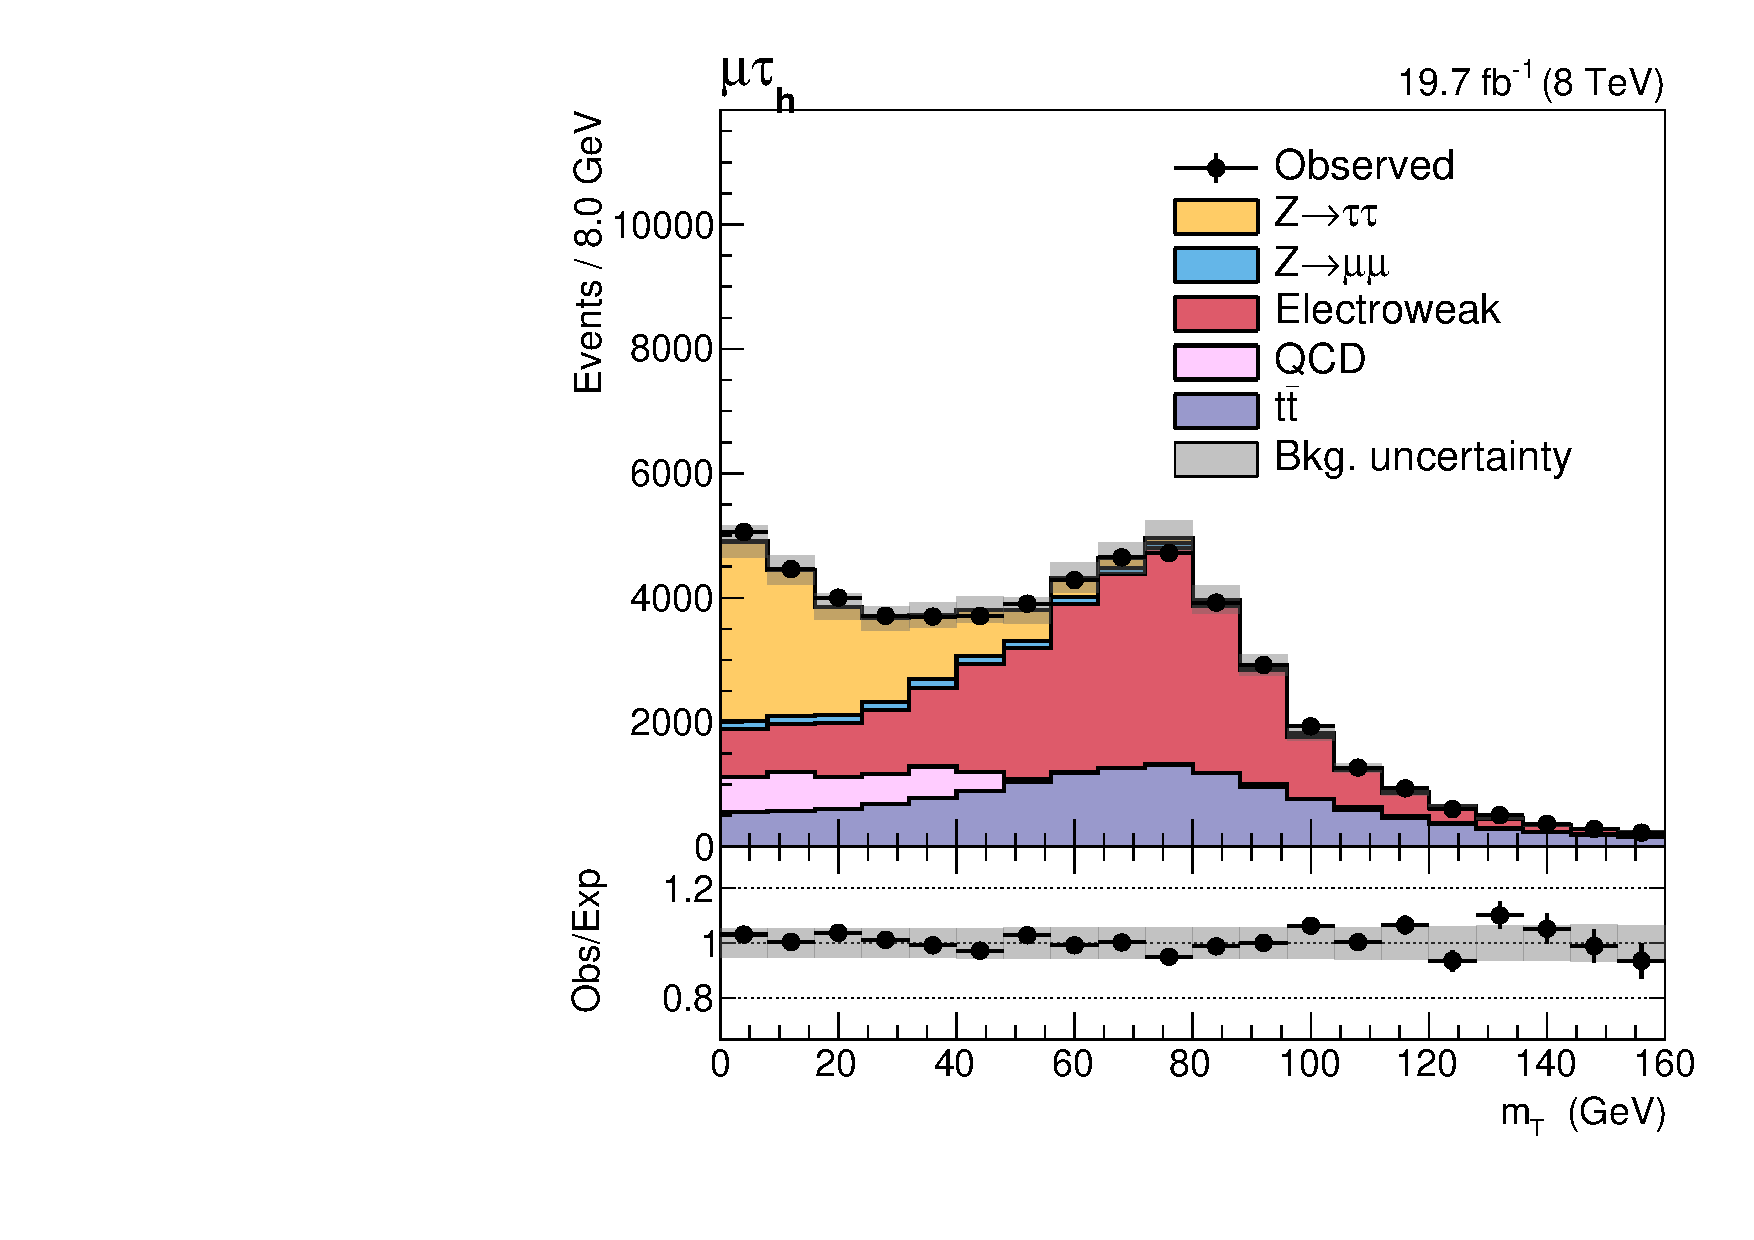
\includegraphics[width=0.5\textwidth]{Hhh/Plots/mt_1_2jetinclusive_mt_2012.pdf}}
\subfloat[\etau channel]{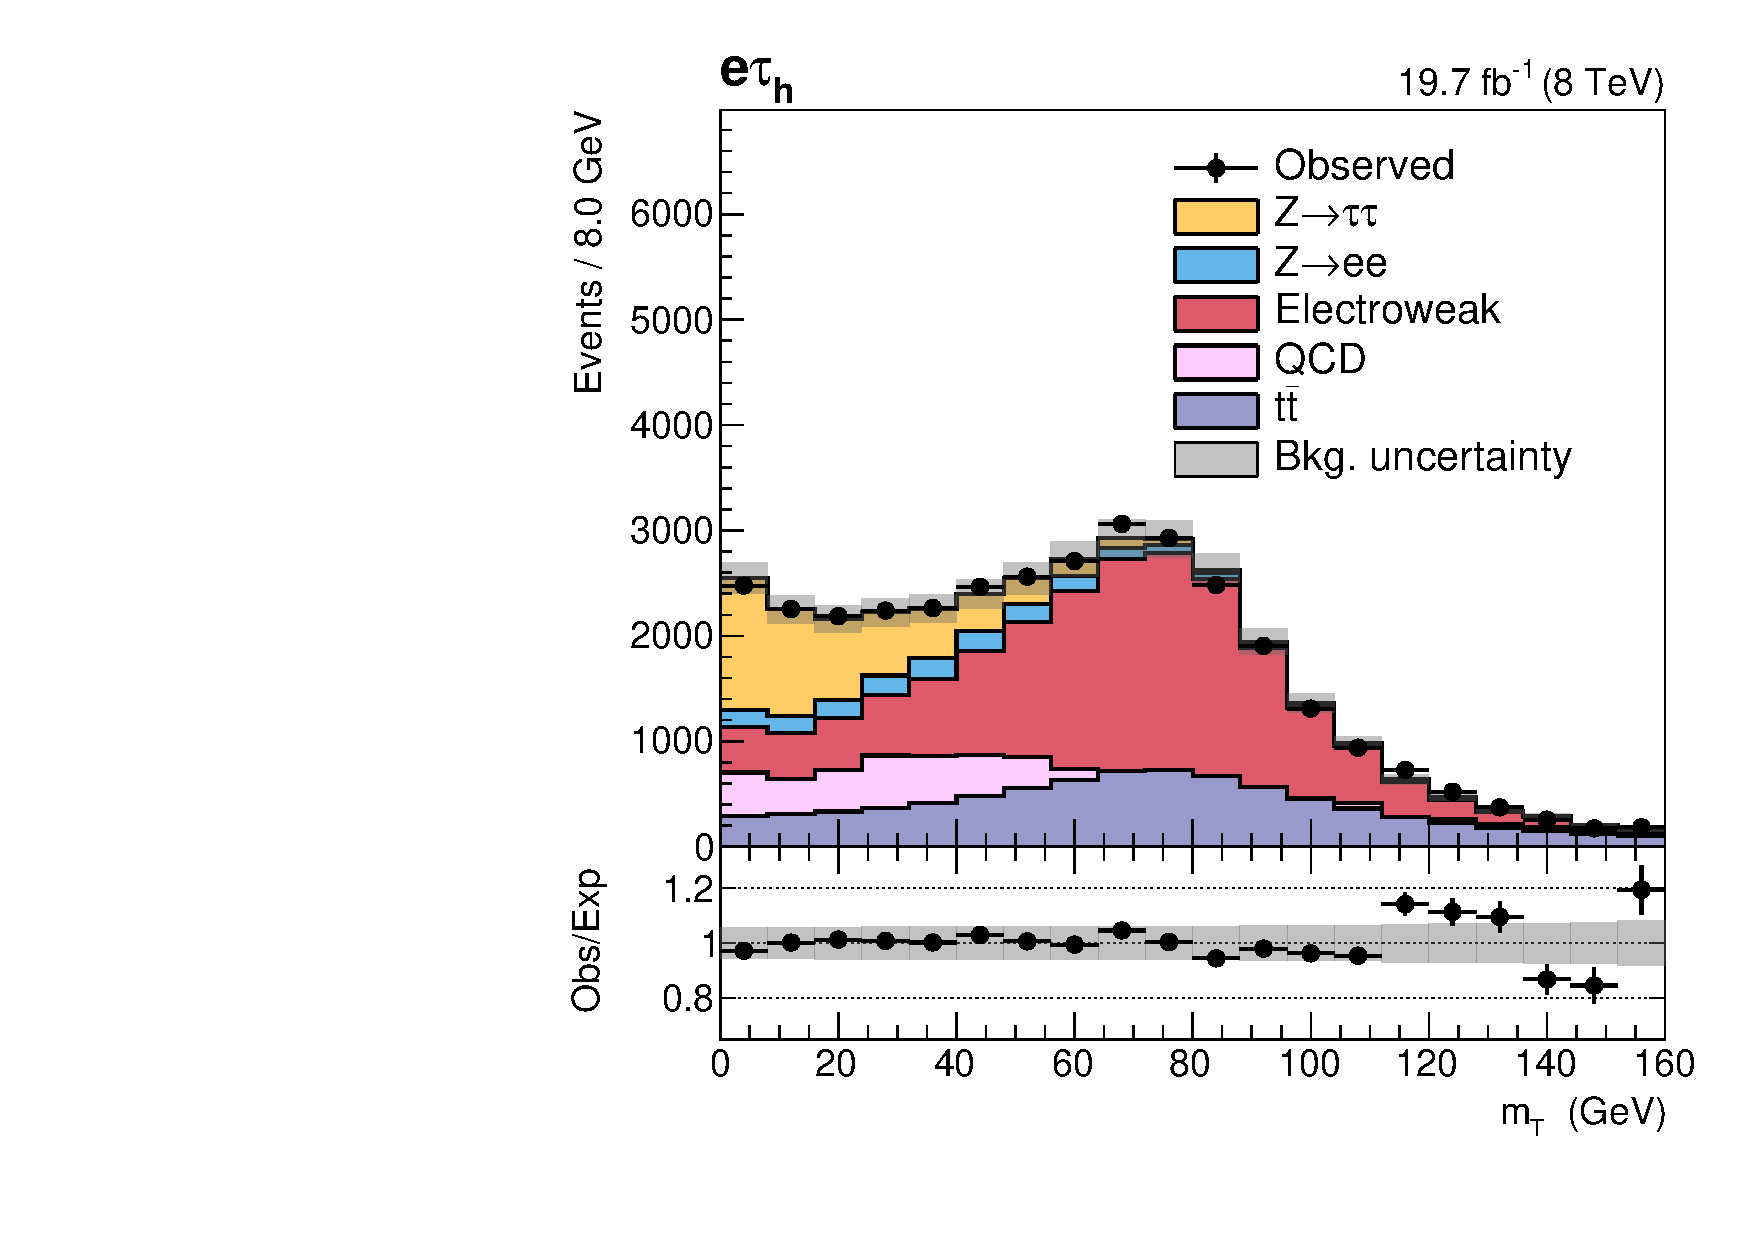
\includegraphics[width=0.5\textwidth]{Hhh/Plots/mt_1_2jetinclusive_et_2012.pdf}}
\end{center}
\caption{\mT distributions in the \mutau (left) and \etau (right) channels}
\label{fig:Hhh_selection_mt}
\end{figure}

In both channels this quantity is required to be smaller than 30 GeV. In events
where the missing energy and the light lepton are oriented back--to--back, \mT is
large, whereas it is closer to zero when the two are aligned. In $\PW\rightarrow\ell\nu$
events, as the W is very heavy, the lepton and neutrino are more likely to emitted back--to--back,
therefore \mT will be large. For \Ztautau and \htotautau events, in a $\tau\rightarrow\ell\nu\nu$ decay 
the neutrinos are more likely to travel in the same direction as the visible decay products of 
the tau, due to the smaller mass of the \Pgt compared with the \PW. Therefore requiring the
transverse mass to be less than 30 GeV reduces the \Wjets background. This effect
is also visible in figure \ref{fig:Hhh_selection_mt}, where the \Wjets and the much
smaller diboson and single-top backgrounds are drawn together as 'electroweak backgrounds'.
%In this analysis the presence of at least 2 jets increases the relative fraction of \ttbar 
%background events. Because the missing energy can now originate from multiple
%heavy objects (two tops) the missing transverse energy alignment is randomised. In some
%cases the lepton and missing transverse energy can be very much like the W decay
%topology, whereas in other cases \mT will be lower

After applying the \mT selection, events are divided into three categories to maximise
sensitivity to the signal: 2jet-0tag (at least 2 jets, exactly 0 of which are b-tagged), 2jet-1tag 
(at least 2 jets, exactly 1 of which is b-tagged), 2jet-2tag (at least 2 jets, at least 2 of which are b-tagged).
The 2jet-0tag category does not collect much of the signal and is dominated by 
backgrounds, the 2jet-2tag category is most sensitive to signal. 
In signal events, the di--tau pair and di--jet pair 
are the decay products of an 125 Gev Higgs boson, therefore their invariant
masses should be close to 125 GeV. To reduce background contributions
from events where the di--tau or di--jet mass is not compatible with
125 GeV, requirements are made on the di--jet invariant mass and the di--tau
invariant mass as reconstructed using the \texttt{SVFit} algorithm (ADD A SECTION ON THIS).
By requiring $70 < m_{jj} < 150 $GeV and $90 < m_{\Pgt\Pgt} < 150$ GeV a 
large number of background events can be rejected, while retaining
most of the signal. This is illustrated in figure \ref{fig:Hhh_selection_masscuts} for 
the 2jet-2tag category.

\begin{figure}[h!]
\begin{center}
\subfloat[$m_{\Pgt\Pgt}$ (\mutau channel)]{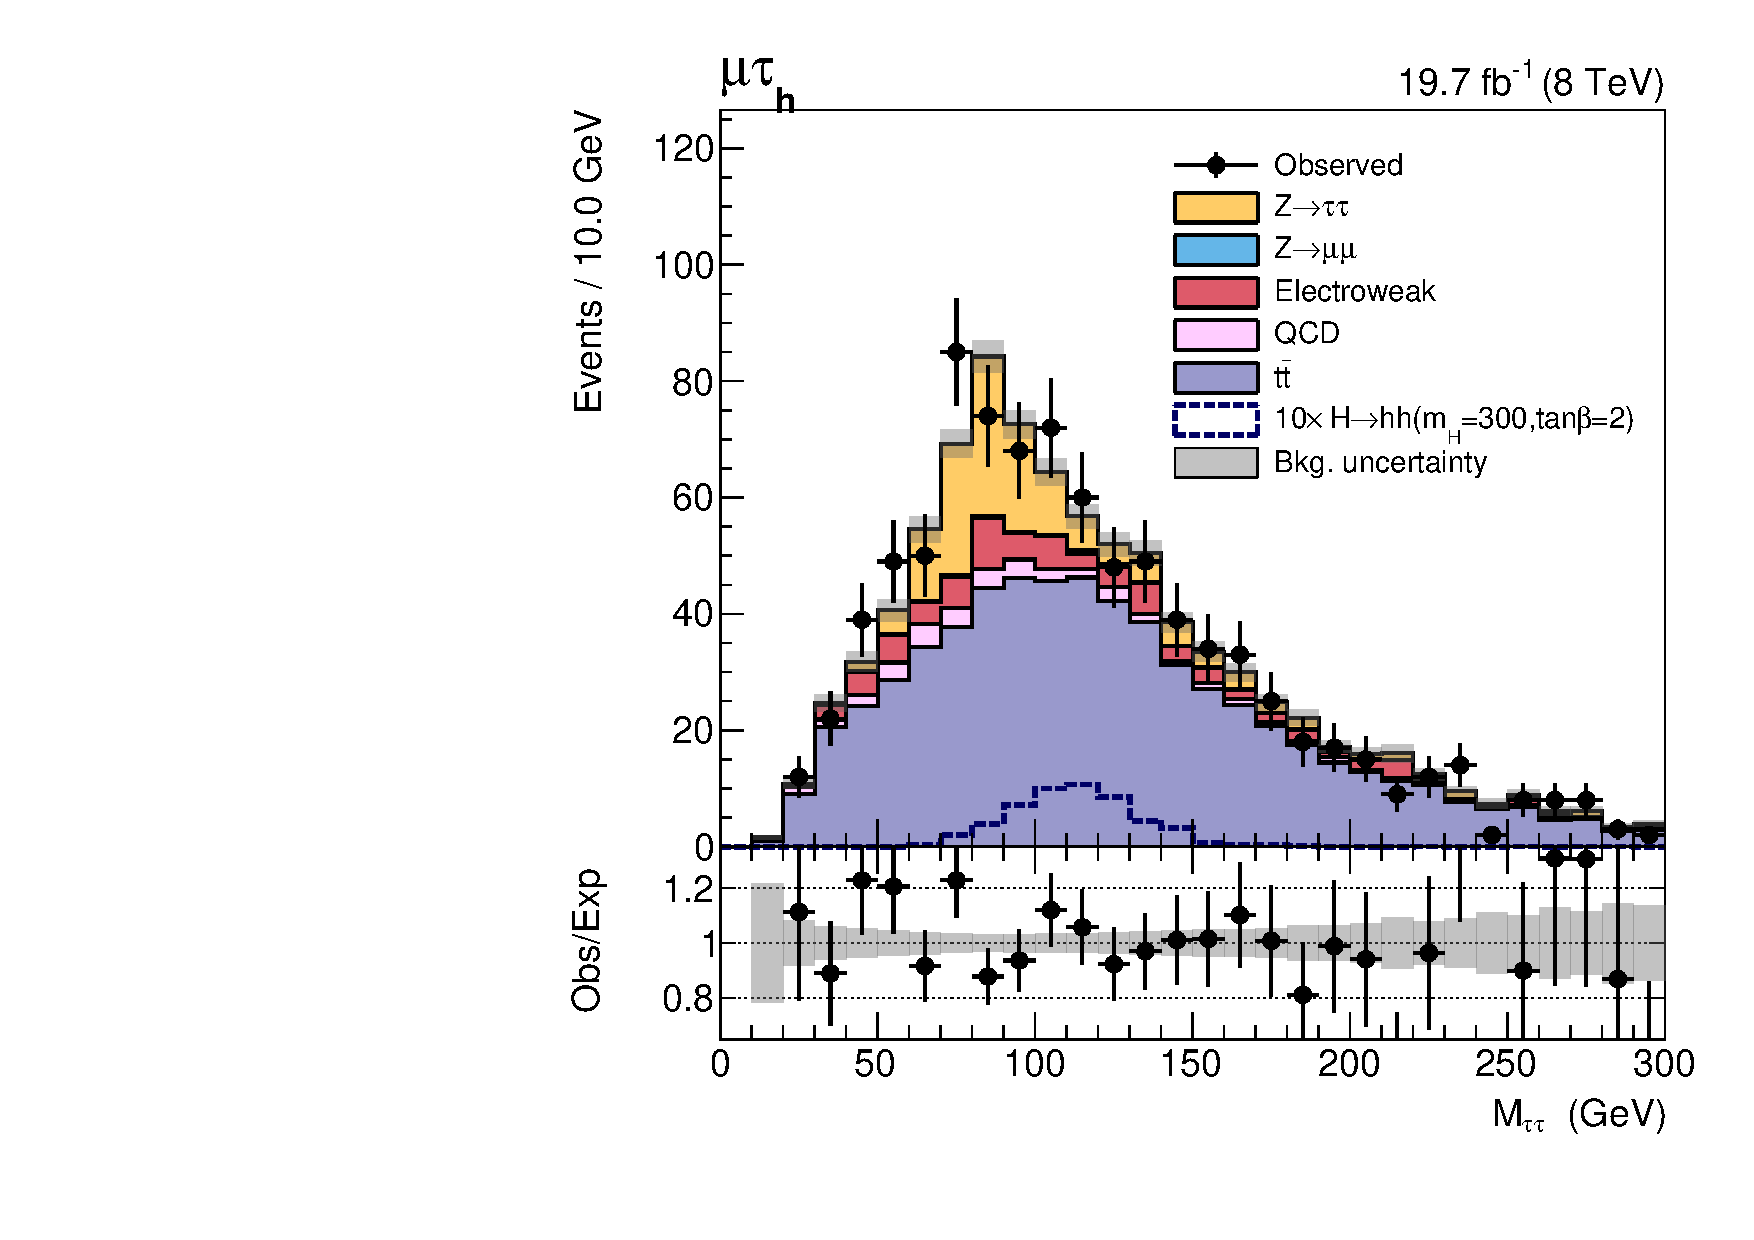
\includegraphics[width=0.5\textwidth]{Hhh/Plots/m_sv_2jet2tag_mt_2012.pdf}}
\subfloat[$m_{\Pgt\Pgt}$ (\etau channel)]{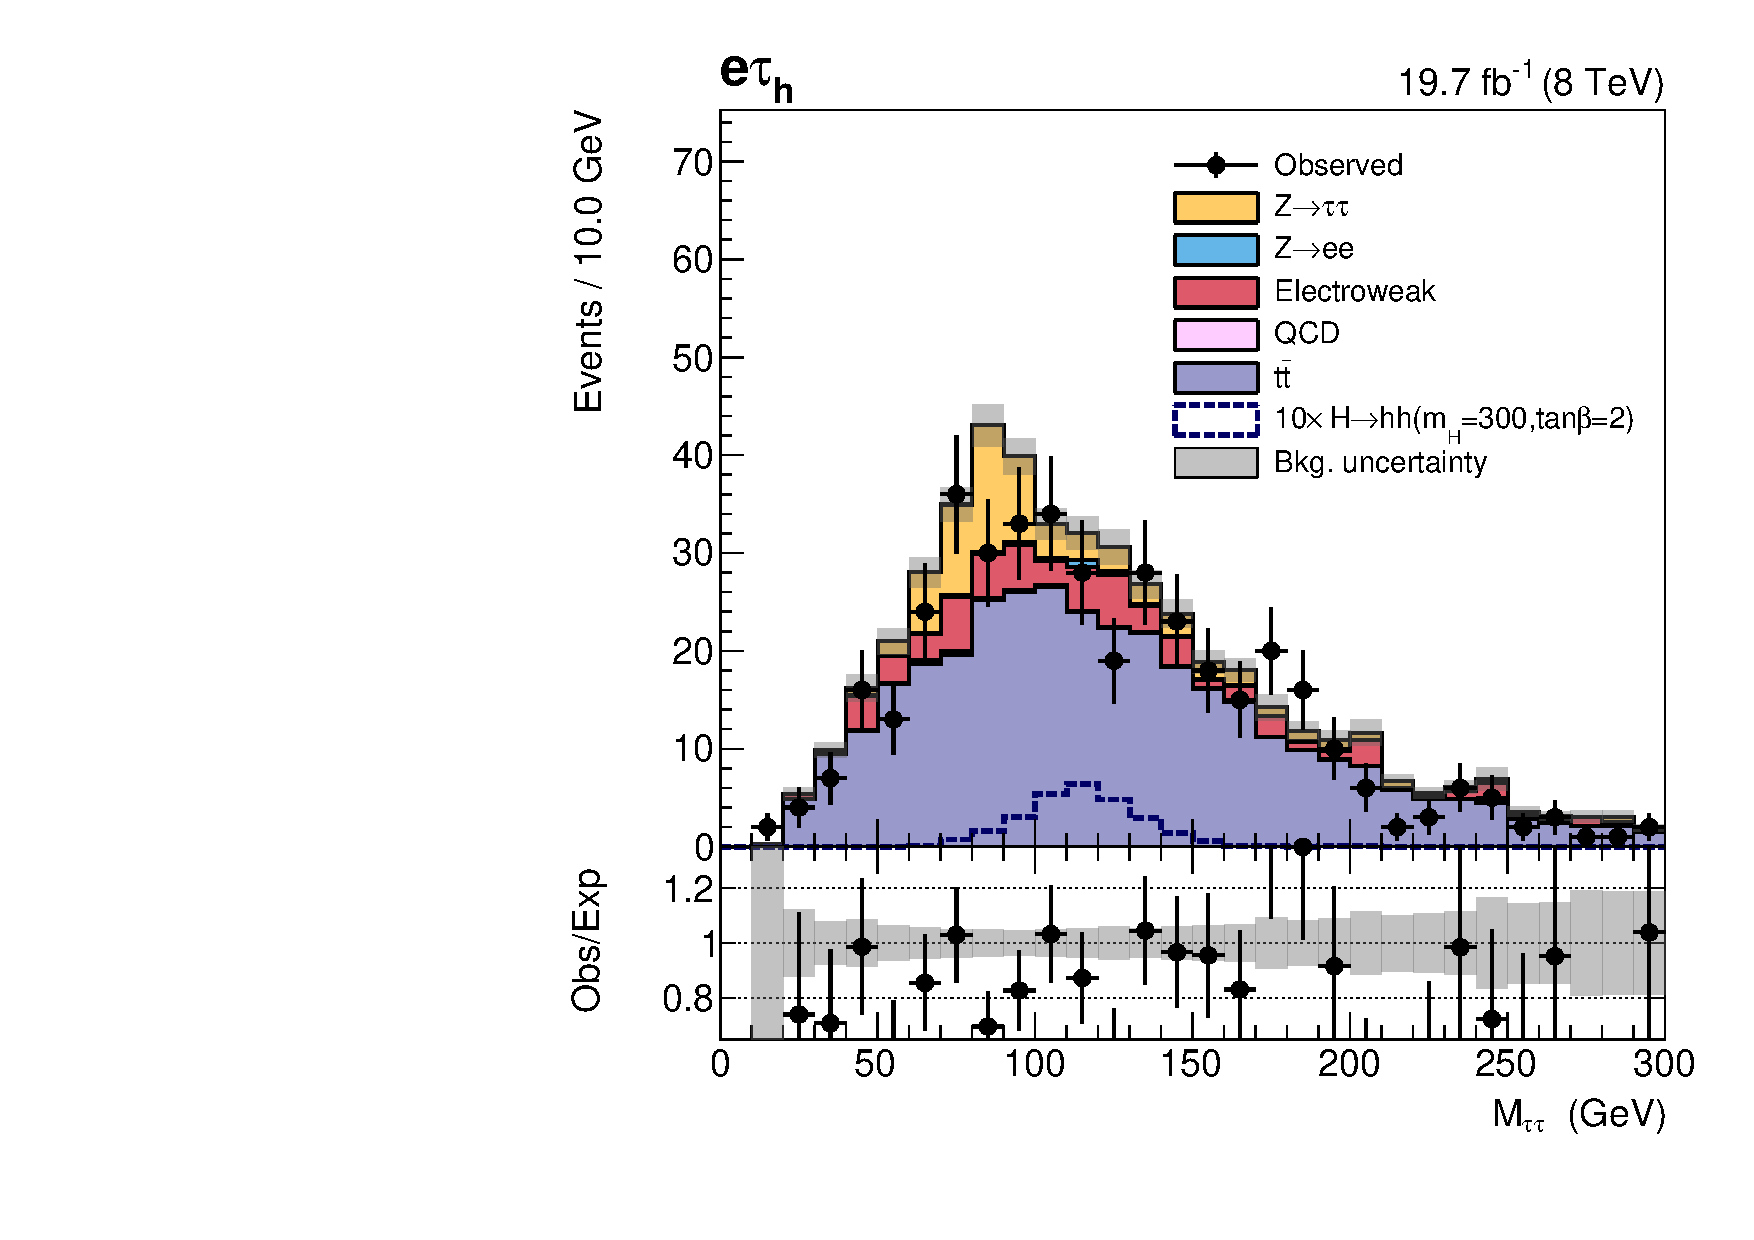
\includegraphics[width=0.5\textwidth]{Hhh/Plots/m_sv_2jet2tag_et_2012.pdf}}~\\
\subfloat[$m_{jj}$ (\mutau channel)]{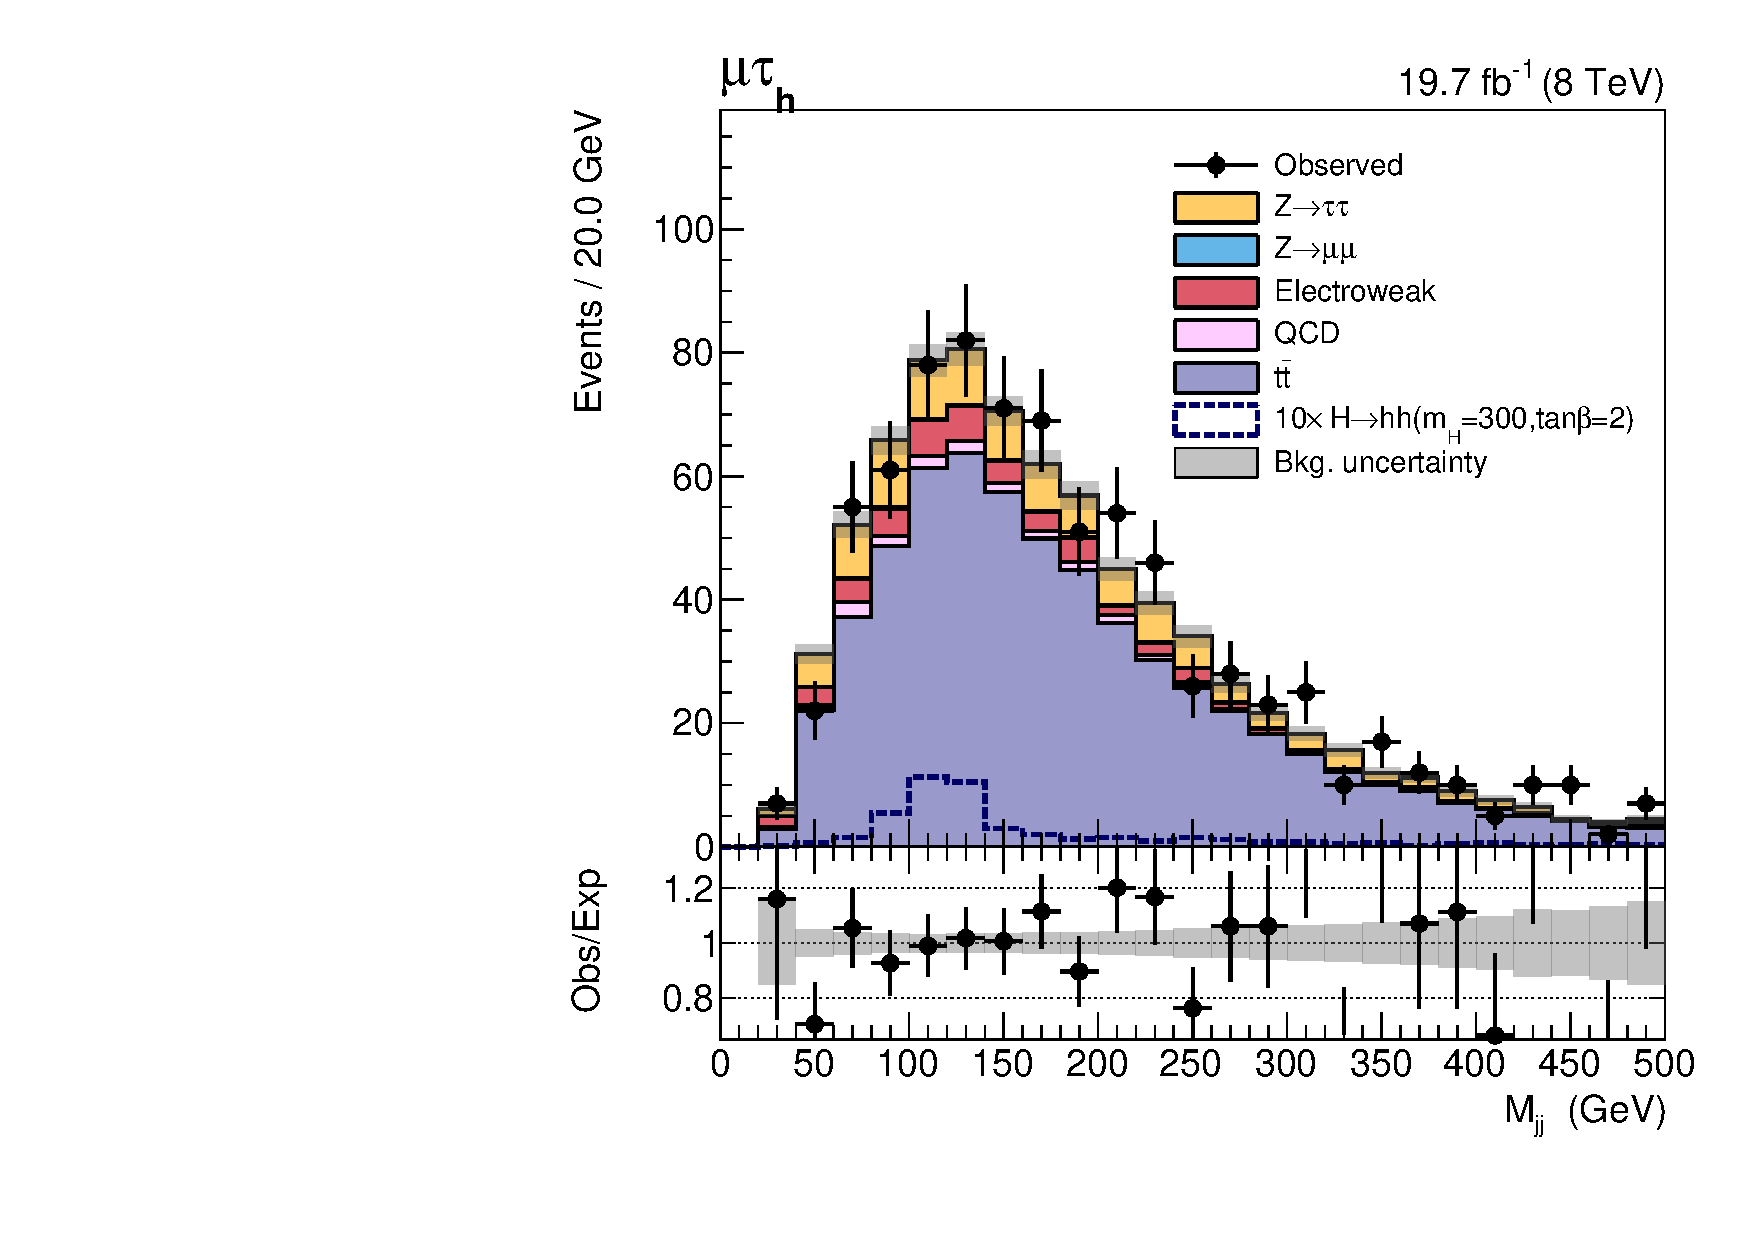
\includegraphics[width=0.5\textwidth]{Hhh/Plots/mjj_2jet2tag_mt_2012.pdf}}
\subfloat[$m_{jj}$ (\etau channel)]{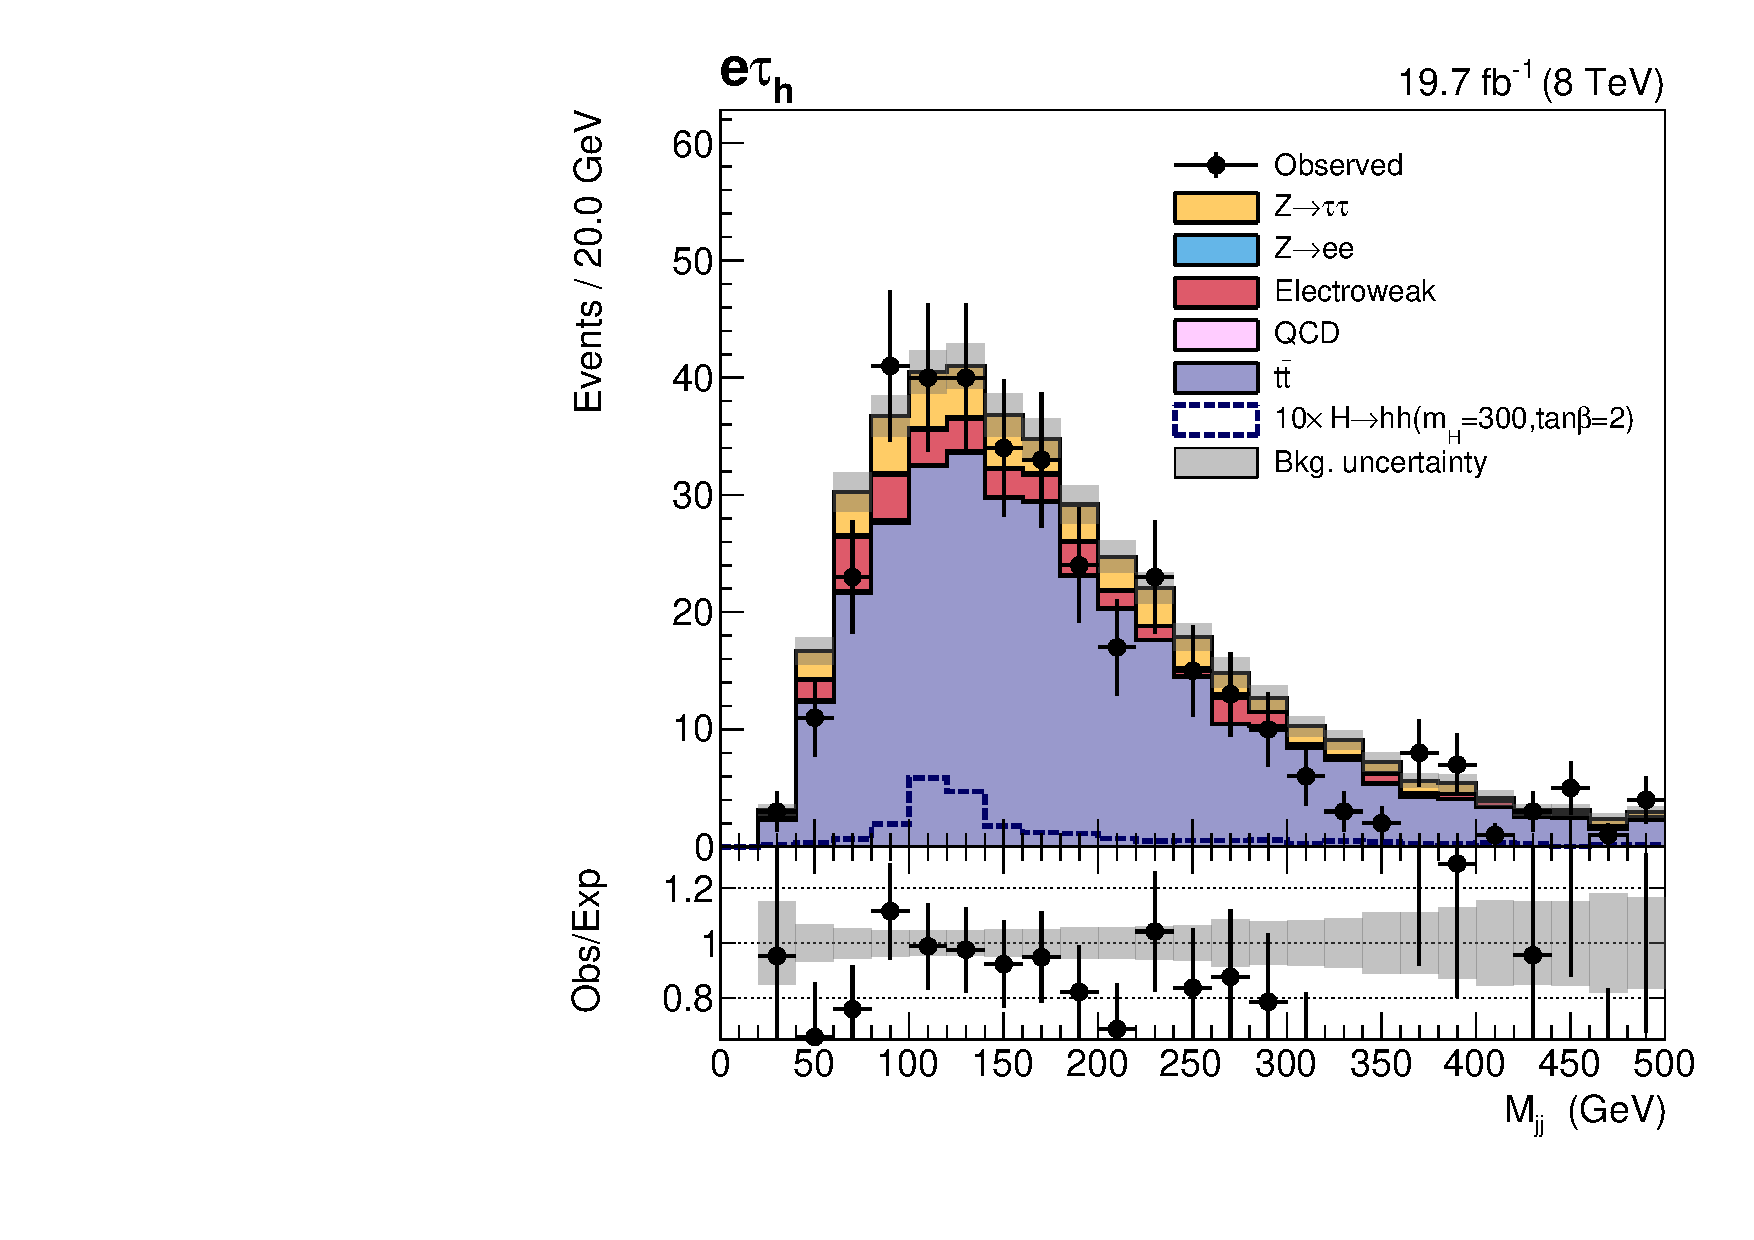
\includegraphics[width=0.5\textwidth]{Hhh/Plots/mjj_2jet2tag_et_2012.pdf}}
\end{center}
\caption{Reconstructed di-\Pgt invariant mass (top) and di-jet invariant mass (bottom) in the 2jet-2tag category of the \mutau (left) and \etau (right)
channels. The signal for a heavy Higgs boson H with mass \mH = 300 GeV at \tanb=2 in an MSSM scenario, enlarged by a factor 10, is overlaid on the figures.
One can see that this signal peaks at around 125 GeV.}
\label{fig:Hhh_selection_masscuts}
\end{figure}

\section{Data to Monte Carlo correction factors}
\label{sec:hhh_datamc}
Monte Carlo samples are used for the estimation of some of the backgrounds and the signal, 
and it is therefore important to correct for any mismodelling. The data to Monte Carlo
correction factors used for this are estimated in dedicated control regions.

A reweighting is applied to make the pile--up distribution in Monte Carlo
match the distribution observed in data.DESCRIPTION

Data and Monte Carlo identification, isolation, and trigger efficiencies
are measured for electrons, muons and hadronic taus. The difference between
the efficiencies in data and Monte Carlo are applied to Monte Carlo events as a
scale factor $SF = \frac{\epsilon_{\text{Data}}}{\epsilon_{\text{MC}}}$.

For electrons and muons, these scale factors are measured using a 
tag--and--probe method using \Zeenog and \Zmmnog events, respectively.
The hadronic taus identification, isolation and trigger efficiencies
are measured via a similar method that makes use of
$Z\rightarrow\Pgt\Pgt\rightarrow\Pgm\Pgt_{h}$ events.

FIXME: Tau es?

FIXME: top pt reweighting
FIXME: ttbar scale factor

In the \etau channel a data to Monte Carlo scale factor is applied
to the \Zee background, to correct for differences in the $e\rightarrow\Pgt_{h}$
fake rate between data and MC. DERIVED HOW

To correct for the difference in b--tagging efficiency and light jet mis--tagging
rates between data and Monte Carlo \pT and $\eta$ dependent scale factors are 
derived using the method described in \cite{BTV8TeV}. There are separate scale factors for 
b-/c- jets and light jets. There are multiple possible ways to apply these
scale factors, for this analysis this is done through a promote/demote method.

In this method a demotion or promotion probability is assigned to every
jet as in equation \ref{eqn:promotedemote}.

\begin{align}\label{eqn:promotedemote}
&P(\text{demote}) = 1 - SF \text{  for SF < 1 }  \notag \\
&P(\text{promote}) = \frac{(SF - 1)(\epsilon_{\text{MC}}-1)}{SF} \text{    for SF > 1}
\end{align}.

In this equation $SF$ is the scale factor mentioned above, and $\epsilon_{\text{MC}}$ is
the b--tagging efficiency in Monte Carlo events for the type of jet (light, b- or c-)
in consideration.



\section{Discriminating variable}
\label{sec:hhh_discr}
The variable of interest in this analysis is the mass of the heavy Higgs boson H. This can be
reconstructed as the 4--body mass of the two jets and the two taus, however
a more accurate result can be obtained by using a kinematic fitting 
procedure that makes use of the 125 GeV mass constraint on the di--tau and
di--jet candidates. 

In a kinematic fit constraints are made on the event kinematics, in the
case of this analysis these constraints are
$m(\Pgt_{1},\Pgt_{2}) = m_{h} = 125 $GeV and
$m(b_{1},b_{2}) = m_{h} = 125 $ GeV.
The kinematic observables related to the hadronic taus and jets
are varied within their uncertainties to fulfill these 
constraints. A $\chi^2$ cost term is introduced for each
observable that is varied with respect to the measurement,
the aim of the fit is to minimise this.

For b-jets, the reconstructed direction in $\eta$ and $\phi$ is 
assumed to be measured accurately in comparison with their energy.
Therefore only the energy is varied in the fit. In addition, we assume
that uncertainties in the energy measurement directly translate to
uncertainties in the momentum measurement, therefore $\vec{\beta} = \vec{p}/E$ is
also kept constant. 

Before the fit, from the mass constraint we have (equation \ref{eqn:kinfit_prefit})

\begin{align}\label{eqn:kinfit_prefit}
m_{h}^2 &= E_{h}^2 - \vec{p_{h}}^2 = (E_{b1}+E_{b2})^2 - (\vec{p_{b1}} + \vec{p_{b2}})^2 \notag\\
& = 2E_{b1}E_{b2} + m_{b1}^2 +m_{b2}^2 - 2\vec{p_{b1}}\vec{p_{b2}} \notag\\
& = m_{b1}^2 +m_{b2}^2 - 2E_{b1}E_{b2}(1-\vec{\beta_{b1}}\vec{\beta_{b2}})\notag\\
&\Rightarrow (1-\vec{\beta_{b1}}\vec{\beta_{b2}}) = \frac{m_h^2 - m_{b1}^2 - m_{b2}^2}{2E_{b1}E_{b2}}
\end{align}

When varying the energy of the first jet in the fit, equation \ref{eqn:kinfit_prefit} can be 
rewritten to derive an expression for the updated energy of the second jet. Using $\mathcal{A} = (1-\vec{\beta_{b1}}\vec{\beta_{b2}})$ 
and equation \ref{eqn:gamma_def}:

\begin{equation}\label{eqn:gamma_def}
\gamma = \frac{1}{1-\beta^2} \Rightarrow \gamma^2 = \frac{1}{1-\beta^2} = \frac{1}{1-p^2/E^2} = \frac{E^2}{m^2}
\end{equation}

We get:

\begin{align}\label{eqn:kinfit_variation}
m_h^2 &= m_{b1}^2 + m_{b2}^2 - 2E_{b1}E_{b2}(1-\vec{\beta_{b1}}\vec{\beta{b2}}\notag\\
&= m_{b1}^2 +\frac{E_{b2,fit}^2}{\gamma_{b2}^2} +2\mathcal{A}E_{b1}E_{b2,fit}\notag\\
\Rightarrow E_{b2}^{fit}& = \frac{(-2E_{b1}\mathcal{A} + \sqrt{4E_{b1}^2\mathcal{A} - 4(m_{b1}^2-m_{h}^2)\gamma_{b2}^{-2}})\gamma_{b2}^2}{2}\notag\\
&= E_{b1}\mathcal{A}\gamma_{b2}^2+\sqrt{E_{b1}^2\mathcal{A}\gamma_{b2}^4 - (m_{b1}^2 - m_{h}^2)\gamma_{b2}^2}\notag\\
&\Rightarrow E_{b2}^{fit} = E_{b1}\mathcal{A}\gamma_{b2}^2(-1 + \sqrt{1+\frac{m_{h}^2 - m_{b1}^2}{E_{b1}^2\mathcal{A}\gamma_{b2}^2}}\\
\end{align}

The fitting procedure additionally modifies the masses of the b-jets as (equation \ref{eqn:kinfit_bjetmass})
\begin{equation}\label{eqn:kinfit_bjetmass}
m_{b_{1,2}}^{fit} = m_{b_{1,2}}\frac{E_{b_{1,2}}^{fit}}{E_{b_{1,2}}}
\end{equation}

For each b-jet a $\chi^2$ term is calculated as $\chi_{b1,2}^2 = \frac{E_{b1,2}^{fit}-E_{b1,2}^{meas}}{\sigma_{b1,2}}$.

For taus only the visible decay products are measured. Assuming the visible decay products of the \Pgt point in 
the same direction as the \Pgt, a similar procedure as for the b-jets can be employed to constrain the mass of the second tau
when varying the mass of the first tau in the fit. The masses of the taus are kept fixed at $m_{\Pgt}$ throughout the procedure.

Due to the missing energy associated with the \Pgt decays, additional constraints
on the fit have to be used to reconstruct the correct tau energies. This is done by 
enforcing that the heavy Higgs boson recoil from the fit is close to the reconstructed recoil.

The measured recoil is (equation \ref{eqn:kinfit_recoilmeas})

\begin{equation}\label{eqn:kinfit_recoilmeas}
\vec{p_{\text{T,recoil}}}^{\text{meas}} = -\vec{p_{\text{T,H}}}^{\text{meas}} = -\vec{p_{\text{T,miss}}}^{\text{meas}} - \vec{p_{\text{T},b_{1}}}^{\text{meas}} - \vec{p_{\text{T},b_{2}}}^{\text{meas}} - \vec{p_{\text{T},\Pgt_1^{\text{vis}}}}^{\text{meas}} - \vec{p_{\text{T},\Pgt_2^{\text{vis}}}}^{\text{meas}}
\end{equation}

With the recoil from the fit (equation \ref{eqn:kinfit_recoilfit})
\begin{equation}\label{eqn:kinfit_recoilfit}
\vec{p_{\text{T,recoil}}}^{fit} = -\vec{p_{\text{T,H}}}^{fit} = - \vec{p_{\text{T},b_{1}}}^{fit} - \vec{p_{\text{T},b_{2}}}^{fit} - \vec{p_{\text{T},\Pgt_1}}^{fit} - \vec{p_{\text{T},\Pgt_2}}^{fit}
\end{equation}

A $\chi^2$ corresponding to the agreement between the fitted and measured recoil is reconstructed as (equation \ref{eqn:kinfit_recoilchi2})

\begin{equation}\label{eqn:kinfit_recoilchi2}
\chi^2_{\text{recoil}} = (\vec{p_{\text{T,recoil}}}^{\text{fit}} - \vec{p_{\text{T,recoil}}}^{\text{measured}})^T V_{\text{recoil}}^{-1}(\vec{p_{\text{T,recoil}}}^{\text{fit}} - \vec{p_{\text{T,recoil}}}^{\text{measured}})
\end{equation}

where the covariance matrix $V_{\text{recoil}}$ of the recoil vector is estimated as in equation \ref{eqn:kinfit_recoilcov} from the covariance matrices of the b-jets and
the covariance matrix of the missing transverse momentum. The latter is estimated in the process of determining the MVA \MET (OBJECT RECO),
while the covariance matrices of the b-jets can be written in terms of position, momentum and resolution of the b-jets. 

\begin{equation}\label{eqn:kinfit_recoilcov}
V_{\text{recoil}} = V_{\vec{p_{\text{T,miss}}}} - V_{b_{1}} - V_{b_2} 
\end{equation}

The total $\chi^2$ term that needs to be minimised in the fit can then be written as (equation \ref{eqn:kinfit_chitot})

\begin{equation}\label{eqn:kinfit_chitot}
\chi^2 = \chi^2_{b_1} + \chi^2_{b_2} + \chi^2_{\text{recoil}}
\end{equation}

The result of the kinematic fit are the tau and b-jet 4-vectors with their energies and momenta
set to the best fit values found for them in the fit. These can then be added together to find
the mass of the heavy Higgs boson as reconstructed by the kinematic fit.

As illustrated in figure \ref{fig:kinfitvsmjj} the use of the kinematic fit greatly
improves the resolution of the reconstructed heavy Higgs mass in signal events, when 
compared with the simple 4-body mass reconstruction. It also shifts the mean of the
distribution closer to the true value. From the right hand side of
figure \ref{fig:kinfitvsmjj} one can see that the mass distribution for
background events is less affected by the kinematic fit, although due to the
invariant mass constraint the minimum of the reconstructed mass distribution
is forced to 250 GeV.

\begin{figure}[h!]
\begin{center}
\subfloat[Signal]{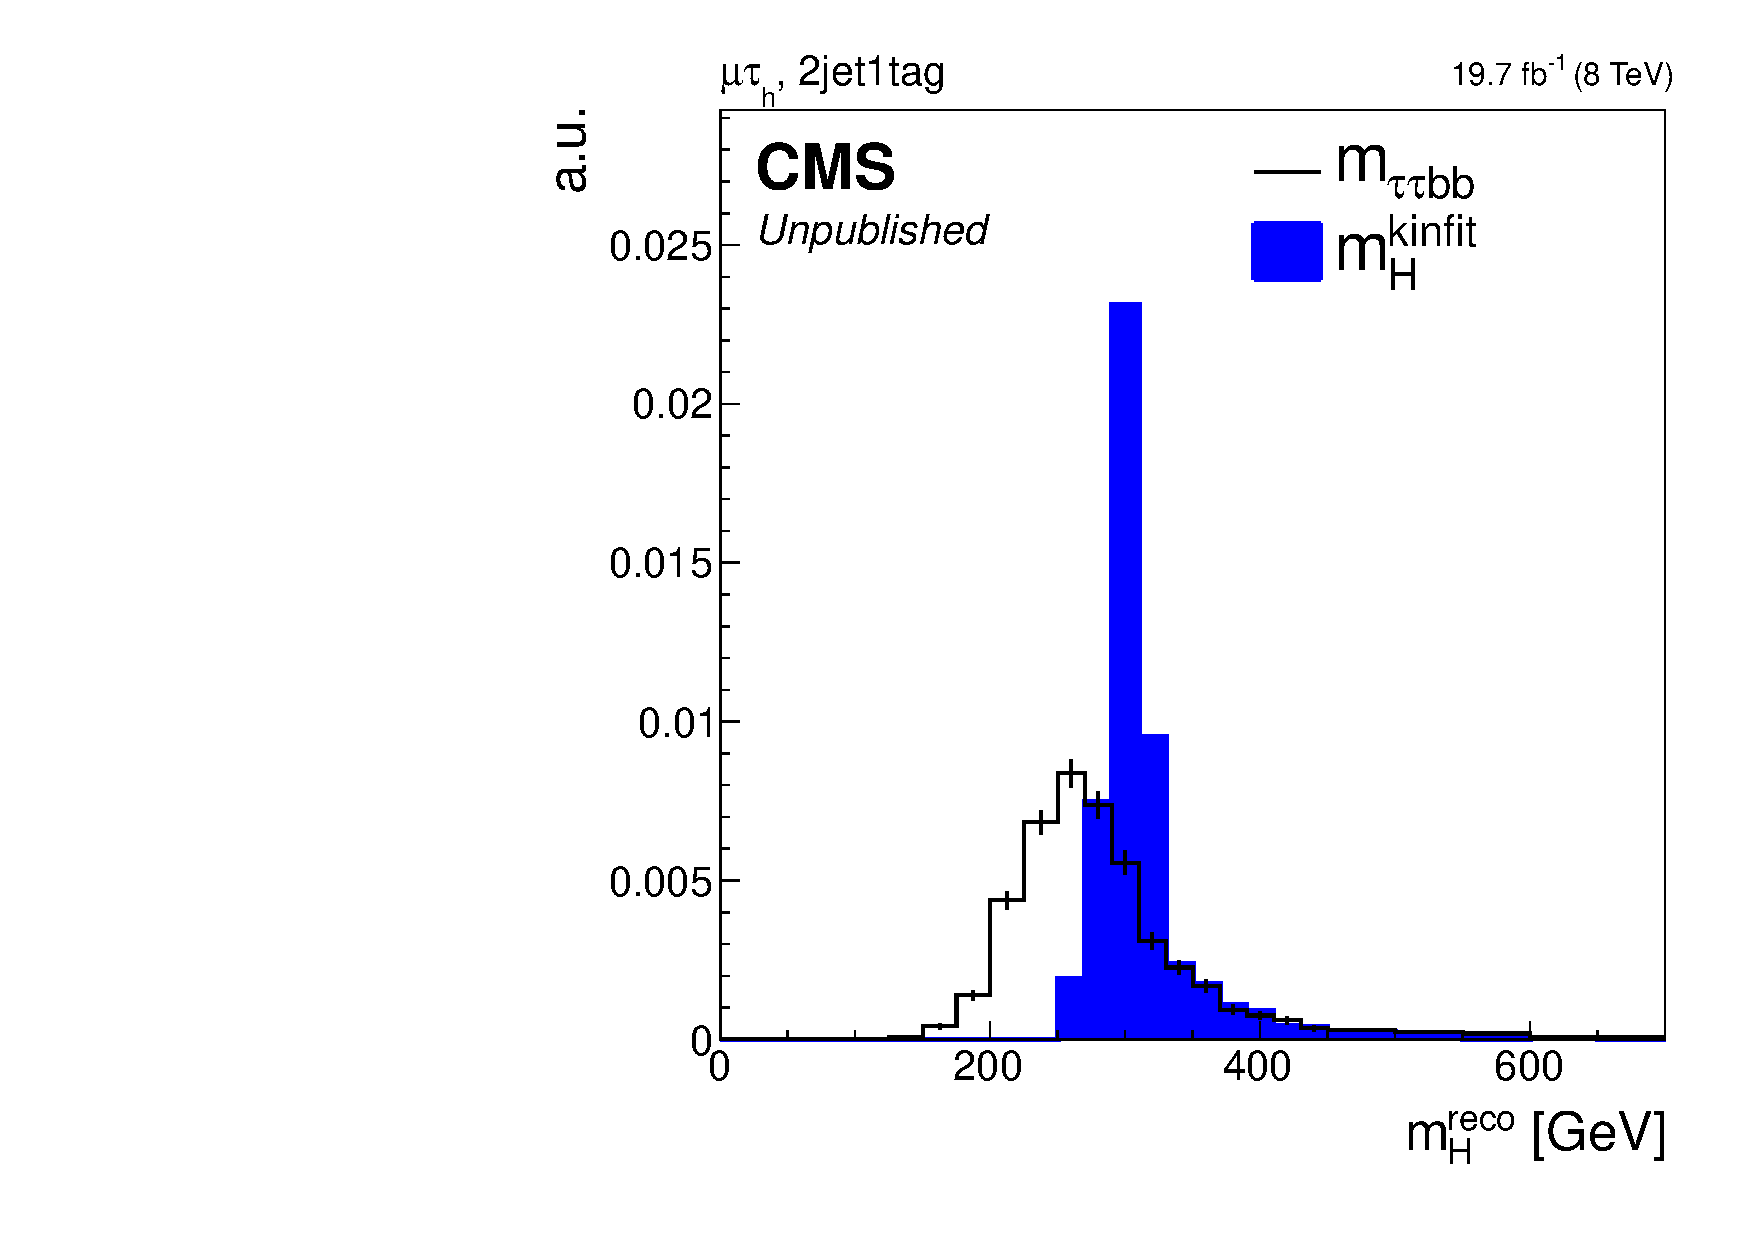
\includegraphics[width=0.5\textwidth]{Hhh/Plots/CMS-HIG-14-034_Figure-aux_020.pdf}}
\subfloat[\ttbar background]{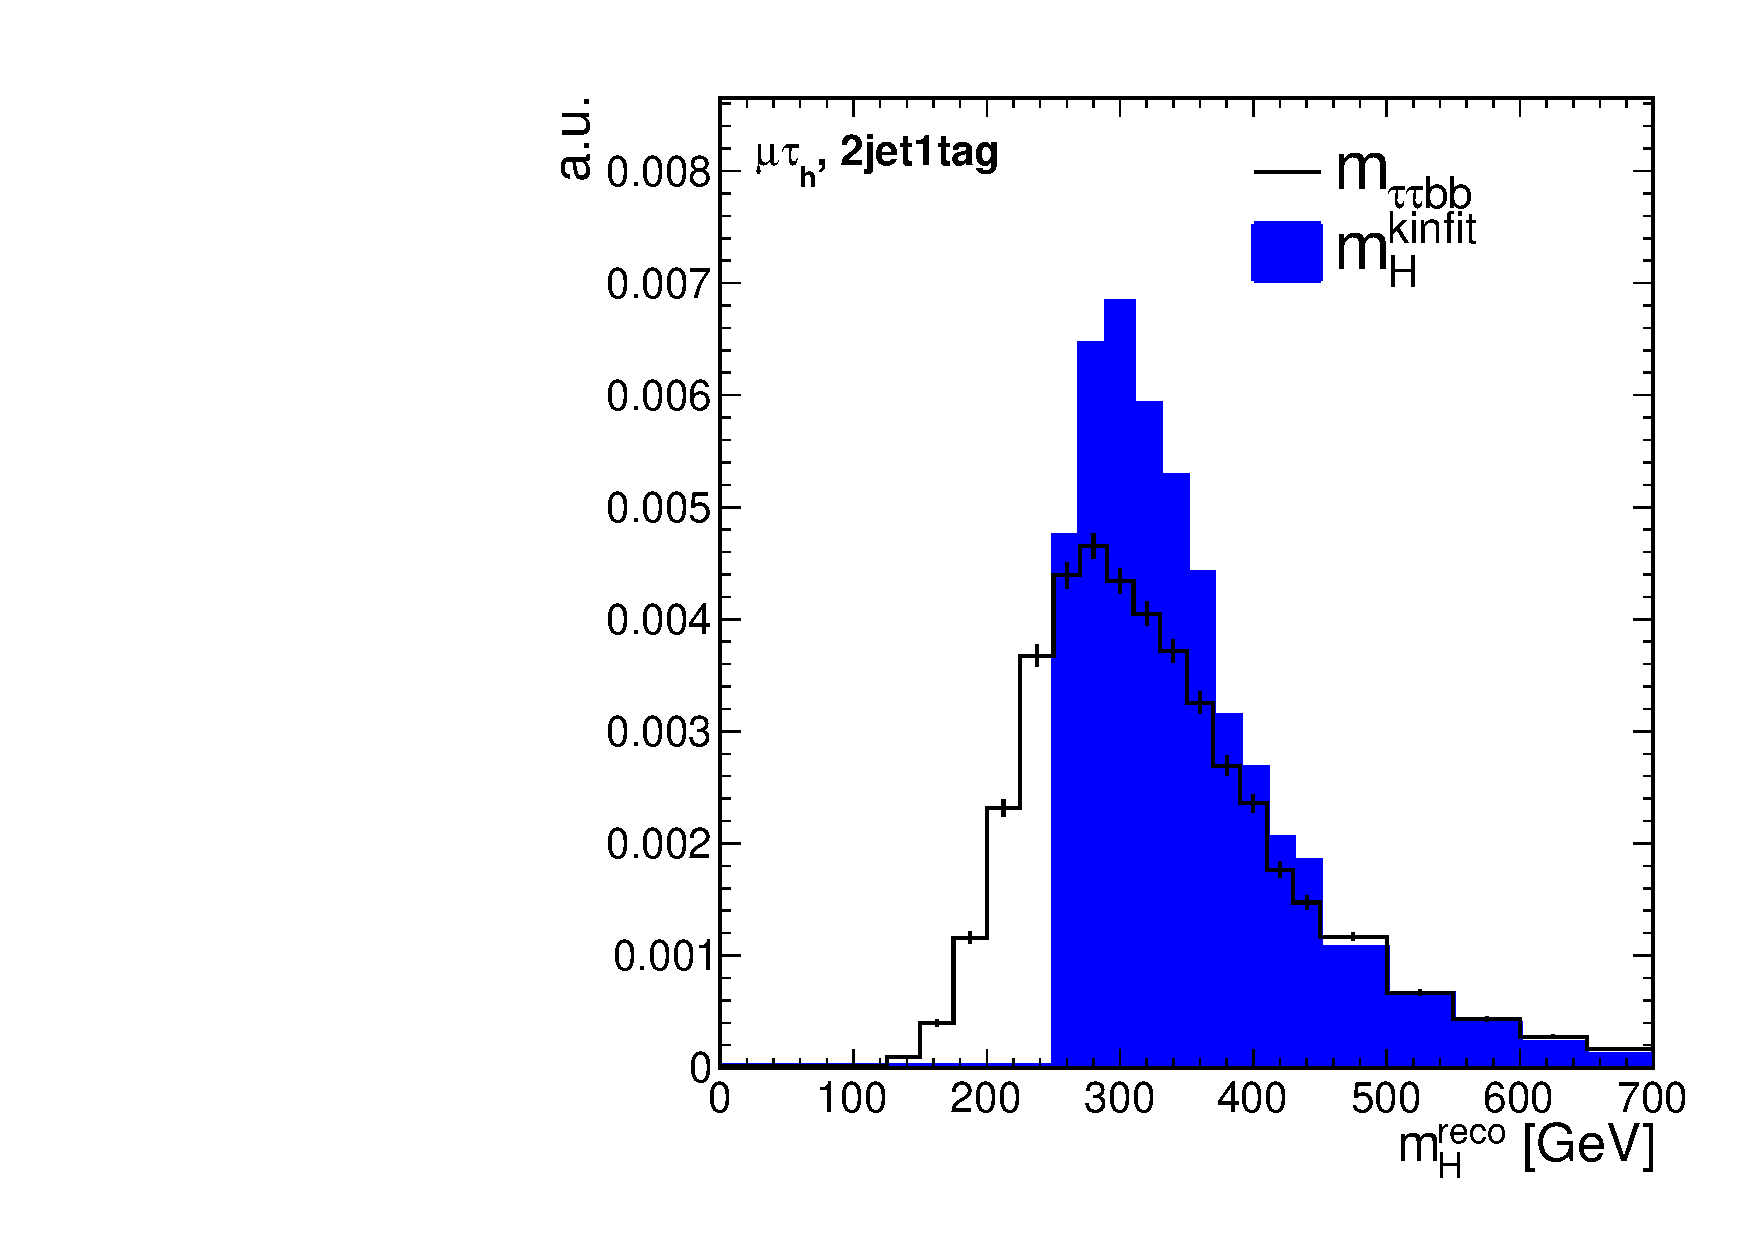
\includegraphics[width=0.5\textwidth]{Hhh/Plots/mHvsmttbb_ttbar.pdf}}
\end{center}
\caption{Comparison of the reconstructed heavy Higgs mass using the kinematic fit (blue) and
4-body mass without use of the kinematic fit (black) in signal events with $m_{H} = 300 $GeV (left) and \ttbar background events (right) in 
the 2jet-1tag category of the \mutau channel. The kinematic fit greatly improves the resolution and 
accuracy of the mean of the mass distribution in signal events. \cite{HIG-14-034-additional}}%FIXME plots need to be remade as the bkg one was never released
%on the public twiki so can't have the CMS label on
\label{fig:kinfitvsmjj}
\end{figure}


\section{Background estimation}
\label{sec:hhh_backgrounds}
To estimated the shape and yield of backgrounds in this analysis, data--driven techniques are
used where possible. 

\subsection{\texorpdfstring{\Ztautau}{Z to tau tau}}
\label{sec:hhh_backgrounds_ztt}
The \Ztautau background is estimated using the embedded samples
described in section \ref{sec:hhh_datasets}. To estimate the 
yield of \Ztautau in each category, the total
yield after the initial event selection (before subdividing into categories) as
estimated in \Ztautau Monte Carlo samples is scaled by the efficiency with which 
such events pass the category selection in the embedded sample. The shape of
the \Ztautau background is taken from the embedded sample after applying the full
category selection. The contamination from \ttbar backgrounds in the embedded
sample is accounted for by subtracting this contamination, as evaluated using
the dedicated \ttbar embedded samples, from the \Ztautau background.

\subsection{\texorpdfstring{\ttbar}{ttbar}}
Both the \ttbar shape and normalisation are estimated using Monte Carlo samples.
These are checked against data in dedicated control regions. One such control
region uses the \emu final state of the taus. In this control region
a data-to-Monte Carlo scale factor is estimated and applied to the yield estimate from Monte Carlo.

\subsection{\texorpdfstring{\Wjets}{W + jets}}
\label{sec:hhh_backgrounds_wjets}
The \Wjets background is greatly reduced by requiring \mT to
be less than 30 GeV. To estimate the remaining contribution
from \Wjets in the signal region a sideband with \mT greater
than 70 GeV is used in the 2jet-0tag and 2jet-1tag categories.
Contributions from other backgrounds are subtracted 
from the data in this region, and a high \mT to low \mT
extrapolation factor is determined from the \Wjets Monte Carlo
samples. The yield in the signal region is then the other-background-subtracted
data yield in the high \mT region multiplied by this extrapolation factor.
In the 2jet-2tag, a slightly different high \mT sideband of 60-120 GeV is used 
to give larger statistics for the \Wjets estimate after other backgrounds are
subtracted. The method of extrapolating this yied estimate into
the signal region is otherwise analogous.

The \Wjets shape is taken from the Monte Carlo samples. To 
increase the statistics for this estimate, the b-tagging definition
in the 2jet-1tag and 2jet-2tag categories is loosened to the loose (instead of medium)
working point for the purposes of shape estimation.


\subsection{QCD}
\label{sec:hhh_backgrounds_qcd}
A fully data-driven method is used to estimate the QCD background. Data events
passing the signal region selection cuts, but requiring the di-tau pair to be
of the same sign, are used for this. Contributions from other backgrounds are 
subtracted. Because the contribution from opposite- and same-sign QCD are
not exactly the same an OS/SS ratio of 1.06 is measured using data in which
the electron/muon isolation requirement was inverted. 

For the 2jet-0tag and 2jet-1tag categories the yield is taken directly from
the same-sign subtracted data multiplied by the OS/SS ratio. In the 2jet-2tag
category the statistics are too low for this, so another sideband is defined
in which the electron/muon isolation requirement is inverted. This 
sideband is then used to determine an extrapolation factor from events
with 2 jets to events passing the 2jet-2tag category selection. This extrapolation
factor is then applied to a QCD estimate as described above, but using the 2-jet 
selection only, to obtain the yield in the 2jet-2tag category.

The shapes in all categories are taken from same-sign data with the electron/muon
isolation inverted. For the 2jet-1tag and 2jet-2tag categories, in addition to 
inverting the light lepton isolation requirements, the category definition
is loosened to obtain the shapes. For the purposes of QCD shape
estimation, jets are considered b-tagged if they pass a looser b-tagging
working point than the working point used elsewhere in the analysis.

\subsection{Other backgrounds}
\label{sec:hhh_backgrounds_other}
The remaining backgrounds of \Zellell, di-boson and single-top
events are small. Both shape and normalisation are
estimated using Monte Carlo samples.
 

\section{Systematic uncertainties}
\label{sec:hhh_uncs}
Two types of systematic uncertainties are considered: normalisation
uncertainties (which affect only the yield of a process), and shape
uncertainties (which affect both the yield and shape of a process). Section \ref{sec:hhh_results_extraction}
describes how these uncertainties are taken into account in the final result.

\subsection{Normalisation uncertainties}
\label{sec:hhh_uncs_norm}

\subsubsection*{Luminosity uncertainty}
The uncertainty on the luminosity measurement amounts to 2.6\% for data collected during
2012 (LUMI POG CITATION?). This uncertainty is applied to all processes in which
the normalisation is estimated using MC samples.

\subsubsection*{Identification, isolation and trigger efficiencies}
A systematic uncertainty due to the uncertainty in efficiency measurements
for the leptons is derived by combining the uncertainties on these measurements
in quadrature. For electrons and muons this leads to a 2\% uncertainty, for hadronic taus a 6\% 
uncertainty is measured on the tau identification efficiency, with an additional uncertainty of 3 \% for
the \Pgt legs of the triggers. This uncertainty is applied to all processes for which
the normalisation is estimated using MC samples.

\subsubsection*{$e\rightarrow\Pgt_{h}$ and $\mu\rightarrow\Pgt_{h}$ fake rates}
The uncertainty on both the $e\rightarrow\Pgt$ fake rate measurement and the
$\mu\rightarrow\Pgt$ fake rate measurement is 30\%. The central value of the $\mu\rightarrow\Pgt$
fake rate is close to 1, which is why it is not applied, but the uncertainty is 
taken into account FIXME check if this is true!


\subsubsection*{B-tag scale factors}
The b-tag scale factors are varied within their uncertainties to determine the effect
on the yields of each process. Both a b-tagging uncertainty and a fake mis-tagging
uncertainty are obtained by considering the percentage by which these backgrounds
change when the scale factors are varied within their uncertainty. The b-tagging
efficiency uncertainty amounts to 1-10\% for most processes in most categories, except for the 2jet-2tag
category where a 70\% uncertainty applies to the W background. Due to the nature
of the estimation method, where other backgrounds are subtracted from the data to 
obtain a W estimate, and the presence of large amounts of \ttbar, a 10\% change in the \ttbar
yield can vary the W yield by such large amounts.
The b mistagging rate uncertainty varies between 1-5\% for all processes in all channels.

\subsubsection*{\MET resolution and response}
Uncertainties on the \MET resolution and response are estimated by varying
the recoil correction parameters within their estimated uncertainties. This 
leads to a 1-10\% uncertainty (depending on category and process)

\subsubsection*{Background normalisation}
\begin{itemize}
\item \Ztautau : the normalisation of the embedded samples attracts a 3.3\% uncertainty, which is derived
from combining the estimated normalisation uncertainty on the embedded samples themselves, and the uncertainty on the \ttbar embedded samples. In addition an uncertainty of 5-6\% for extrapolation from the inclusive selection to the category selection is applied.
\item \Zellell: As this is a very small background after requiring 2 jets, the uncertainty on this estimate is derived from the statistical uncertainty on the yield estimate, which varies between 20-90\%
\item \ttbar: the uncertainty on the \ttbar cross section is 10\%
\item di-boson and single top: the uncertainty on the di-boson and single-top cross section is 15\%
\item \Wjets: As the \Wjets yield is estimated from a high \mT sideband in data, the uncertainty on this yield estimate is primarily due to the statistics available in the control region, the uncertainty range sfrom 10\% in the 2jet-0tag cateogry to 100\% in the 2jet-2tag cateogry
\item QCD: The QCD normalisation uncertainty is obtained by adding the statistical uncertainty on the data-subtracted same-sign region in quadrature with the 10\% uncertainty on the OS/SS ratio. This yields a 20\% uncertainty in the 2jet-0tag category, a 40\% uncertainty in the 2jet-1tag category and a 60-100\% uncertainty in the 2jet-2tag category.
\end{itemize}

\subsection{Shape uncertainties}
\label{sec:hhh_uncerts_shape}

\subsubsection*{Tau energy scale}
The energy of hadronically decaying taus is varied up and down by its 3\% uncertainty. As this directly affects the kinematic fit mass distribution this uncertainty is then applied as a shape uncertainty.

\subsubsection*{Jet energy scale}
The uncertainties on the jet energy corrections are applied by shifting the jet energy up and down by the (\pT and $\eta$ dependent) uncertainty. Again, as this affects the shape of the kinematic fit mass distribution this uncertainty is applied as a shape uncertainty 


\section{\texorpdfstring{Overview of \AtoZhtolltautau}{Overview of A->Zh->lltautau}}
\label{sec:hhh_azh}
In this section a summary of the \AtoZhtolltautau analysis, which is combined with the 
analysis described so far for the purposes of model interpretations, is given.

The search for \AtoZhtolltautau also uses the full dataset collected by the CMS experiment during
the 2012 $p-p$ running period of the LHC. In this search the \mumu and \ee final states of the \PZ boson
and the \emu, \etau, \mutau and \tautau channels of the \htotautau decay, leading to a total of
eight final states. 

First the \PZ candidate is chosen as a pair of isolated electrons or muons, with opposite charge, and 
invariant mass of the pair between 60-120 GeV. In case there is more than one possible pair, the 
pair with invariant mass closest to the \PZ mass is chosen. The \htotautau decay is chosen by selecting
an oppositely charged pair of isolated leptons in the four channels mentioned earlier. To ensure no overlap
between different final states is possible, events with additional electrons or muons satisfying the
\pT and $\eta$ requirements are discarded.

To reject some of the backgrounds from misidentified leptons and \ZZ production, a requirement is made
on the scalar sum of the visible transverse momenta of the two $\tau$ candidates from the \htotautau decay.
This selection changes by final state and has been chosen to optimise the analysis sensitivity to an 
\AtoZh signal with \mA $= 220 - 350 $ GeV. Furthermore \ttbar events are discarded by rejecting
events with at least one b-tagged jet. 

Remaining backgrounds from \ZZ, triboson and \ttbar\PZ production are estimated using
Monte Carlo samples. Backgrounds from \PZ+jets %($\ell\ell\tautau$ channel) 
and \WZ+jets %($\ell\ell\mutau$ and $\ell\ell\etau$ channels) 
events, with at least one misidentified lepton, are estimated from control regions in data.

For signal extraction, the mass of the A boson \mA, reconstructed by combining the
4-vector of the \PZ candidate with the 4-vector of the \Ph -candidate,as obtained by using the 
\texttt{SVFit} algorithm. The expected and observed 95\% confidence level upper limits, for
all $\ell\ell\tau\tau$ final states combined, is shown in figure \ref{fig:AZhUpperLimits}

\begin{figure}[h!]
\begin{center}
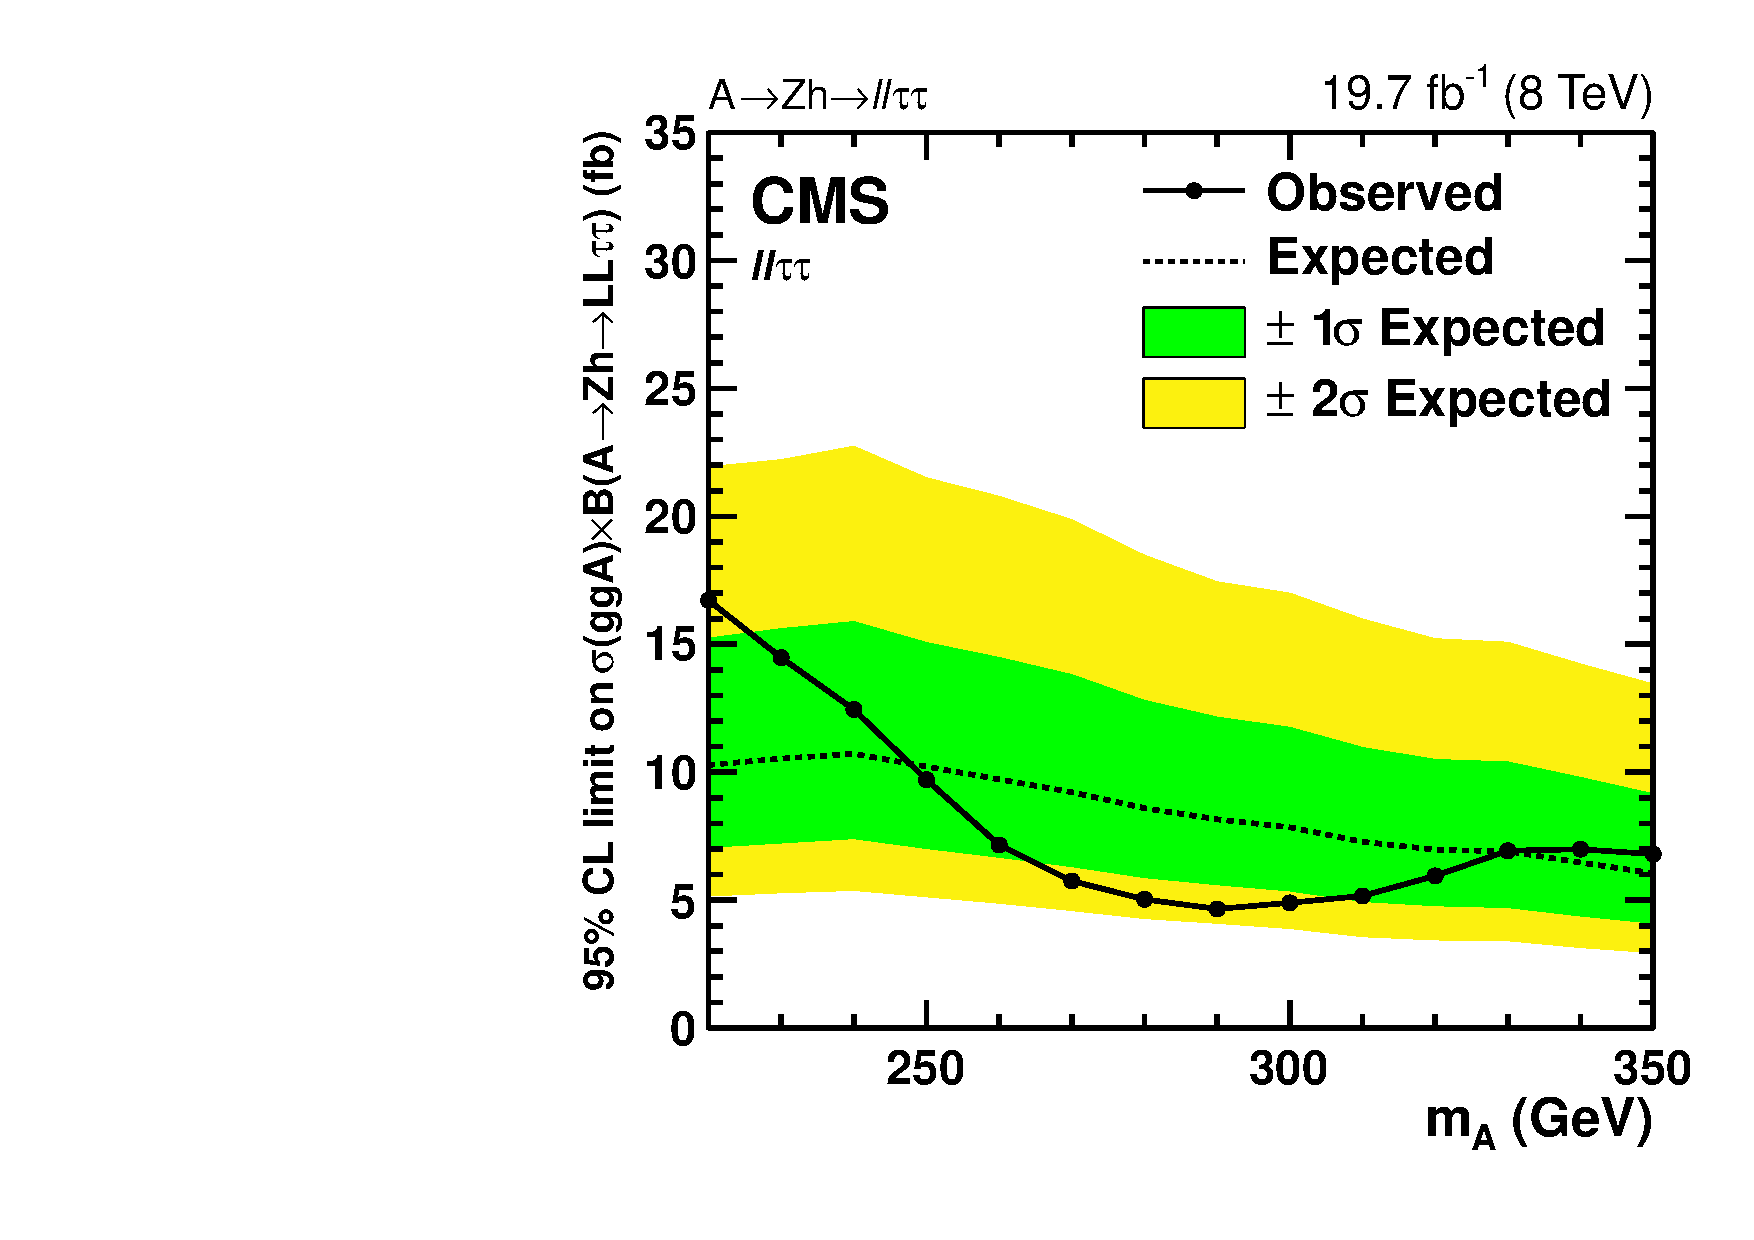
\includegraphics[width=0.85\textwidth]{Hhh/Plots/CMS-HIG-14-034_Figure_010-a.pdf}
\caption{The 95\% confidence level expected (dashed) and observed (solid)
upper limits on the $\sigma \times BR$ for the \AtoZhtolltautau process.
The green and yellow bands indicate the $\pm 1 \sigma $ and $2\sigma$
expectations \cite{CMS-HIG-14-034}.}
\label{fig:AZhUpperLimits}
\end{center}
\end{figure}



More detail on this analysis can be found in reference \cite{CMS-HIG-14-034}.




\section{Results}
\label{sec:hhh_results}

\subsection{Signal extraction}
\label{sec:hhh_results_extraction}

\subsection{Model-independent results}
\label{sec:hhh_results_modelindep}

The $m_{H}^{\text{kinfit}}$ distributions in the \mutau and \etau channel 
are shown in figures \ref{fig:hhh_results_mhkinfit_mutau} and \ref{fig:hhh_results_mhkinfit_etau} 
respectively.

\begin{figure}[h!]
\begin{center}
\subfloat[2jet-0tag]{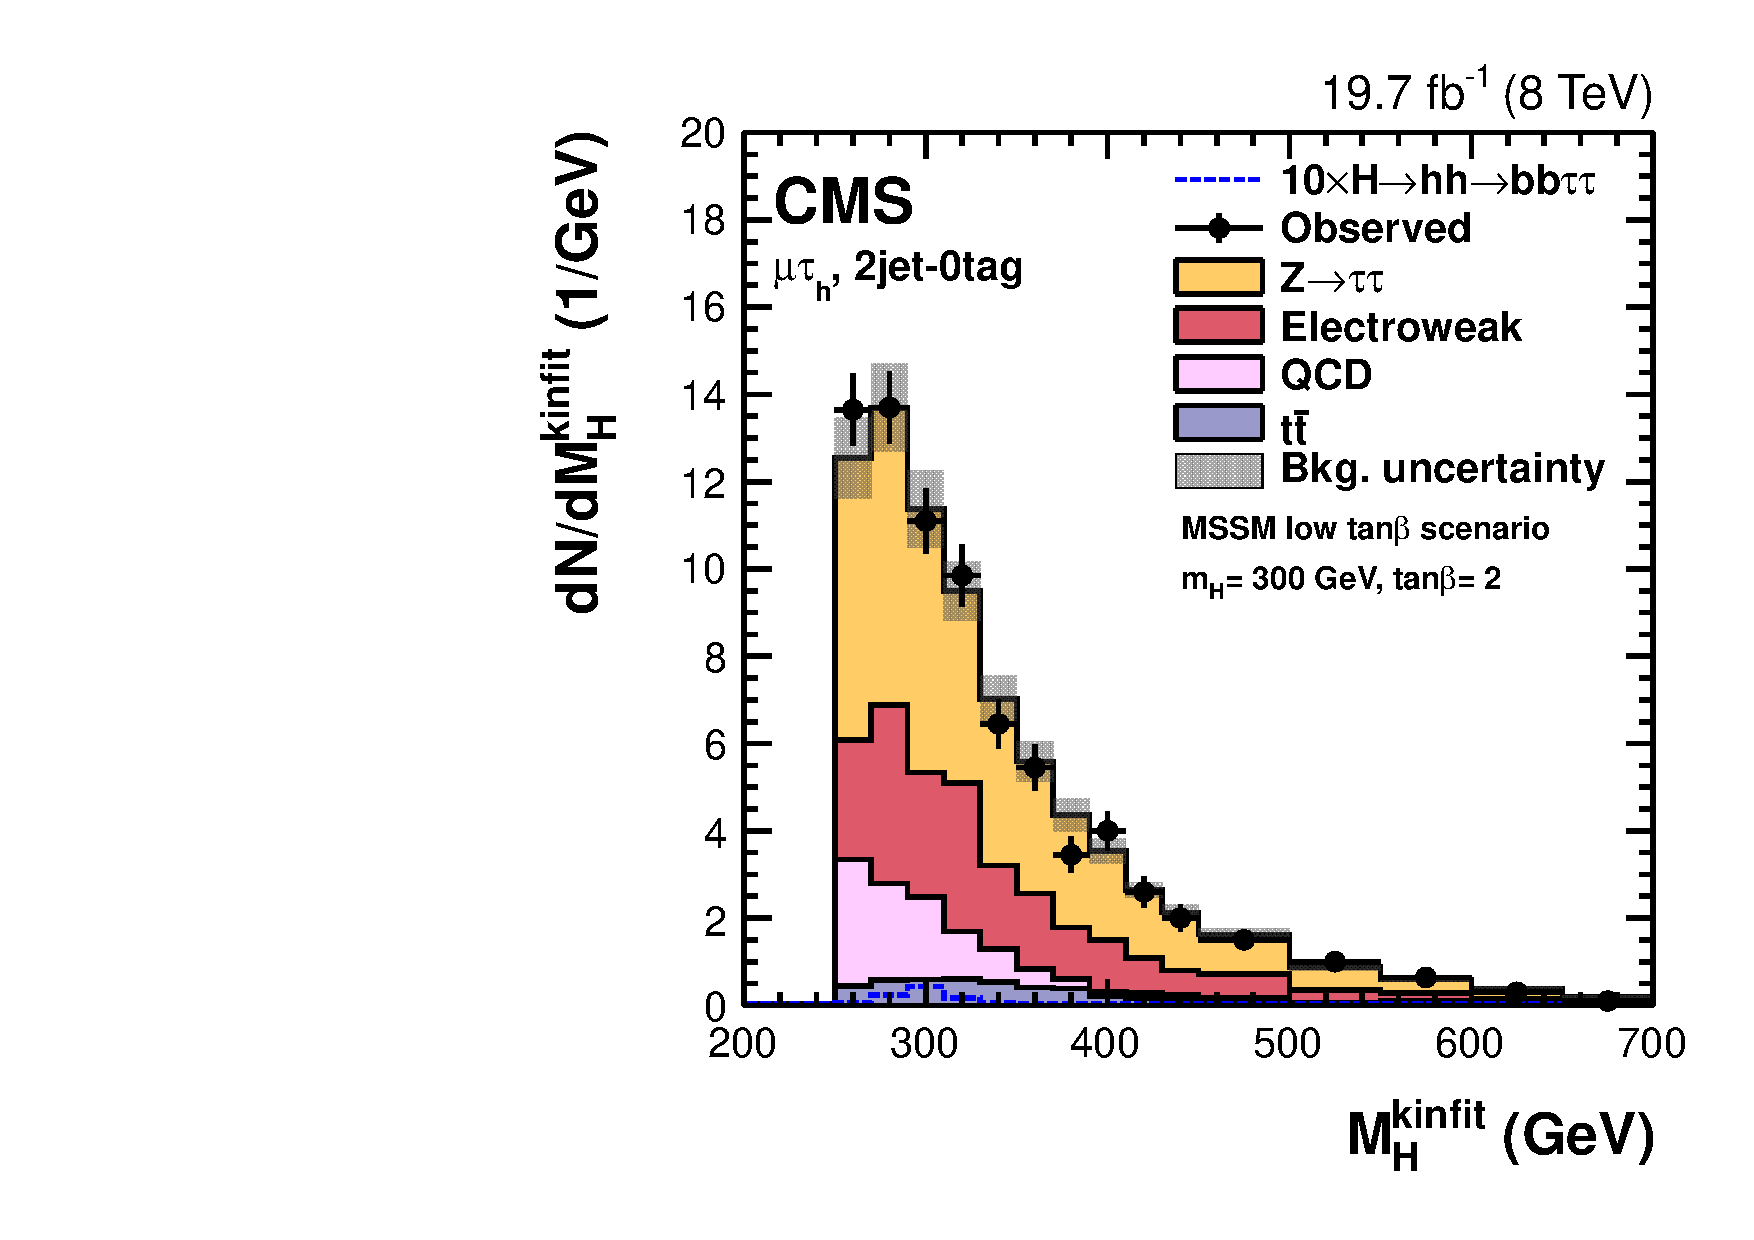
\includegraphics[width=0.5\textwidth]{Hhh/Plots/CMS-HIG-14-034_Figure_003-a.pdf}}
\subfloat[2jet-1tag]{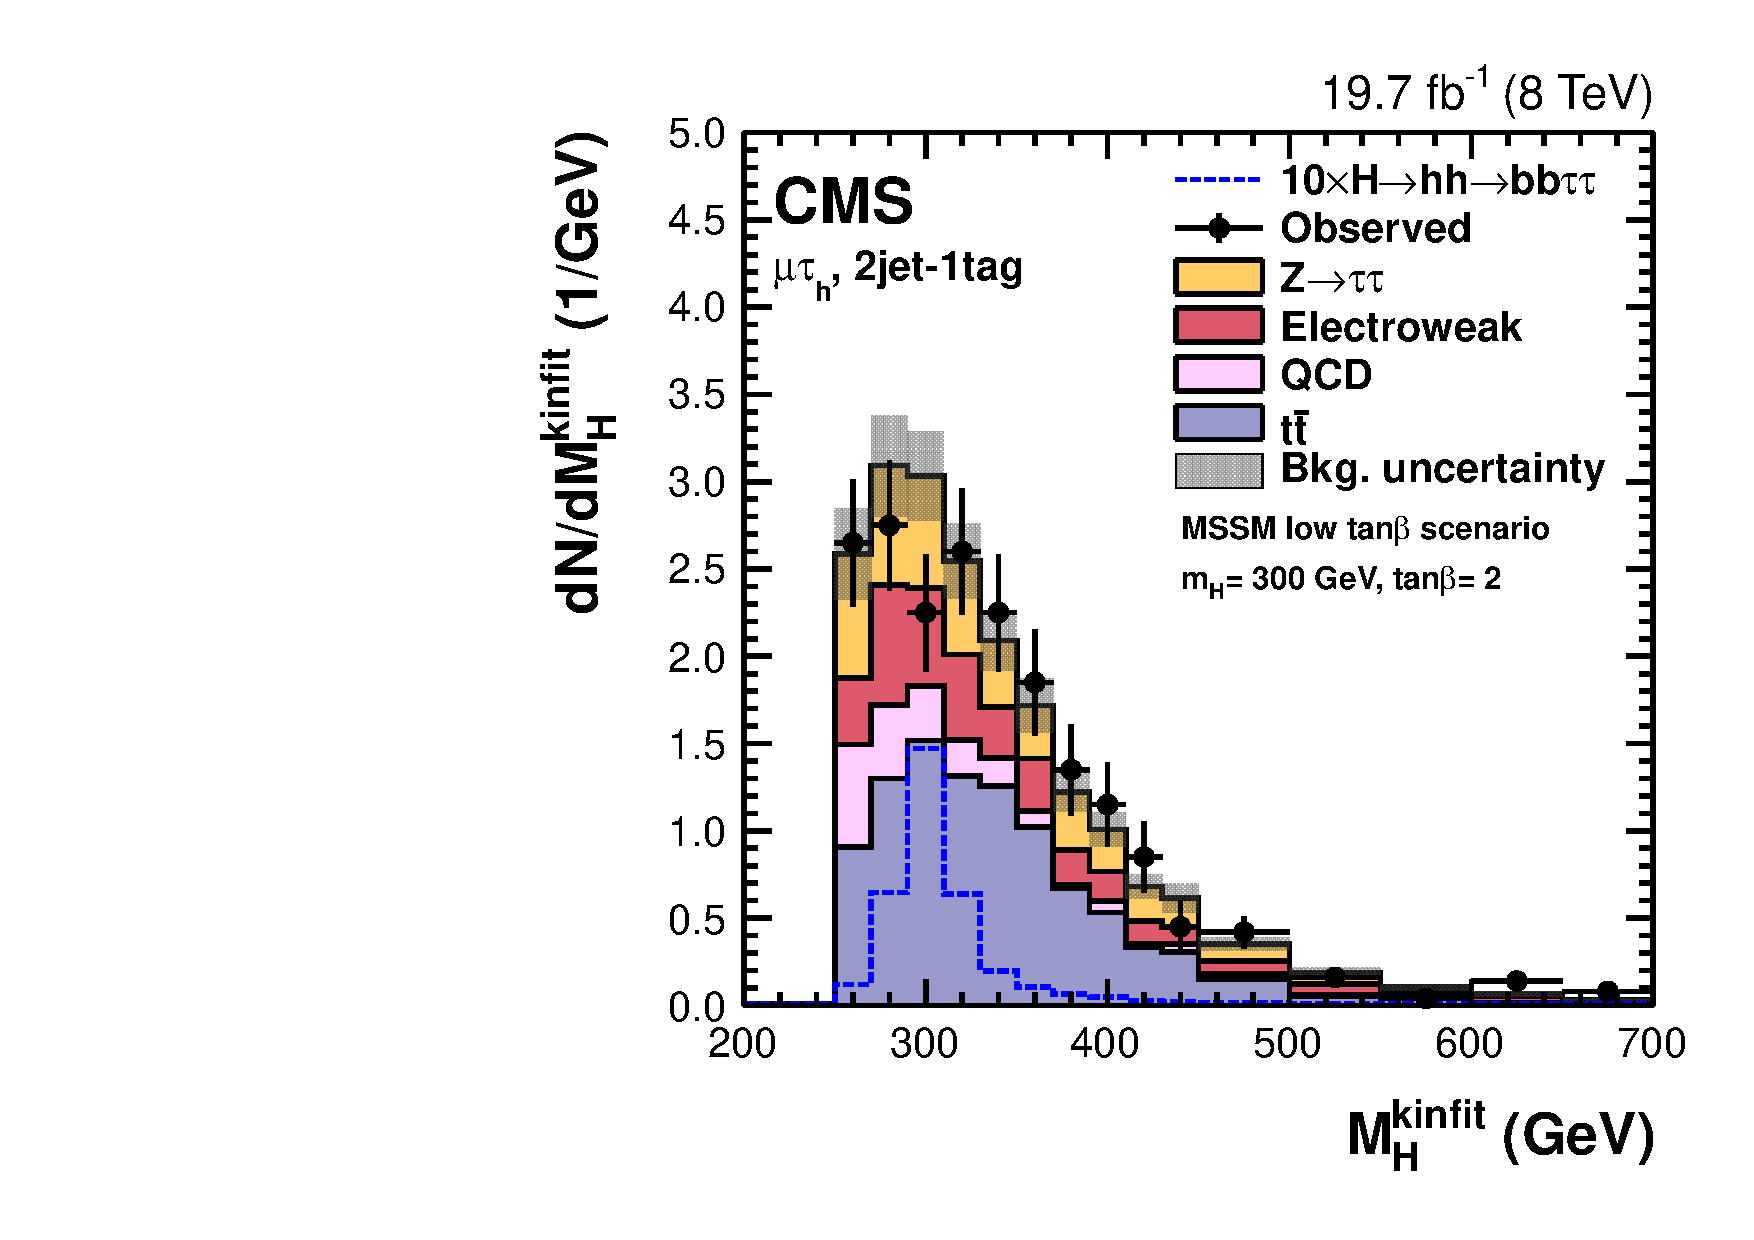
\includegraphics[width=0.5\textwidth]{Hhh/Plots/CMS-HIG-14-034_Figure_003-b.pdf}}~\\
\subfloat[2jet-2tag]{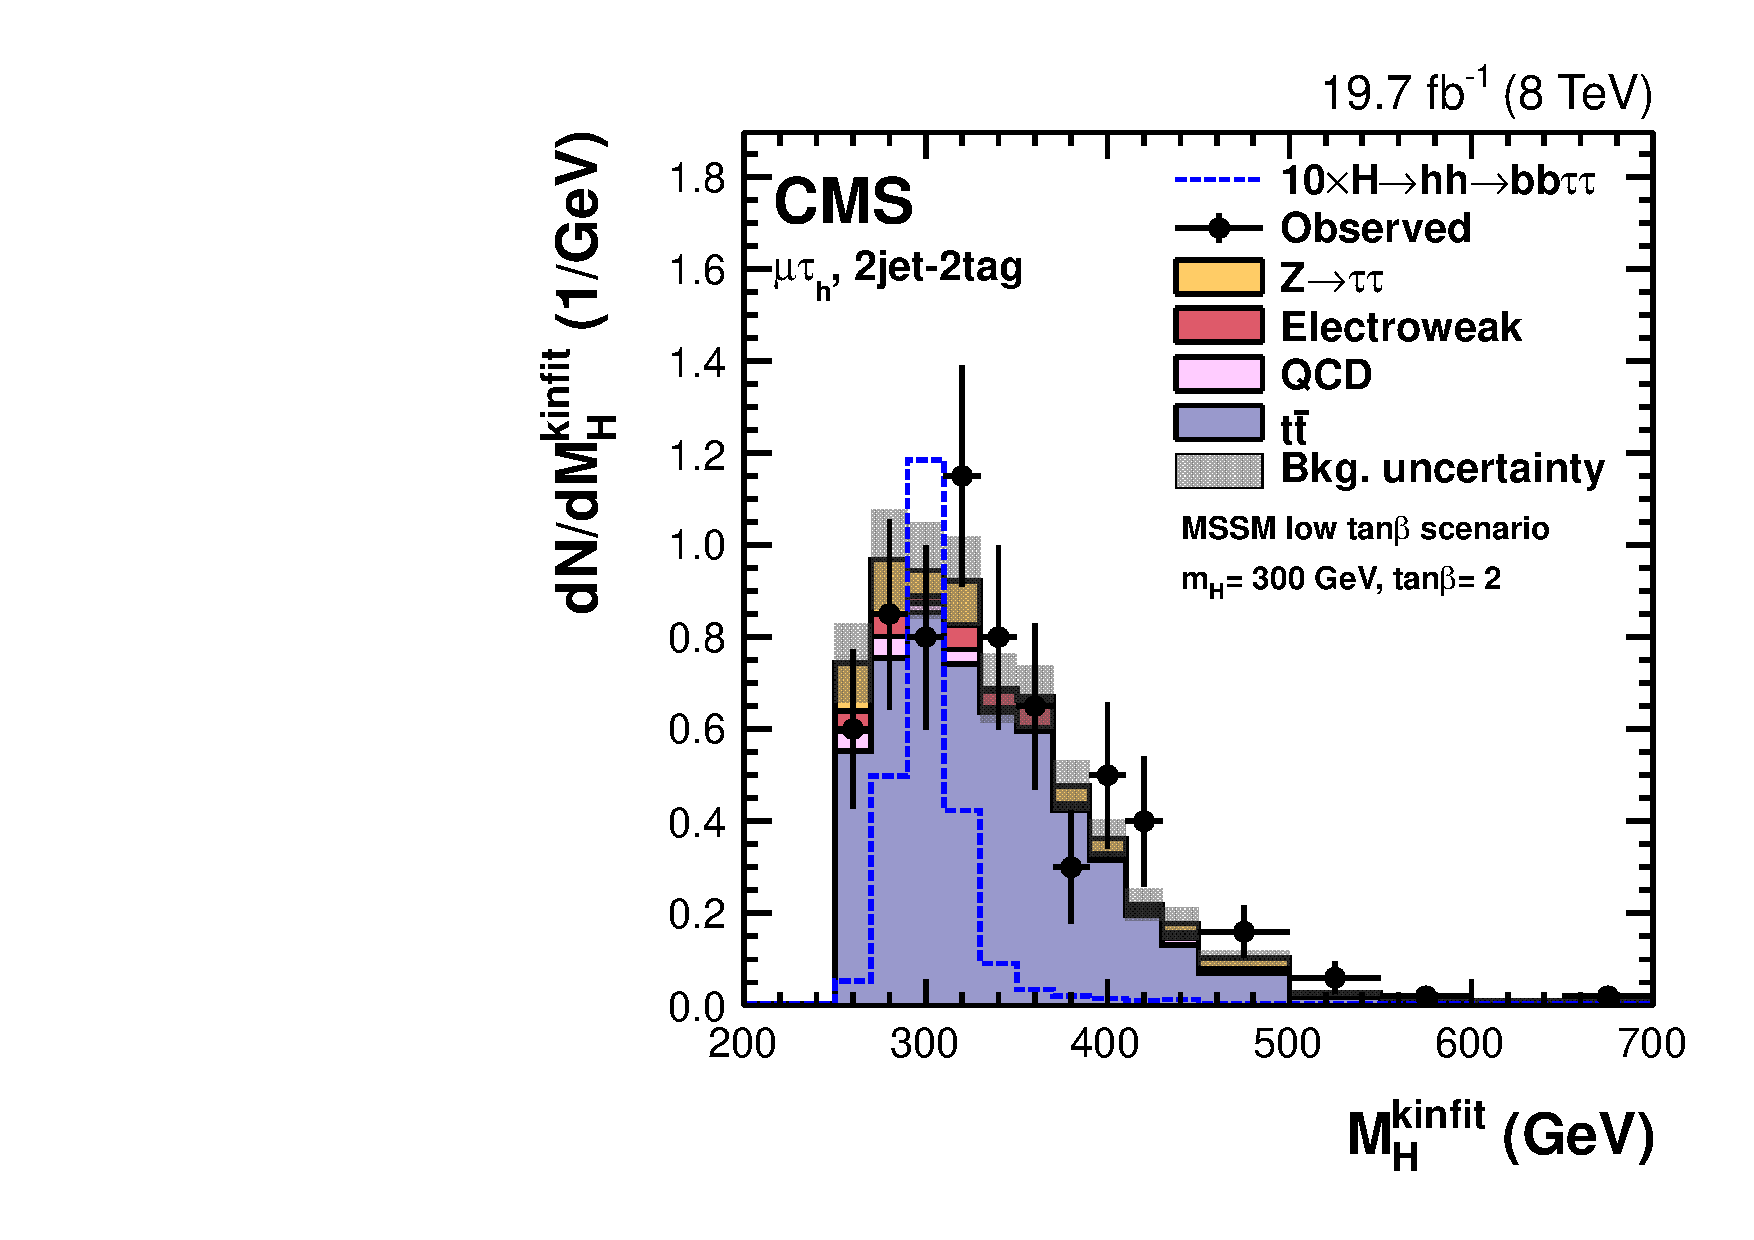
\includegraphics[width=0.5\textwidth]{Hhh/Plots/CMS-HIG-14-034_Figure_003-c.pdf}}
\end{center}
\caption{Distributions of $m_{H}^{kinfit}$ in the 2jet-0tag, 2jet-1tag and 2jet-2tag categories 
of the \mutau channel. The \Htohhtobbtautau signal for $m_{H} = 300 $GeV at \tanb=2 in the low\tanb MSSM
scenario, multiplied by 10, is also overlaid. FIXME need to remake these plots!}
\label{fig:hhh_results_mhkinfit_mutau}
\end{figure}

\begin{figure}[h!]
\begin{center}
\subfloat[2jet-0tag]{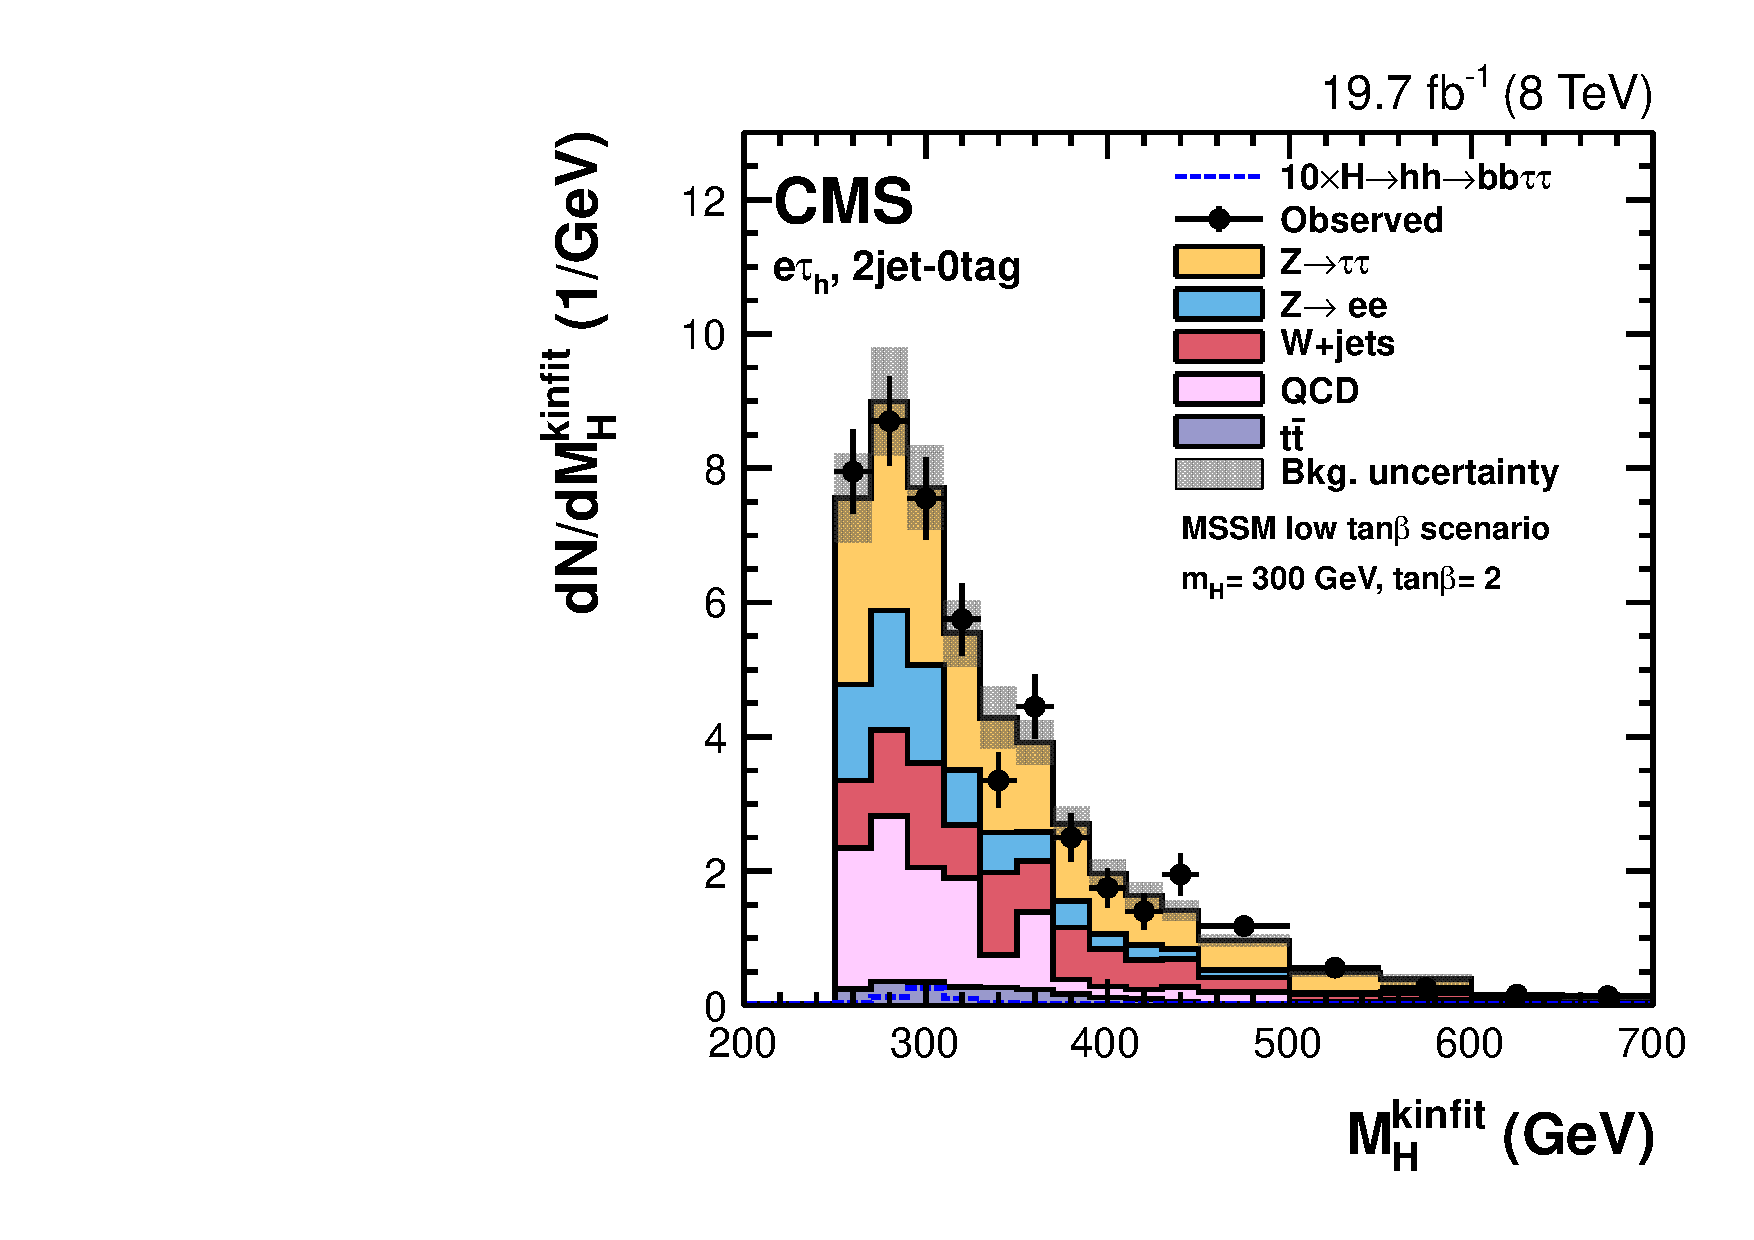
\includegraphics[width=0.5\textwidth]{Hhh/Plots/CMS-HIG-14-034_Figure_004-a.pdf}}
\subfloat[2jet-1tag]{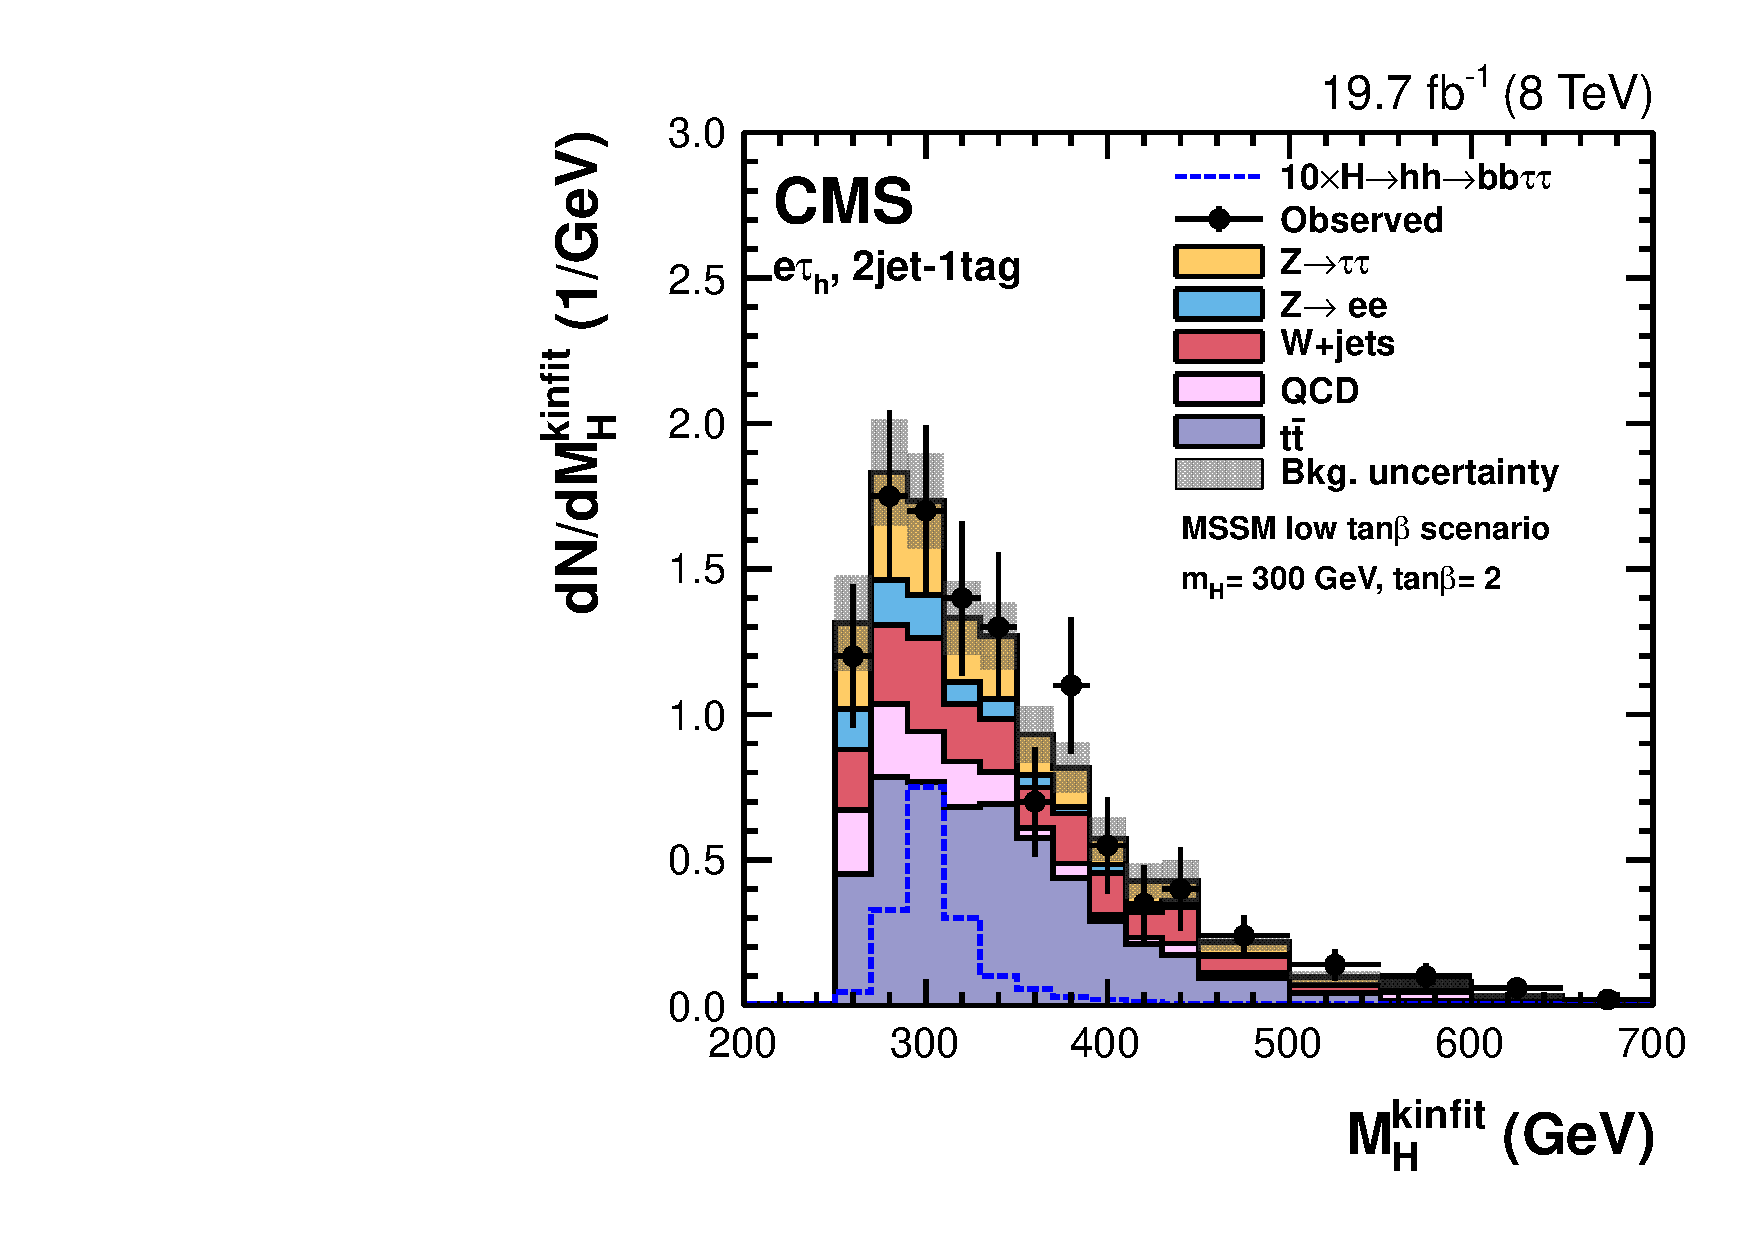
\includegraphics[width=0.5\textwidth]{Hhh/Plots/CMS-HIG-14-034_Figure_004-b.pdf}}~\\
\subfloat[2jet-2tag]{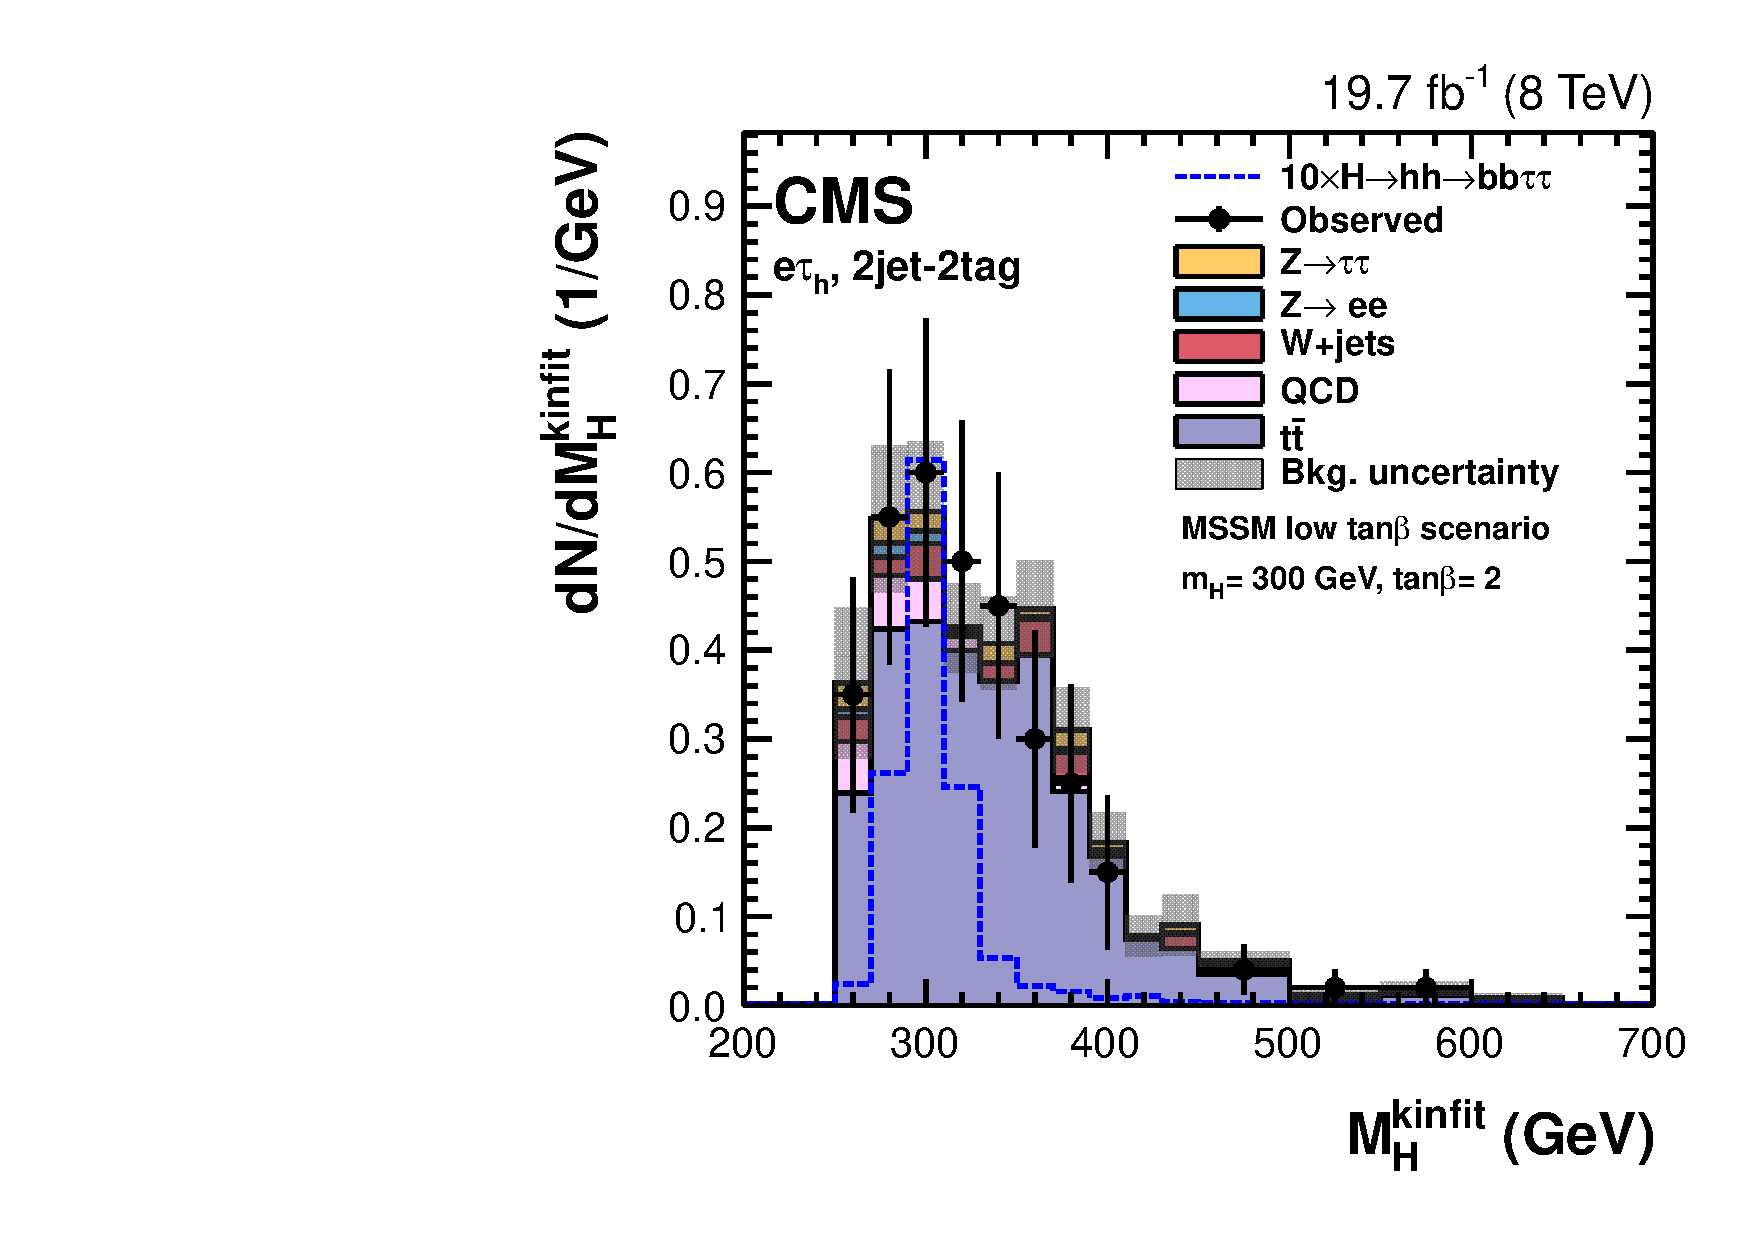
\includegraphics[width=0.5\textwidth]{Hhh/Plots/CMS-HIG-14-034_Figure_004-c.pdf}}
\end{center}
\caption{Distributions of $m_{H}^{kinfit}$ in the 2jet-0tag, 2jet-1tag and 2jet-2tag categories 
of the \etau channel. The \Htohhtobbtautau signal for $m_{H} = 300 $GeV at \tanb=2 in the low\tanb MSSM
scenario, multiplied by 10, is also overlaid. FIXME need to remake these plots!}
\label{fig:hhh_results_mhkinfit_etau}
\end{figure}

None of these distributions show hints of an excess.

The model-independent 95\% CL expected and observed upper limits are shown in 
figure \ref{fig:hhh_results_modelindep}, with figure \ref{fig:hhh_results_modelindep_perchannel}
showing the expected sensitivity per channel. These figures include the contribution from the 
\tautau channel not described in this thesis. Figure \ref{fig:hhh_results_modelindep} shows that
the expected upper limit on the \Htohhtobbtautau process is around 0.3 pb, the observed ranges
from 0.2 pb at low mass to 0.4 pb at high mass. From figure \ref{fig:hhh_results_modelindep}
we can see that the \mutau channel is the most sensitive at masses lower than 320 GeV, with 
the \tautau channel being the most sensitive beyond this mass point. The \etau channel is always
less sensitive than the \mutau channel, but at low mass it is still more sensitive than the \tautau 
channel.

\begin{figure}[h!]
\begin{center}
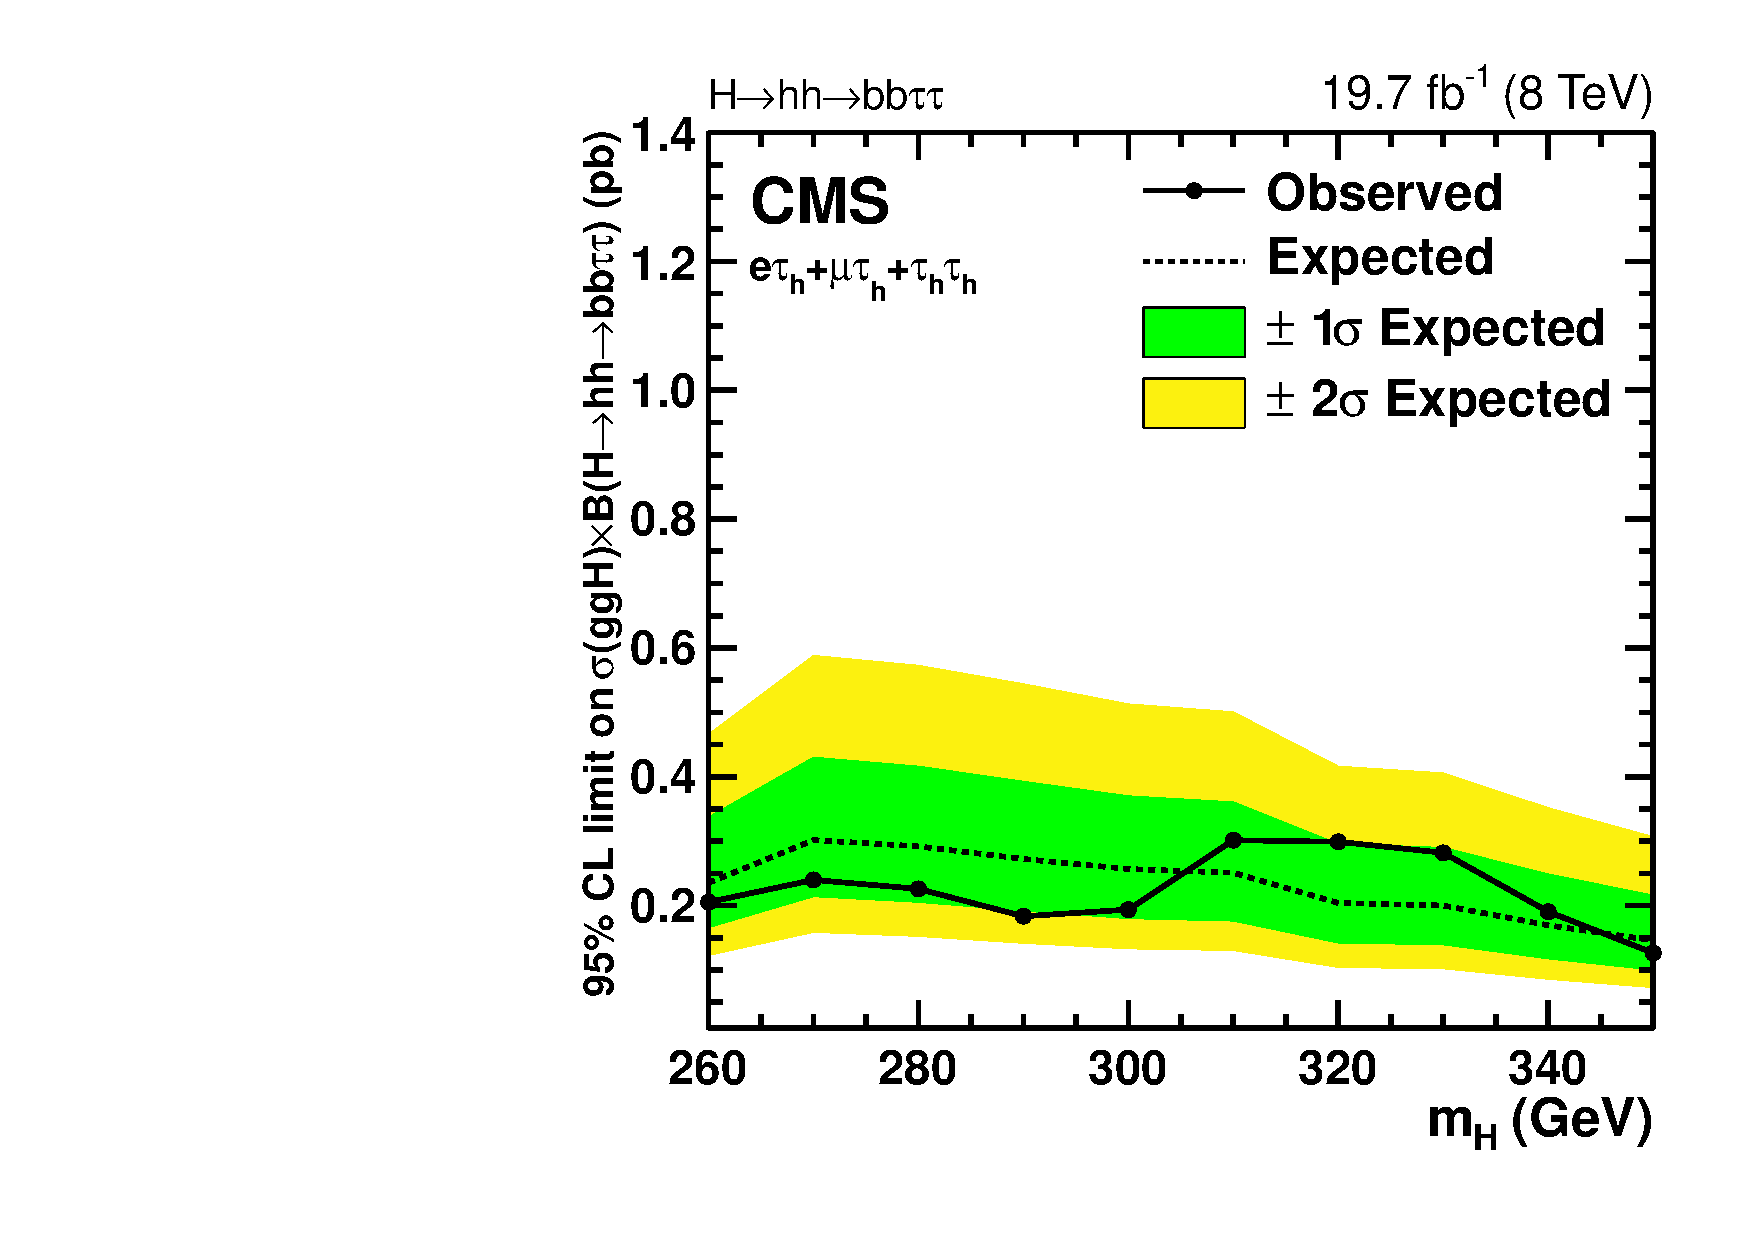
\includegraphics[width=0.7\textwidth]{Hhh/Plots/CMS-HIG-14-034_Figure_008-d.pdf}
\caption{Expected and observed 95\% CL upper limits on cross-section times branching ratio
for the \Htohhtobbtautau process. In these limits the three final states of \etau, \mutau and \tautau are combined \cite{CMS-HIG-14-034}.}
\label{fig:hhh_results_modelindep}
\end{center}
\end{figure}

\begin{figure}[h!]
\begin{center}
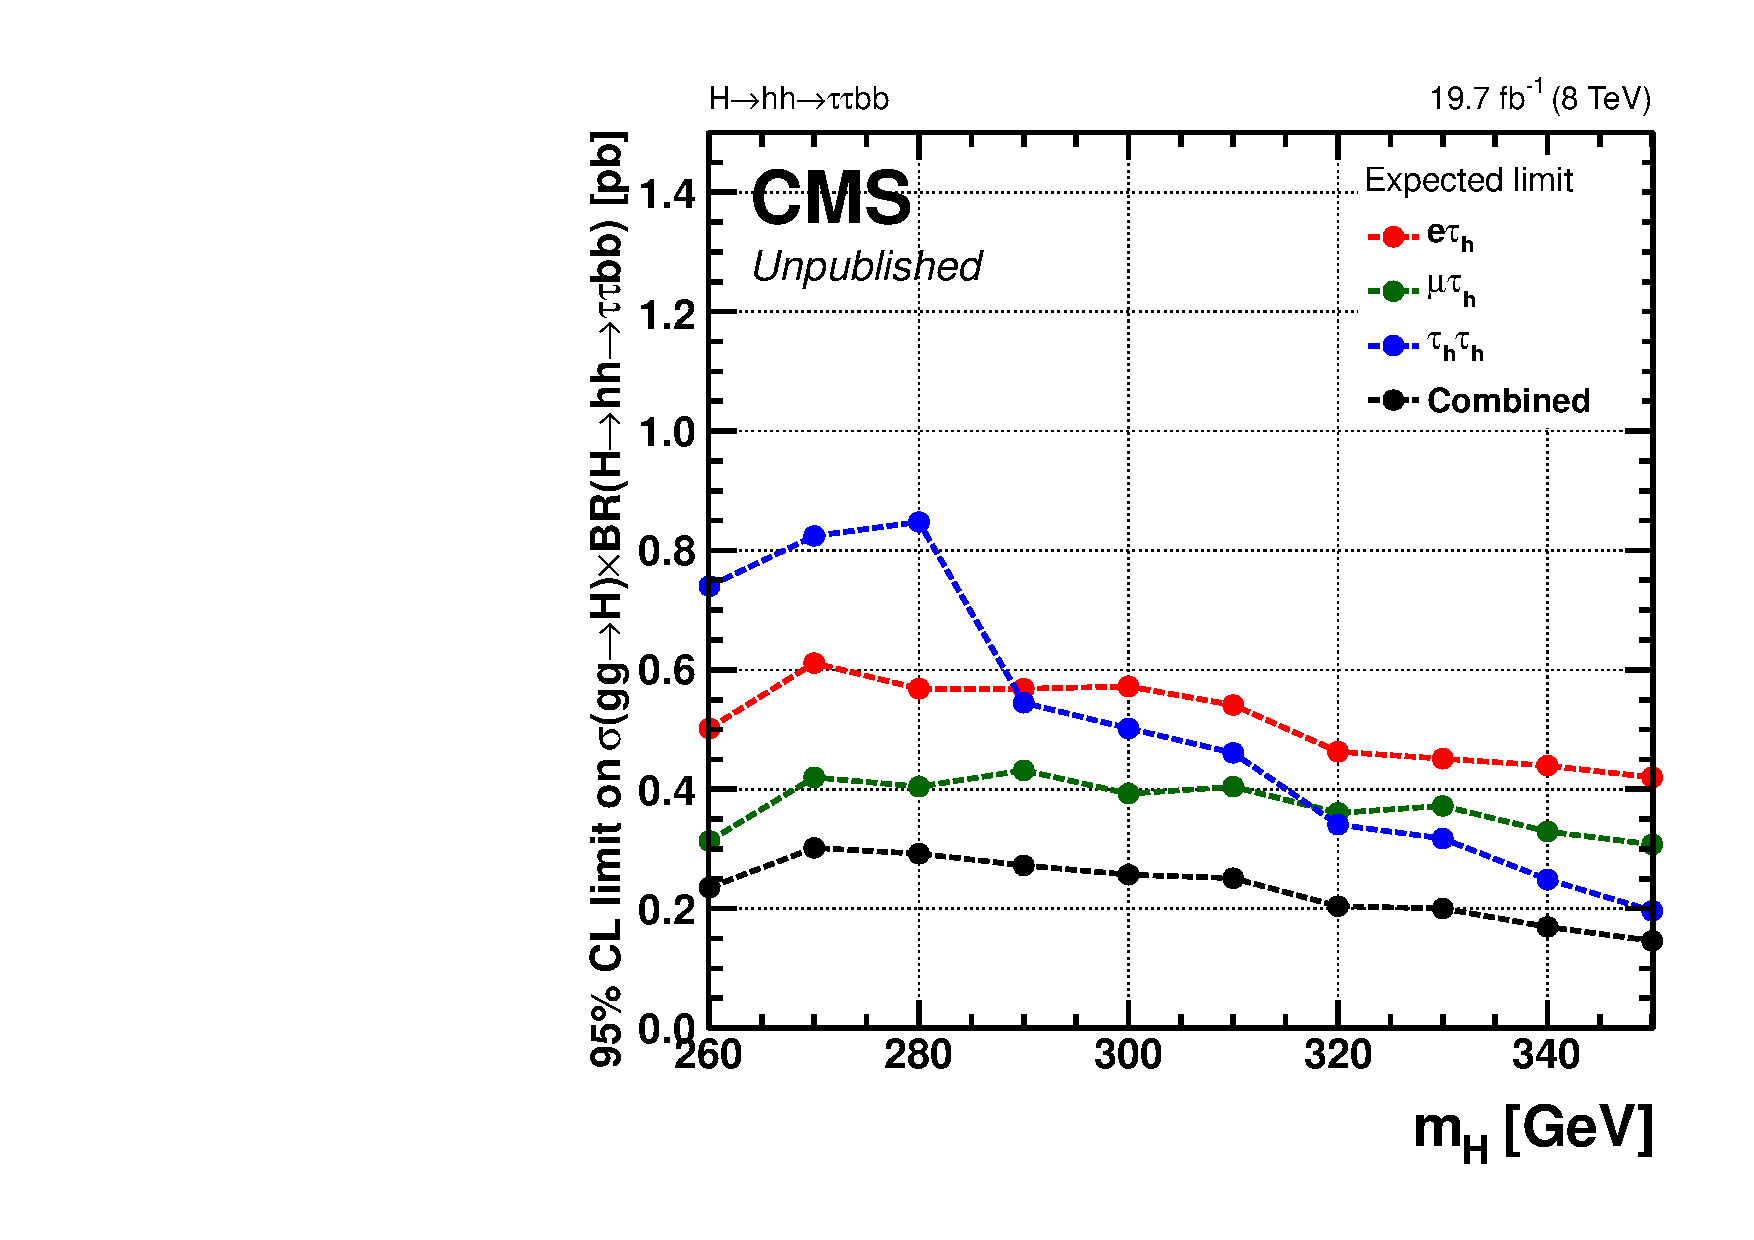
\includegraphics[width=0.7\textwidth]{Hhh/Plots/CMS-HIG-14-034_Figure-aux_033.pdf}
\caption{Expected 95\% CL upper limits on cross-section times branching ratio for the \Htohhtobbtautau process.
The blue line represents the limit for the \tautau channel, the green line for the \mutau channel and the
red line for the \etau channel. The black line shows the limit for all three channels combined. We see that up to around
$m_H = 320$ GeV the \mutau channel is the most sensitive, with the \tautau channel being more sensitive at higher masses. FIXME remake this plot!}
\label{fig:hhh_results_modelindep_perchannel}
\end{center}
\end{figure}


\subsection{Model-dependent results}
\label{sec:hhh_results_modeldep}
The results of the analysis are interpreted in two scenarios, the low \tanb MSSM
scenario, and a type II two--Higgs doublet model (2HDM). 2HDM's are more general
than the MSSM, are not mativated by supersymmetry, and there are several different types. 
Of these different classes, type II 2HDM's are most studied
as the couplings of the MSSM form a subset of the couplings in type II 2HDMs. 

\subsubsection{Interpretation in a type II 2HDM}
\label{sec:hhh_results_modeldep_2HDM}
A 2HDM of type II has more free parameters than a specified MSSM scenario: the physical masses of the Higgs bosons (\mh, \mH,
\mA, \mHplus), the ratio of the vacuum expectation values of the two Higgs doublets (\tanb),
the CP-even Higgs mixing angle ($\alpha$) and $m_{12}^{2} = m_{\PHiggsps}^{2}[\tan{\beta}/(1+\tan{\beta}^2)]$.
To leave two free parameters, it is enough to fix the masses of the physical Higgs bosons. For this
interpretation the assumption that \mA = \mH = \mHplus = $300$~GeV, and \mh = $125$~GeV, is made.

The couplings of the Higgs bosons to quarks and leptons, and of heavy Higgs bosons to other
particles, are defined by $\alpha$ and $\beta$, as in table \ref{tab:hhh_2HDM_couplings}.

\begin{table}[htdp]
\begin{center}
\caption{Couplings in the type II 2HDM}
\begin{tabular}{@{}ll@{}}
%\toprule
\textbf{Decay} & \textbf{Coupling}\\
\midrule
$\PHiggslight \rightarrow$ up--type quarks & $\text{SM coupling} \times \frac{\cos{\alpha}}{\sin{\beta}}$ \\
$\PHiggslight \rightarrow$ down--type quarks, leptons & $\text{SM coupling} \times -\frac{\sin{\alpha}}{\cos{\beta}}$ \\
$\PHiggs \rightarrow \PHiggslight\PHiggslight$ & $\sim$ \cosba $\times$ terms containing masses,\\
 & mixing angles, quartic couplings \\
$\PHiggsps \rightarrow \PZ\PHiggslight$ & $\sim$ \cosba\\
%\bottomrule
\end{tabular}
\label{tab:hhh_2HDM_couplings}
\end{center}
\end{table}

FIXME: ALIGNMENT LIMIT


The interpretations are made in the \cosba--\tanb plane. Figures \ref{fig:Hhh2HDMOverlaid}
and \ref{fig:AZh2HDMOverlaid} show the observed and expected exclusion at 95\% confidence level for the \Htohh
and \AtoZh analyses respectively, overlaid on the production cross--section times branching ratio.
The exclusion contours have some interesting features, most of which can be explained by the couplings
from table \ref{tab:hhh_2HDM_couplings}. When \cosba=0, in the alignment limit, the couplings
of all particles are exactly standard model--like. This is reflected in the \Htohh and \AtoZh branching ratios, 
which both vanish as \cosba approaches 0. This leads to the corridor of non--exclusion down the 
centre of figures \ref{fig:Hhh2HDMOverlaid} and \ref{fig:AZh2HDMOverlaid}. Additionally,
as the couplings of \PHiggslight to pairs of b--quarks and $\Pgt$ leptons are porportional 
to $\frac{\sin{\alpha}}{\cos{\beta}}$, the branching ratios of \Htohhtobbtautau
and \AtoZhtolltautau vanish when $\alpha = 0$, leading to the corridor of non--exclusion
at \cosba $ > 0$ and low \tanb in the \AtoZh figure. A similar corridor is starting
to become visible in the $\sigma \times BR$ structure of the \Htohh interpretation, but
the analysis is not yet sensitive enough to actually see a full--blown corridor in this
region.
Additional regions of non--exclusion at low \tanb and \cosba near -1 are visible in the \Htohh 
interpretation, these are a result of the complex \Htohh branching ratio (ADD FIGURE).




\begin{figure}[h!]
\begin{center}
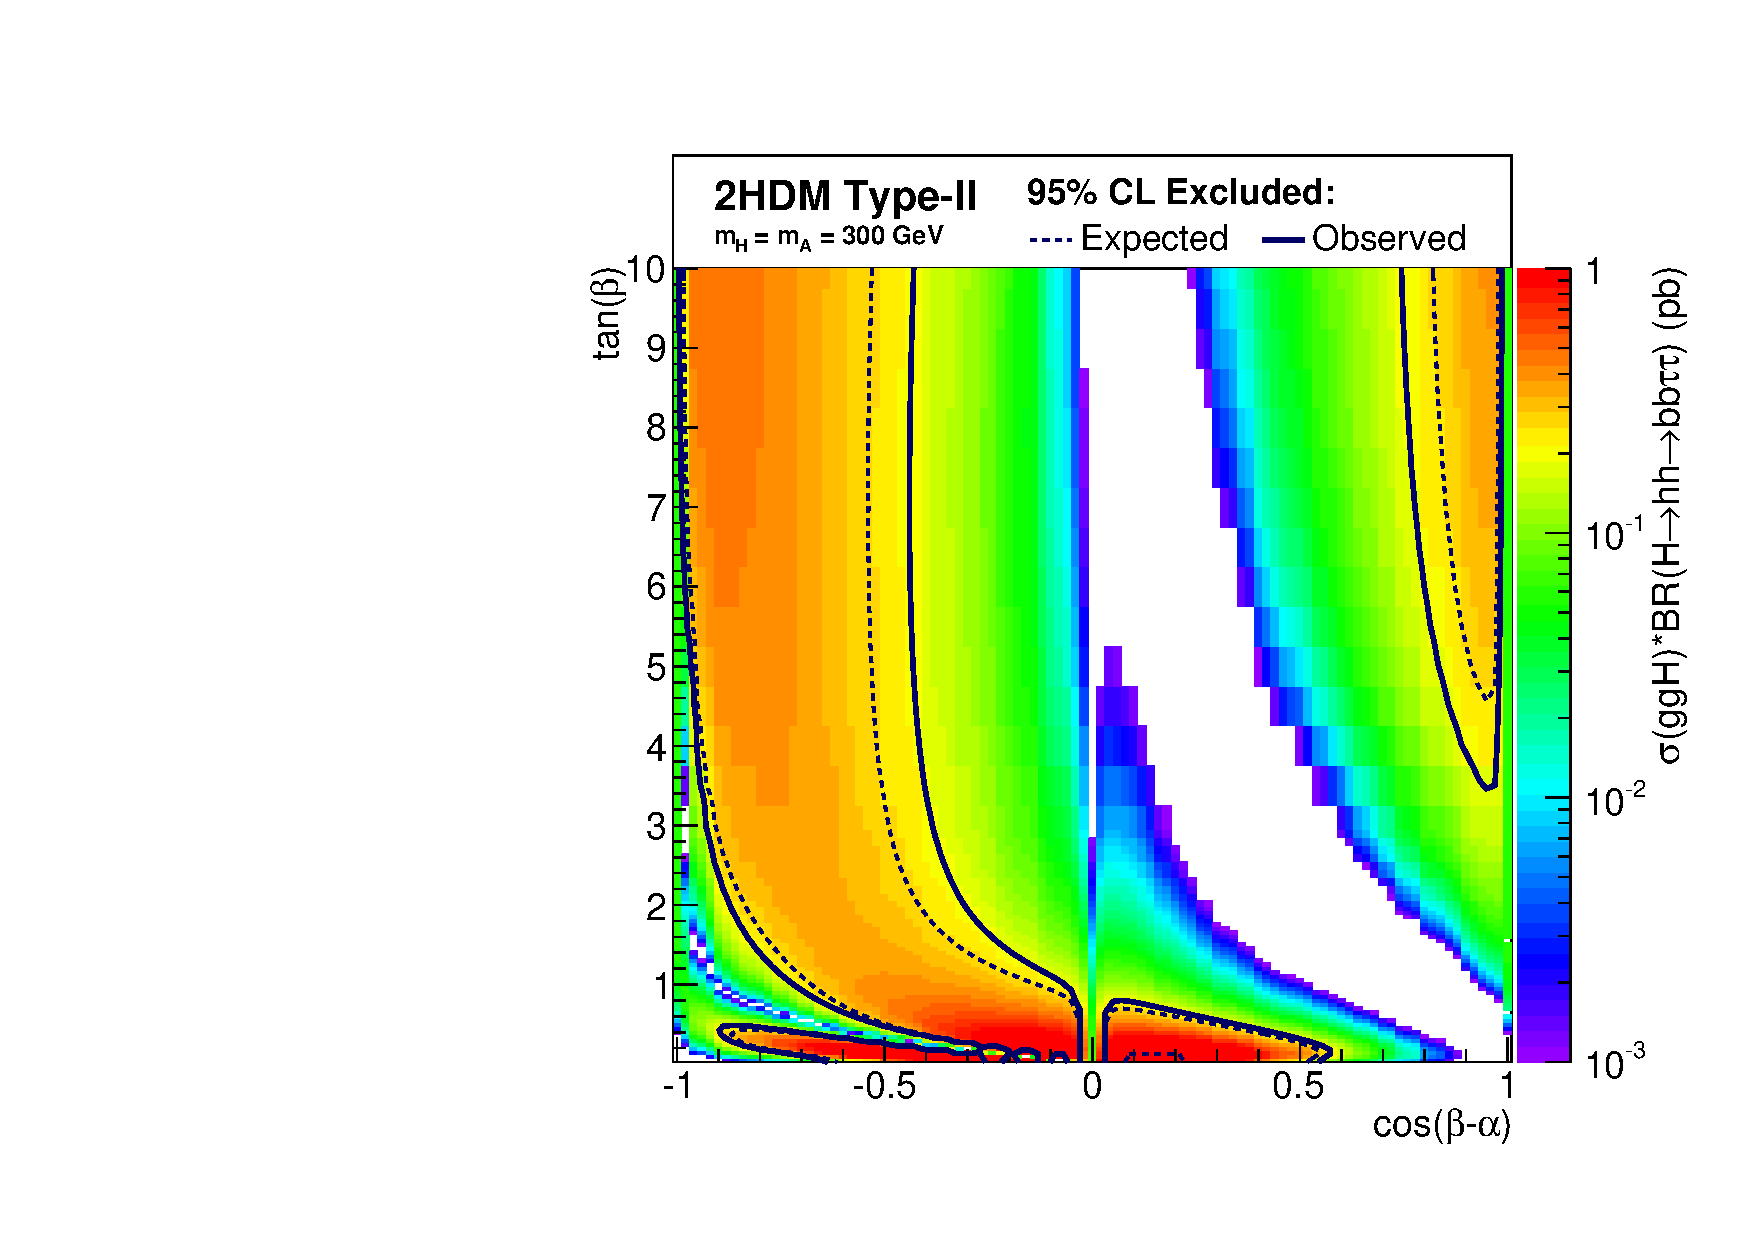
\includegraphics[width=0.85\textwidth]{Hhh/Plots/Hhh2HDM.pdf}
\caption{Search for \Htohhtobbtautau interpreted in a type II 
2HDM, assuming $m_{H} = m_{A} = m_{H^{+}} = 300$ GeV. The expected (dashed line)
and observed (solid line) exclusion contours at 95\% confidence level are overlaid
on the cross--section of $gg\rightarrow \PHiggs$ production
times the branching ratio of \PHiggs into \hhtobbtautau.
Regions of the \cosba-\tanb plane where the cross--section times branching
ratio is larger than the model-independent upper limit set for $m_{H} = 300 $~GeV 
(see figure \ref{fig:hhh_results_modelindep}) are excluded.}
\label{fig:Hhh2HDMOverlaid}
\end{center}
\end{figure}

\begin{figure}[h!]
\begin{center}
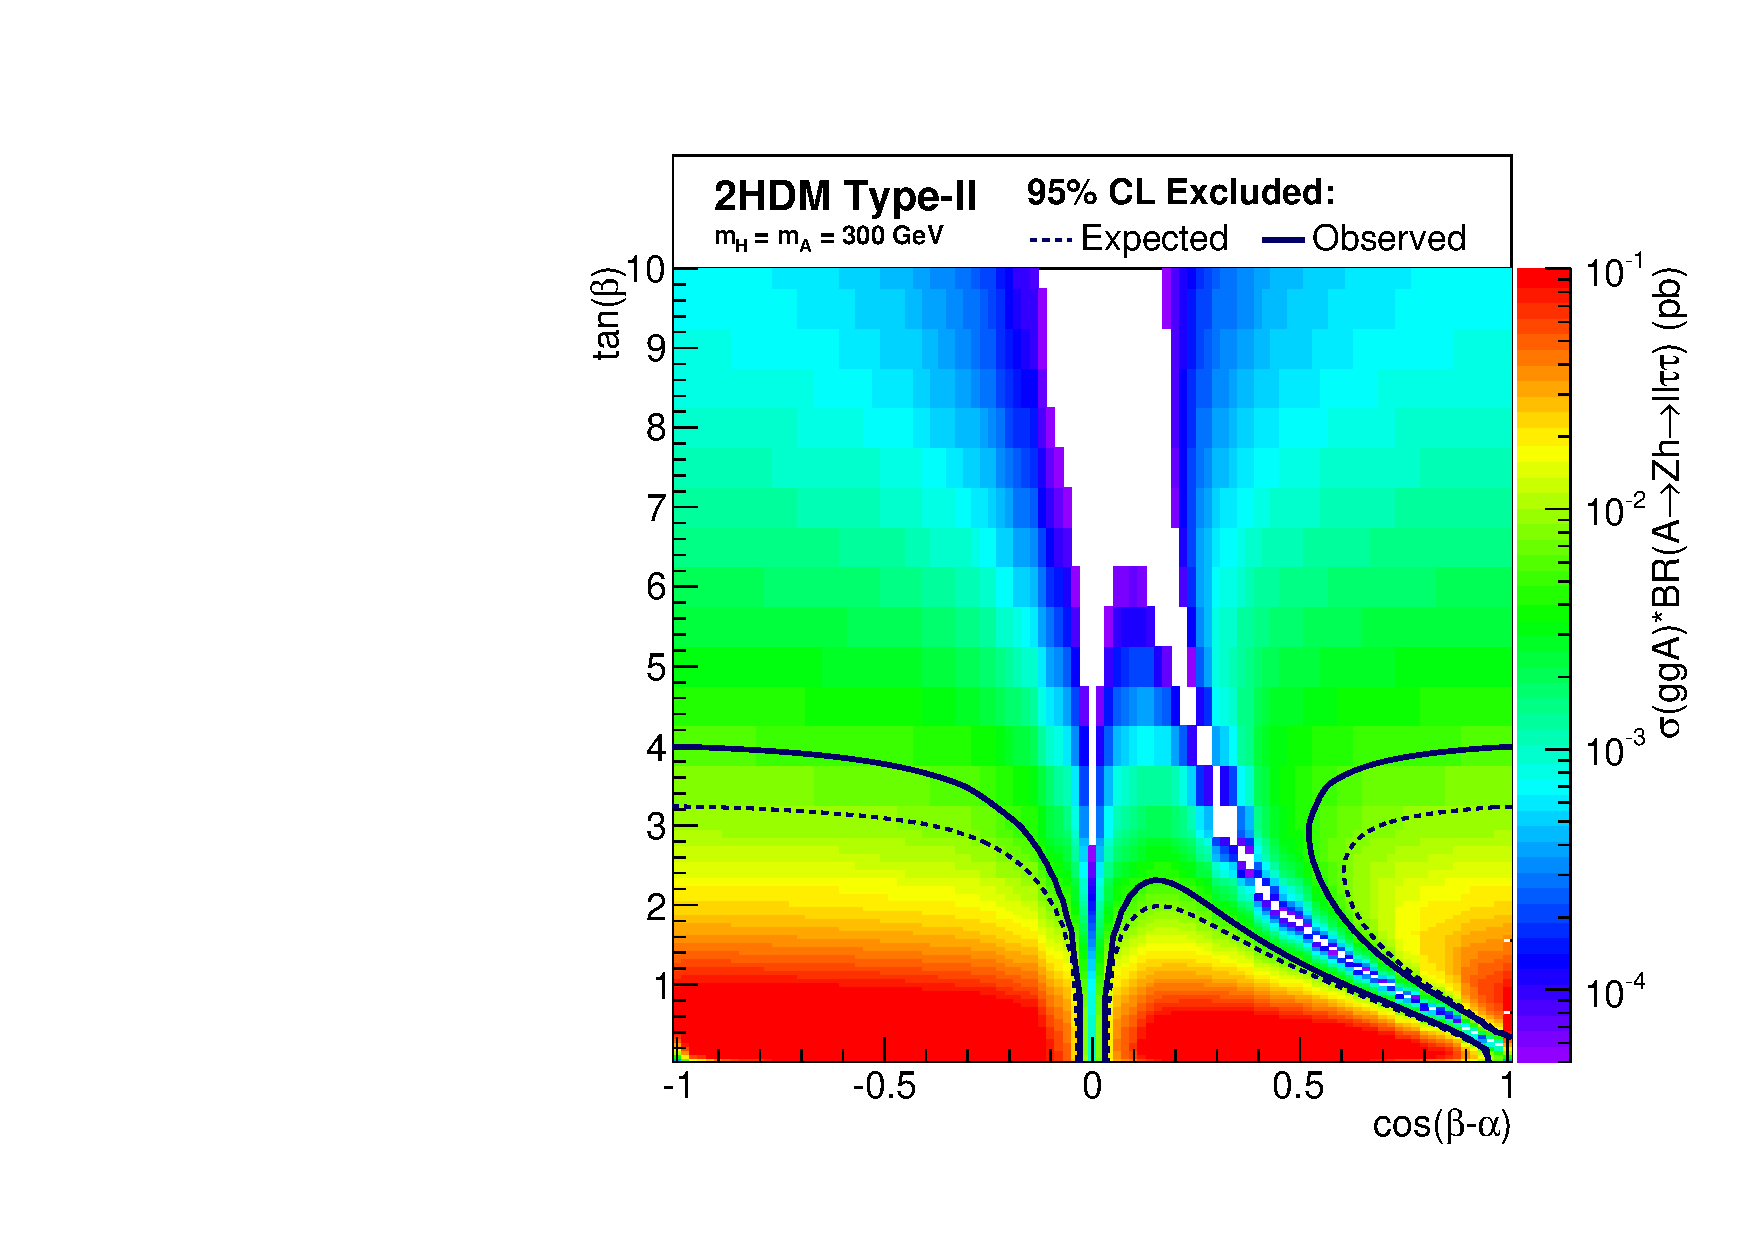
\includegraphics[width=0.85\textwidth]{Hhh/Plots/AZh2HDM.pdf}
\caption{Search for \AtoZhtolltautau interpreted in a type II 
2HDM, assuming $m_{H} = m_{A} = m_{H^{+}} = 300$ GeV. The expected (dashed line)
and observed (solid line) exclusion contours at 95\% confidence level are overlaid
on the cross--section of $gg\rightarrow \PHiggsps$ production
times the branching ratio of \PHiggsps into \Zhtolltautau.
Regions of the \cosba-\tanb plane where the cross--section times branching
ratio is larger than the model-independent upper limit set for $m_{A} = 300 $~GeV 
(see figure \ref{fig:AZhUpperLimits}) are excluded.}
\label{fig:AZh2HDMOverlaid}
\end{center}
\end{figure}

A combined interpretation of both analyses in this model is presented
in figure \ref{fig:HhhAZh2HDM}. Some of the features discussed earlier
in this section are also visible in this combined interpretation.

\begin{figure}[h!]
\begin{center}
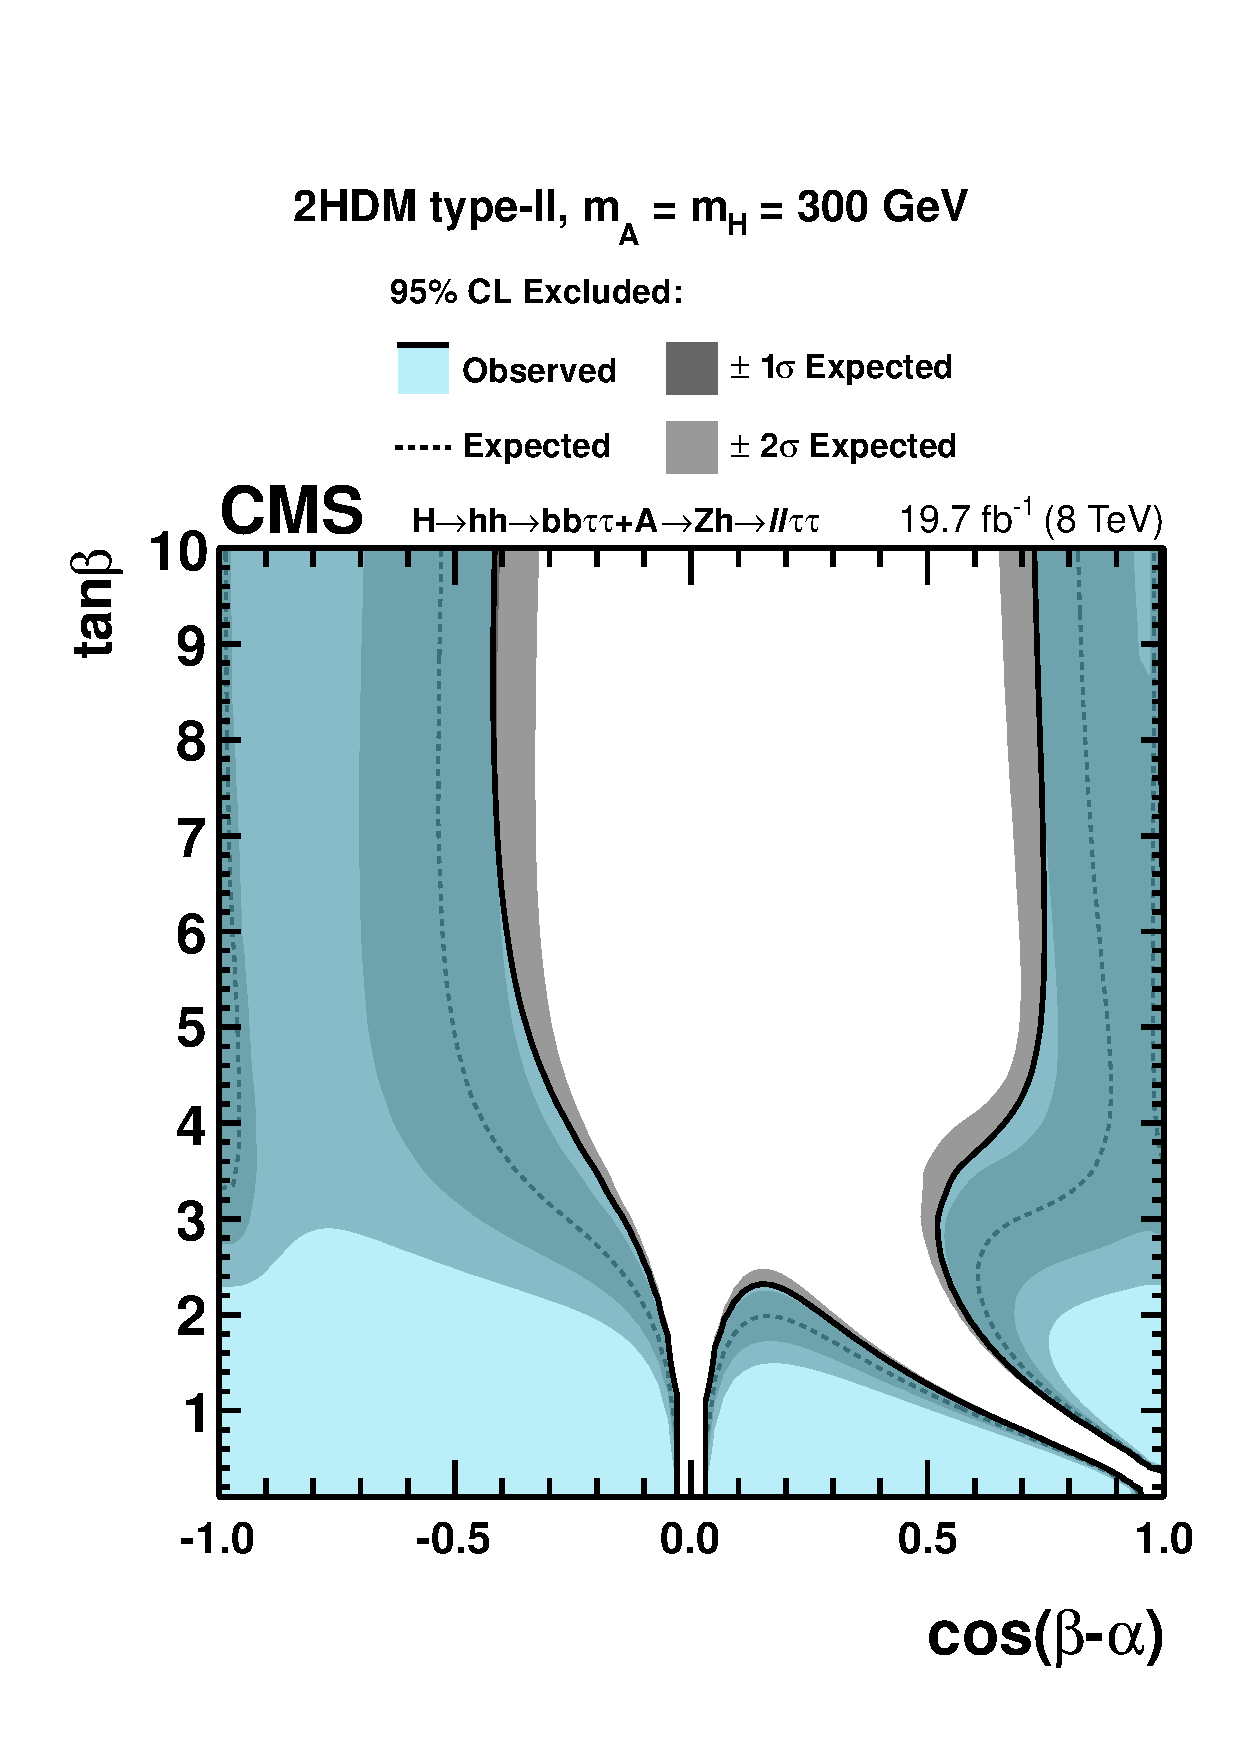
\includegraphics[width=0.85\textwidth]{Hhh/Plots/CMS-HIG-14-034_Figure_012.pdf}
\caption{Combined interpretation of searches for \AtoZhtolltautau and 
\Htohhtobbtautau in a type II 2HDM, assuming $m_{H} = m_{A} = m_{H^{+}} = 300$ GeV.
The shaded blue area bounded by the solid black line indicates the observed 
95\% confidence level excluded region. The dashed black line indicates the expected
exclusion, with the grey bands indicating the $\pm 1\sigma$ and $2\sigma$ 
exclusion limits \cite{CMS-HIG-14-034}.}
\label{fig:HhhAZh2HDM}
\end{center}
\end{figure}

\subsubsection{Interpretation in the low \tanb MSSM scenario}
\label{sec:hhh_results_modeldep_lowtb}
The low \tanb MSSM scenario, as discussed in section FIXME: write theory section that mentions this
is an MSSM scenario that has been adapted to allow \mh $=125 \pm 3$~GeV for \tanb values
as low as 1.  

Figure \ref{fig:Hhhlowtanb} shows the cross-section times branching ratio
of the \Htohhtobbtautau process in the MSSM low \tanb scenario. Comparing these values 
to the expected and observed upper limits in figure \ref{fig:hhh_results_modelindep} one
can see that the cross-section times branching ratio in this model is, with exception of a few small 
areas, lower than the upper limits set by this analysis. This analysis on its own is
therefore not sensitive enough to exclude any of the \mA-\tanb region in this model. Note that
at low \tanb ~ \mA and \mH are degenerate, and therefore \mH is not in the studied range of $260-350$ GeV
throughout the entire \mA-\tanb plane shown here.

\begin{figure}[h!]
\begin{center}
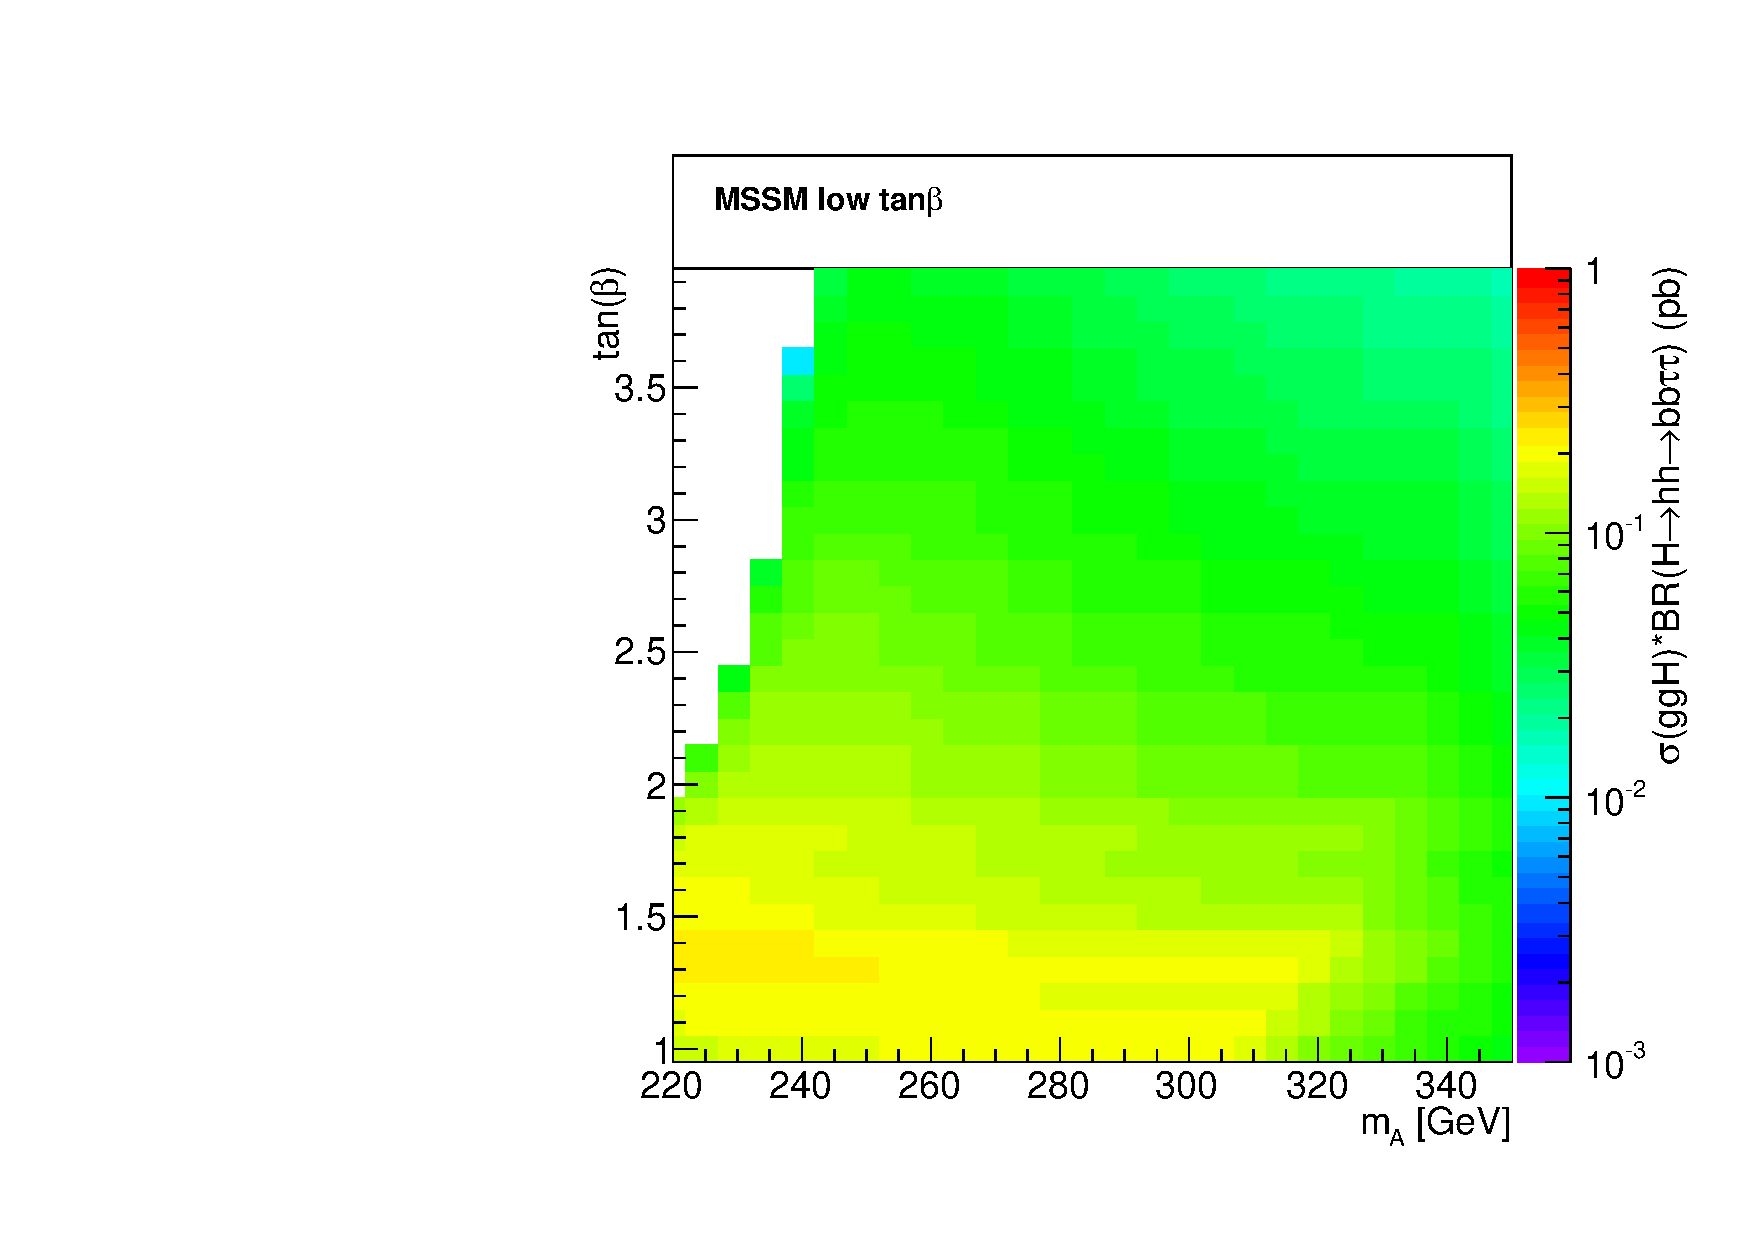
\includegraphics[width=0.85\textwidth]{Hhh/Plots/Hhhlowtbhigh.pdf}
\caption{Cross-section times branching ratio of the \Htohhtobbtautau process
in the low-\tanb MSSM scenario. No expected and observed exclusion contours
have been overlaid on these figures as the cross-section times branching
ratio is smaller than the upper limits set in figure \ref{fig:hhh_results_modelindep}.}
\label{fig:Hhhlowtanb}
\end{center}
\end{figure}

The \AtoZhtolltautau analysis on the other hand can exclude parts of the \mA-\tanb region
in this model by itself. The expected and observed 95\% CL exclusion contours are overlaid 
on the cross-section times branching ratio for this process in the low \tanb MSSM scenario in
figure \ref{fig:AZhlowtanbOverlaid}. The sharp drop in cross-section times branching ratio, and therefore exclusion,
near \mA $ = 350$ GeV arises from the fact that near this mass the decay $\PHiggsps \rightarrow t\bar{t}$ becomes
kinematically allowed, resulting in a reduction of the \AtoZh branching ratio.


\begin{figure}[h!]
\begin{center}
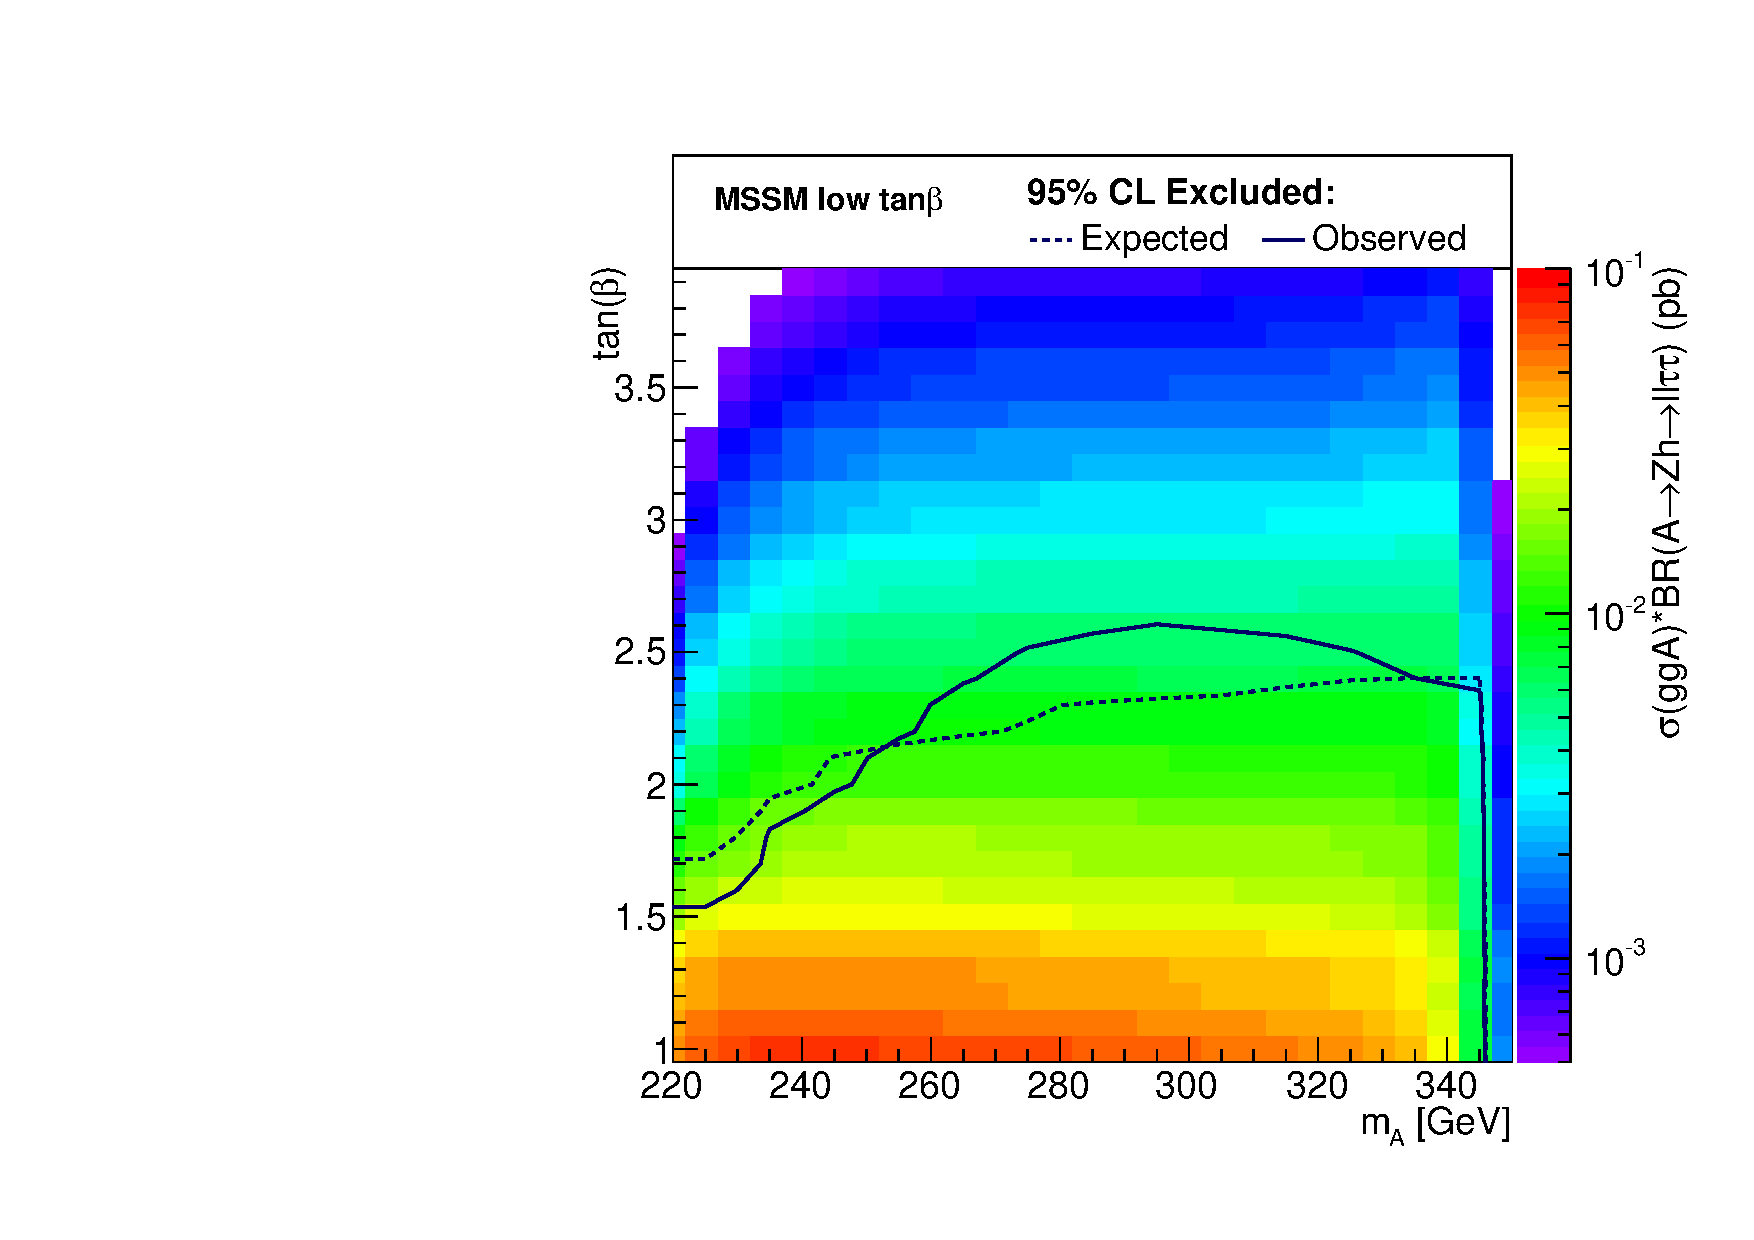
\includegraphics[width=0.85\textwidth]{Hhh/Plots/AZhlowtbhigh.pdf}
\caption{Expected and observed 95 \% CL exclusion limits for the \AtoZhtolltautau analysis
in the low \tanb MSSM scenario, overlaid on the cross-section times branching ratio. Areas where
the cross-section times branching ratio is larger than the upper limits in figure \ref{fig:AZhUpperLimits}
are excluded. The exclusion rapidly drops off at $m_A = 350$ GeV due to the turn-on of the
$ \PHiggsps \rightarrow$ \ttbar process.}
\label{fig:AZhlowtanbOverlaid}
\end{center}
\end{figure}


The combined interpretation of both analyses in this model is presented in figure \ref{fig:HhhAZhMSSM}.
The exclusion in this scenario is driven by the \AtoZh search as the \Htohh search is not
very sensitive in this model. Combining the two analyses we do see that a slightly larger amount
of the \mA-\tanb plane can be excluded than using the \AtoZhtolltautau analysis alone. The features
described for figure \ref{fig:AZhlowtanbOverlaid} are also visible in this figure. A small region of phase
space, at low \mA and low\tanb predicts a light Higgs boson mass that is not compatible with 125 GeV within 3 GeV.
This region is therefore excluded, this is indicated by the red band. 

\begin{figure}[h!]
\begin{center}
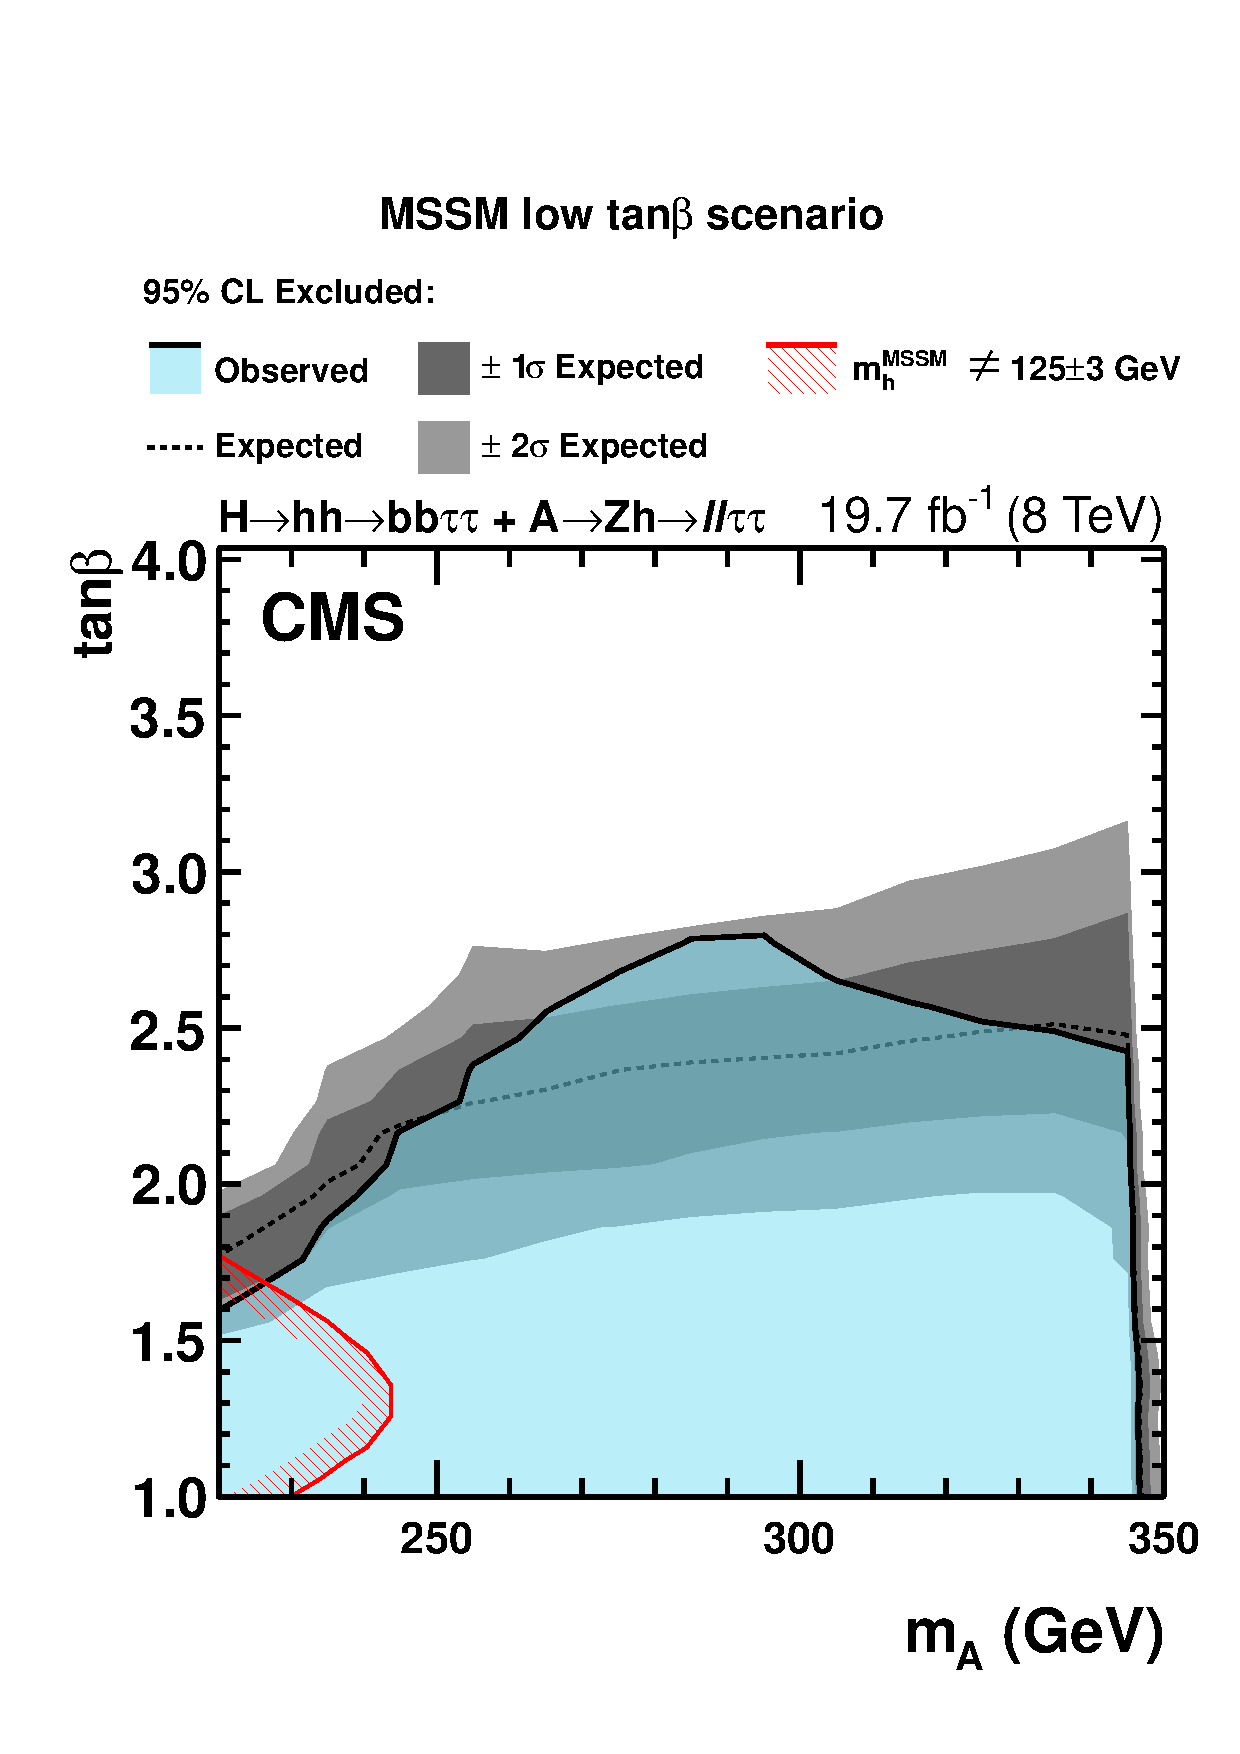
\includegraphics[width=0.85\textwidth]{Hhh/Plots/CMS-HIG-14-034_Figure_011.pdf}
\caption{Combination of the \AtoZhtolltautau and \Htohhtobbtautau searches
interpreted in the low \tanb MSSM scenario. The shaded blue area bounded by
the solid black line indicates the observed excluded region at 95\% confidence level.
The dashed black line indicates the expected exclusion, with the grey bands showing
the $\pm 1\sigma$ and $2\sigma$ expected exclusion \cite{CMS-HIG-14-034}. The area
bounded by the red line is the region of phase space where \mh $\neq 125 \pm 3$ 
GeV and is therefore not accessible.}
\label{fig:HhhAZhMSSM}
\end{center}
\end{figure}
